\documentclass[10pt, a4paper, oneside, titlepage]{book}

\usepackage[utf8]{inputenc}
\usepackage[T1]{fontenc}
\usepackage{lmodern, textcomp}
\usepackage[english, french]{babel}
\usepackage{csquotes}

\usepackage[activate={true,nocompatibility}, final, babel=true
	tracking=true, kerning=true, spacing=true,
	factor=1100, stretch=10, shrink=10]{microtype}

\usepackage[top=4cm, bottom=3.5cm, left=3.5cm, right=3.5cm]{geometry}
% default top=4.5cm, bottom=4cm, left=4.5cm, right=4.5cm
\usepackage{changepage}

\usepackage{eurosym, xspace}
\usepackage[nottoc]{tocbibind}
\usepackage{graphicx, subfig, float}
\usepackage[multiple]{footmisc}
\usepackage{authblk}
\usepackage[backend=bibtex8, citestyle=numeric-comp, maxbibnames=99, sorting=nyt,
			sortcites=true, firstinits=true]{biblatex}
% TODO: améliorer le style
/home/harold/texmf/tex/latex/biblatex/escrime.def

\usepackage{amsmath, amsfonts, amssymb, siunitx}

\usepackage{makeidx}
\usepackage[cc]{titlepic}

\usepackage[usenames, dvipsnames]{xcolor}
\usepackage{framed, mdframed}
\usepackage[amsmath, hyperref, framed]{ntheorem}
% \usepackage{amsthm, thmtools}


% hyperfootnotes=false
\usepackage[pdftex, colorlinks=true, breaklinks=true,
	urlcolor=blue, linkcolor=blue, citecolor=red,
	pdfcreator={PDFLaTeX}, pdfauthor={Harold Erbin}
]{hyperref}
\usepackage[all]{hypcap}

\usepackage[sort&compress, nameinlink, french]{cleveref}


\usepackage{escrime}


\hypersetup{
	pdftitle={Arts martiaux historiques - manuel},
	% pdfkeywords={Mots clés PDF},
	% pdfsubject={Sujet PDF}
}


\renewcommand{\Affilfont}{\small}
\newcommand{\email}[1]{\thanks{\href{mailto:#1}{\nolinkurl{#1}}}}
% \sisetup{group-separator = {,}, separate-uncertainty=true}
% enable non-breakable space
\DeclareUnicodeCharacter{00A0}{~}
\DeclareUnicodeCharacter{202F}{~}


% \SetExtraKerning[unit=space]{
% 		encoding={*}, family={bch}, series={*},
% 		size={footnotesize, small, normalsize}
% 	}{
% 		\textendash={400,400}
% }
\SetTracking{encoding={*}, shape=sc}{0}
% \microtypecontext{spacing=french}


\pagestyle{plain}
\graphicspath{{images/}}


\addbibresource{escrime}
\iffalse
\bibliography{escrime}
\fi

\makeindex


\title{Arts martiaux historiques -- manuel}

\author[*]{Harold Erbin\email{harold.erbin@gmail.com}}
\affil[*]{Chapitre des armes, Paris, France}
\affil[*]{Club d'escrime ancienne, École Normale Supérieure, Paris, France}

\titlepic{
\includegraphics[width=0.8\textwidth]{logo_cda.pdf}}


\begin{document}

% \pagenumbering{roman}
\maketitle


% \pagenumbering{arabic}
\setcounter{page}{2}

\thispagestyle{empty}
\begin{center}
	\setlength{\baselineskip}{1.5\baselineskip}{\fontsize{12}{14}\selectfont{}
	Ce texte est diffusé sous la licence libre\\\textbf{Licence Art Libre} :}\\\url{http://artlibre.org/licence/lal/}
\end{center}

\vspace{\stretch{2}}

\noindent
% {\setlength{\tabcolsep}{0.5ex}
\begin{tabular}{ll}
	Sites du projet : &
		\url{https://github.com/melsophos/manuel-amhe} \\
		&
		\url{https://chapitredesarmes.wordpress.com/travaux} \\
	Téléchargement : & 
		\url{https://www.dropbox.com/s/ga9t604bu94rmox/amhe_manuel.pdf}
\end{tabular}
% }

% \vspace{\stretch{1}}


\clearpage
\pdfbookmark[1]{\contentsname}{toc}
\microtypesetup{protrusion=false}
\tableofcontents
\microtypesetup{protrusion=true}


\chapter{Introduction}


%%%%%%%%%%%%%%%%%%
\section{Objectif}
%%%%%%%%%%%%%%%%%%


\index{\textsc{Amhe}}
\index{arts martiaux traditionnels}

Ce manuel est une compilation d'outils, de techniques et d'exercices pour pratiquer les \emph{arts martiaux historiques}, principalement \emph{européens} (\textsc{Amhe}) et incluant l'escrime médiévale~\footnotemark{}.
\footnotetext{Un terme plus adapté pourrait être simplement \emph{arts martiaux traditionnels}.
En effet il est fréquent de chercher l'inspiration dans d'autres styles, modernes ou asiatiques, lorsque les sources font défaut ; de plus l'étude d'autres arts martiaux pourrait trouver sa place dans cette approche (comme les arts du combat en Amérique pré-colombienne).}
Le but n'est pas de fournir une étude détaillée d'une arme ou d'un style particulier mais plutôt d'offrir un panel dans lequel on pourra piocher pour découvrir ses goûts et acquérir une culture générale.
Diverses annexes complètent le texte, par exemple sur les principaux traités et sur la fabrication de matériel.
En particulier les convention adoptées sont décrites dans l'annexe~\ref{app:conventions}.


%%%%%%%%%%%%%%%%%%%
\section{Ce manuel}
%%%%%%%%%%%%%%%%%%%


L'interprétation et l'enseignement des \textsc{Amhe} comportent une certaine part de sensibilité personnelle.
En particulier ce manuel reflète notre manière d'aborder l'escrime et a été influencée par les échanges au cours de notre pratique, mais rien ne garantit que notre interprétation soit juste ni que notre approche convienne à tous.
Le lecteur est encouragé de réfléchir et d'étudier les sources par lui-même avant de se convaincre que la description est correcte.
Finalement nous rappelons aussi que l'interprétation évolue au cours du temps~\footnotemark{}.
\footnotetext{Cela peut se voir en comparant les vidéos sur Youtube au sujet d'un même manuscrit à une dizaine d'années d'intervalle.}
% Finalement il est toujours utile d'étudier des interprétations qui diffèrent des nôtres et de les garder sous la main afin de fournir une base de travail.
Une grande partie du matériel présenté est issu des cours donnés par le Chapitre des armes et le club d'escrime ancienne de l'\textsc{Ens}.

Ce manuel est un \textbf{brouillon} et la qualité des différents chapitres est inégale, toutefois nous pensons que ce texte peut déjà servir en l'état actuel.
À terme l'objectif est de compléter chaque chapitre avec une introduction générale, des références aux sources, des exercices et des techniques, des schémas et des figures ainsi qu'une analyse du style.
Les remarques, critiques et suggestions sont extrêmement bienvenues et peuvent être soumises sur Github~\footnotemark{} (méthode privilégiée) ou envoyées par mail.
\footnotetext{\url{https://github.com/melsophos/manuel_amhe/issues}}

L'intégralité des sources Latex peut être téléchargées sur Github~\footnotemark{}.
\footnotetext{\url{https://github.com/melsophos/manuel_amhe}}
De cette manière n'importe quelle partie du texte peut être réutilisée, par exemple pour un document plus spécialisé ou pour préparer un atelier (à condition de respecter la licence Art libre).
Les modifications entre deux versions peuvent être trouvées dans le fichier \texttt{CHANGES} qui se trouve sur Github.


%%%%%%%%%%%%%%%%%%%%%%%%%%%%%%%%%%%%%
% \section{Arts martiaux traditionnels}
%%%%%%%%%%%%%%%%%%%%%%%%%%%%%%%%%%%%%



%%%%%%%%%%%%%%%%%%
\section{Pratique}
%%%%%%%%%%%%%%%%%%


\noindent
La pratique des \textsc{Amhe} contient plusieurs aspects ainsi que des activités connexes :
\begin{itemize}
	\item la pratique en groupe (sous la tutelle d'un instructeur) ;
	\item l'étude des sources et l'essai en groupe réduit ;
	\item le combat libre (mise en pratique en situation "réelle") ;
	\item les compétitions sportives (tournois) ;
	\item les démonstrations et spectacles (par exemple en fête médiévale).
\end{itemize}
Finalement les entraînements comprennent souvent une part de musculation afin d'être en meilleure forme physique et d'éviter les blessures (à court ou long terme).
Il n'est pas forcément nécessaire d'étudier soi-même les sources pour faire des progrès pendant un certain temps.
De même, bien que le combat libre est très utile afin de progresser, rien n'oblige à en faire, et encore moins à participer à des tournois.
Finalement il peut être intéressant d'étudier l'escrime de spectacle afin de faire de belles démonstrations et de mieux partager notre intérêt, mais encore une fois ce n'est pas une obligation.
Ainsi il n'y a pas de programme fixée une fois pour toute et chacun peut adapter son étude par rapport à ses centres d'intérêts.


% TODO: déplacer dans un chapitre à part, avec la mentalité générale (objectif d'entraînement, etc.)
Avant de continuer nous souhaitons aborder un point important qui peut avoir un impact négatif sur les progrès que l'on peut faire.
Il est fréquent de rencontrer des étudiants qui vont dire que telle technique étudiée ne marche pas car il existe un contre efficace, éventuellement en accélérant beaucoup le geste.
Ceci n'est pas un bon état esprit pour aborder l'escrime car les exercices et les techniques proposés permettent de travailler un élément précis : ils sont créés de telles sortes à ce que l'accent soit mis sur un ou plusieurs points, avec pour objectif d'améliorer la compréhension de l'arme étudiée.
Il existe certainement des contres plus judicieux (surtout si l'on sait ce que l'autre est censé faire en avance ou que l'on va délibérément plus vite que lui) ou d'autres manières de procéder, mais alors on perd l'intérêt de faire cet exercice et le partenaire ne peut plus travailler dans de bonnes conditions.
Cela ne veut pas dire qu'il ne faut pas résister – au contraire il est intéressant de varier le degré de résistance pour progresser –, mais il ne faut pas changer totalement les lignes de la technique (sauf avec accord du partenaire quand l'on souhaite explorer d'autres possibilités).


%%%%%%%%%%%%%%%%%
\section{Sources}
%%%%%%%%%%%%%%%%%


Ce manuel a commencé à croître à partir des cours donnés au club d'escrime ancienne de l'\textsc{Ens} (Paris) par Romain, Thomas et Samuel.
À cette base se sont ajoutés des idées provenant de mes recherches personnelles, de discussion, de stages et de lectures (blog, livres…).
Pour cette raison il est très difficile d'attribuer précisément l'origine de chaque idée et de donner des références exhaustives, en particulier à tous les articles de blog.
Malgré tout je me suis efforcé d'apporter des références précises aux divers auteurs dont je me suis inspiré, en particulier dans les cas suivants : description d'un exercice spécial ou d'un atelier, étude (technique, historique…) détaillée.
De plus la source historique est indiquée pour toute technique où j'ai pu l'identifier.

\index{Wiktenauer}
Le wiki Wiktenauer~\cite{wiktenauer} représente une importante source d'informations : on peut y trouver une biographie des grands maîtres, la transcription (et souvent la traduction) accompagnée des éventuelles illustrations d'un grand nombre de manuscrit ainsi que des liens vers les travaux correspondants (interprétations, livres et traductions dans d'autres langues).
Il s'agit de la première ressource à consulter lorsque l'on cherche une information.

Comme tout domaine spécialisé, les \textsc{Amhe} ont développé un vocabulaire technique assez important, formé en partie des termes employés dans les manuscrits dans la langue d'origine et de leurs traductions.
Pour cette raison de nombreux documents incluent un glossaire.
L'un des glossaires les plus complets pour l'escrime allemande a été compilé par Forgeng~\cite{Forgeng:2002:WalpurgisFechtbuchRoyal}.
La Fédération internationale d'escrime a établi un glossaire pour l'escrime moderne~\cite{FIE:2014:BrefsGlossairesLescrime}.

Finalement un certain nombre de blogs sur les \textsc{Amhe} existent et contiennent des billets sur des sujets variés (pédagogie, interprétation des sources, contexte historique, etc.).
Parmi les plus actifs et intéressants se trouvent : Hroarr~\cite{Blog:Hroarr} (Norling et al.), l'OGN~\cite{Blog:OGN}, Devon Boorman~\cite{Blog:Boorman}, Hans Talhoffer~\cite{Blog:HansTalhoffer} (Kleinau).


%%%%%%%%%%%%%%
\section{Plan}
%%%%%%%%%%%%%%


Tout d'abord le livre n'est pas organisé de manière tout à fait linéaire : les chapitres (surtout au début) sont censés être progressifs, mais parfois nous utilisons des éléments introduits dans des chapitres ultérieurs.
Cela est d'autant plus vrai pour certains exercices qui peuvent utiliser des concepts vus plus tard. 
% Par exemple le chapitre sur les déplacements précède celui sur les attaques et les défenses, mais certains exercices requièrent l'utilisation d'attaques.
Le lecteur est donc encouragé à mettre de côté les parties en question et à y revenir plus tard, ou bien à utiliser l'index pour trouver les informations nécessaires.

La partie~\ref{part:notions-générales} décrit les notions générales telles que la structure du corps, les déplacements, l'attaque et la défense.
Nous conseillons de commencer la lecture par ce chapitre, surtout pour les débutants, et de pratiquer régulièrement les exercices qui y sont donnés.
Ces chapitres requièrent l'utilisation d'une arme mais il n'est pas nécessaire d'avoir étudier les autres parties pour cela car les exercices sont généraux et adaptables à la plupart des armes.

Les parties suivantes sont consacrées à l'étude des armes, qui sont regroupées par grandes familles.
Ces parties et leurs chapitres sont globalement indépendants les uns des autres.

La partie~\ref{part:applications} contient différentes applications et compléments.
Ces chapitres sont relativement indépendants des autres parties.

Finalement différentes annexes apportent des informations supplémentaires sur des sujets connexes.
En particulier les conventions sont décrites dans l'annexe~\ref{app:conventions}.
Un index à la fin du manuel permet de retrouver rapidement une notion recherchée.
Une liste des définitions, des coups et des gardes est donnée dans l'annexe~\ref{app:listes}.

% Nous conseillons au lecteur débutant de jeter un œil aux introductions de chaque chapitre


%%%%%%%%%%%%%%%%%%%%%%%
\section{Remerciements}
%%%%%%%%%%%%%%%%%%%%%%%


Ce manuel doit beaucoup aux membres du Chapitre des armes, du club de l'\textsc{Ens} et du club de Katori, et en particulier aux personnes suivantes : Agnès, Arthur, Jan, Jean-Paul, Léo, Lionel, Paul, Raphaël, Romain, Samuel, Thomas.



\part{Notions générales}
\label{part:notions-générales}

\chapter{Introduction à l'escrime}


\section{Construire les bases}


Dans cette partie introductive liée à la structure nous allons étudier les concepts qui se trouvent à la base de l'escrime.
Certains sont plus compliqués que d'autres : dans ce cas le lecteur ne doit pas hésiter à continuer sa lecture et à pratiquer les exercices simples pour revenir plus tard sur les points difficiles.

Les idées de cette partie ne représentent pas la vérité absolue de l'escrime : pour chaque affirmation il est possible de trouver une situation qui la contredit.
L'objectif est plutôt de construire un socle commun à toutes les armes en donnant des principes qui fonctionnent globalement et qui permettent de limiter les erreurs tout en permettant d'acquérir certains automatismes.
Il s'agit d'une sorte de corde de sûreté qui permet de se retenir à des concepts qui ont fait leurs preuves.
Par la suite nous rencontrerons des situations où un principe ne sera pas respecté : cela ne signifie pas qu'il soit faux, mais plutôt que nous avons besoin d'agir autrement afin d'obtenir un effet donné.
Ainsi un escrimeur peut se permettre de ne pas respecter un principe quand il en comprend la raison.

On pourrait faire l'analogie avec l'apprentissage de la musique : on commence par répéter les mêmes gammes un grand nombre de fois, on travaille au métronome et on apprend les rythmes classiques.
Puis avec l'expertise on s'aperçoit que l'on peut se passer de tout cela car les principes de la musique ont été intériorisés, et l'on peut même prendre des libertés avec les règles afin d'obtenir certains effets.


\section{À la recherche des principes}


Les notions qui sont développées dans cette partie forment le cœur de l'escrime : une fois que ces principes généraux ont été intégrés -- au niveau corporel et non intellectuel -- il devient possible de s'adapter rapidement à n'importe quelle arme.
En effet l'utilisation d'une arme est globalement déterminée par l'interaction entre ses caractéristiques et le corps humain selon ces principes généraux : il faut apprendre à sentir l'arme et comment elle et le corps s'influencent mutuellement.
Les techniques sont un raffinement : elles aident tout d'abord à construire cette compréhension avant d'ajouter une finesse supplémentaire à l'exécution.
Les notions décrites dans cette partie peuvent se retrouver modifiées en fonction de l'arme étudiée (par exemple la même garde ne sera pas utilisée avec une rapière ou une lance) -- et cela sera expliqué en temps voulu --, mais le principe reste le même.
% ne pas se concentrer sur la forme

Il existe un débat pour savoir s'il vaut mieux se concentrer ses efforts sur l'apprentissage de quelques armes (deux ou trois par exemple) ou s'il est souhaitable d'apprendre un grand nombre d'armes.
Les partisans de la première option considèrent qu'il est très difficile de devenir très bon dans plusieurs armes car la pratique et l'étude des sources prennent beaucoup de temps, et il s'agit un argument tout à fait valable.
D'un autre côté nous pensons qu'il est important de s'initier à autant d'armes que possible et à pousser l'étude pour un sous-ensemble important afin de pouvoir pointer du doigt les principes généraux que nous mentionnons précédemment : en effet, plus l'on sera habitué à utiliser des armes variées plus l'on sera forcé d'extraire les idées générales de l'escrime.
On remarquera finalement que de nombreux systèmes d'escrime (Liechtenauer, Fiore, Katori Shinto Ryu) proposent l'étude d'un ensemble varié d'armes.

% “…learn art which decorates you [and] in combat exalts with honor. Wrestle, good grappler; lance, spear, sword and Messer valiantly wield and make useless in other’s hands.”
% Johannes Liechtenauer, quoted by Sigmund Ringeck, MS Dresden C487. C.1504-1519. Translated by Christian Trosclair. Folios 11r-11v.

% TODO: déplacer ailleurs ?
À terme l'intérêt est de développer une compréhension des principes généraux qui vont fonctionner avec n'importe quelle arme, juste en adaptant la distance.
Parmi ces principes nous pouvons indiquer~\cite{enzi:dijon:messer_inner:2015} :
% cf Katori
\begin{enumerate}
	\item tension/détente : la réaction doit être rapide et explosive, puis on est relâché jusqu'à la prochaine action ;
	\item mouvements circulaires : la direction est donnée en partant d'un angle de \ang{90} par rapport à la trajectoire de l'autre ;
	\item équilibre/déséquilibre : après un mouvement le corps peut être déséquilibré et il veut alors retourner dans une meilleur position ; en profiter pour le laisser faire efficacement (voir aussi~\cite{guidoux:dijon:thibault:2015}).
\end{enumerate}
L'objectif n'est pas d'avoir une technique parfaite, car en combat réel on aura rarement l'angle idéal, etc.


\section{Philosophie}


L'objectif principal de l'escrime est de survivre au combat : le fait de vaincre son adversaire est totalement secondaire.
Il s'agit d'une différence importante avec l'escrime moderne qui « cherche la touche », avec l'idée que le premier qui a touché a gagné (pour simplifier).
L'esprit de l'escrime ancienne est qu'il ne sert à rien d'avoir tué l'autre si l'on est aussi mort : il faut d'abord se préserver, et seulement ensuite voir ce que l'on peut faire pour mettre l'autre hors d'état de nuire.
En particulier cela implique qu'il n'est pas nécessaire de tuer pour atteindre ce but : une blessure au bras peut tout autant empêcher le maniement d'une arme, de même que le désarmement ou le fait de conduire à la reddition.
Toute manière de mettre fin au combat est correcte~\footnotemark{}.
\footnotetext{Certains styles, associés à un contexte particulier, privilégient certaines possibilités comme étant plus nobles : par exemple dans un duel à la rapière entre deux personnes du même groupe social le fait de désarmer l'adversaire sera considéré comme plus juste.}


\section{Vocabulaire}


Le vocabulaire employé dans les sections qui suivent, et en particulier pour les déplacements et les positions de garde, est en grande partie inspiré de l'escrime moderne (pour un glossaire de l'escrime moderne voir~\cite{FIE:2014:BrefsGlossairesLescrime}).
Cela tient du fait que celle-ci a développé un langage précis -- hérité de l'escrime historique -- qui peut s'avérer utile pour décrire certains mouvements.

\chapter{Structure}


Dans ce chapitre nous présentons des explications générales sur le positionnement du corps.
Nous donnons aussi des exercices pour aider à prendre conscience des positions et des sensations ainsi qu'à construire certains automatismes.
La position de garde est aussi discutée.


%%%%%%%%%%%%%%%%%%%%%%%%%%%%%%%%%%%%%%
\section{L'importance de la structure}
%%%%%%%%%%%%%%%%%%%%%%%%%%%%%%%%%%%%%%
\label{sec:structure:général}


La structure du corps est un élément clé de l'escrime : bien plus que la technique la structure détermine comment on va réagir à une attaque adverse.
Porter une attaque en escrime ne se réduit pas à un simple mouvement du bras : pour que le coup soit efficace il faut que tout le corps contribue à l'action.
Un coup qui est porté seulement avec le bras paraîtra mécanique et peu naturel, tandis qu'une action sollicitant tout le corps sera fluide et harmonieuse.
Il sera plus compliqué de résister avec une structure faible, même contre une attaque mal exécutée.
De plus il est aussi plus difficile de réaliser correctement les techniques.
Enfin une mauvaise position du corps entraîne des tensions inutiles qui peuvent accroître le risque de blessures et contribuer à l'apparition de douleurs sur le long terme (tendinite, douleur au genou…).
Pour ces différentes raisons il est important de prêter dès que possible attention à la position du corps et de garder cette question toujours en tête, même après plusieurs années de pratique.

Il peut être frustrant de chercher à améliorer la position du corps car c'est quelque chose qui prend énormément de temps : nous avons été habitués pendant des années à avoir une certaine position (souvent mauvaise), et là il faut en apprendre une autre, qui paraît souvent moins naturelle.
Une première étape est d'apprendre à écouter les sensations du corps : l'escrime est logique et efficace, et de ce fait l'on n'est pas censé être mal à l'aise dans une position.
Ainsi si l'on ressent une gêne quelconque en effectuant une technique ou en prenant une certaine position alors cela signifie que l'on a un problème de structure (ou bien que l'on a mal compris la position demandée).
Il peut être utile, régulièrement, de s'arrêter -- par exemple à la fin d'une technique ou même d'un coup (en ayant prévenu son partenaire) -- afin de tourner son attention vers son corps.

Il peut être intéressant de travailler sans gants (en prenant les précautions nécessaires) pour vraiment sentir la poignée et le sentiment de la lame~\cite{enzi:dijon:messer_inner:2015}.
Idem travailler sans chaussures permet de mieux sentir le sol (historiquement on se battait sans chaussures ou avec des semelles de \SI{1}{mm}).


\section{Position du corps}


Dans cette section nous allons d'écrire la position standard du corps.
Il s'agit d'une posture robuste, qui permet d'absorber les coups, et dynamique, qui permet de réagir rapidement (aussi bien en attaque qu'en défense) tout en améliorant l'efficacité des mouvements.


\begin{definition}[Position standard]
\label{struc:def:position-garde}
\index{position standard}

\noindent
La position standard est la suivante :
\begin{itemize}
	\item les genoux sont déverrouillés et les jambes fléchies ;
	\item le pied arrière est tourné de \ang{45} sur le côté ;
	\item le pied avant est pointé droit devant ;
	\item les deux pieds sont séparés une ligne ;
	\item les coudes ne sont jamais tendus ;
	\item le dos est droit, le buste est tourné à \ang{45} ;
	\item le bassin est basculé vers l'avant ;
	\item les épaules sont décontractées.
	% gainage éventuel
\end{itemize}
Voir la figure~\ref{struc:fig:garde-pieds} pour le positionnement des pieds.
\end{definition}


\begin{figure}[ht]
	\centering
	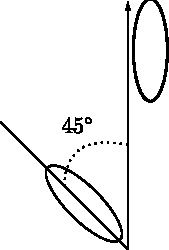
\includegraphics[scale=1]{structure/garde_pieds.pdf}
	\caption{Emplacements des pieds pour la position standard de la définition~\ref{struc:def:position-garde}.
	Le pied avant est pointé vers l'opposant, le pied arrière à \ang{45}, avec un léger écart entre les deux.
	La distance entre les deux talons est égale à la largeur des épaules.}
	\label{struc:fig:garde-pieds}
\end{figure}


\index{garde}
À noter que l'on parle parfois de garde pour cette position standard, mais il s'agit d'un abus de langage : cette position est unique et adaptée à la majorité des actions, elle sert de ligne directrice autour de laquelle le reste se construit.
En particulier cette position n'est pas défensive par elle-même puisque nous ne décrivons pas comment se protéger concrètement.
Ce n'est qu'une fois que l'on tient une arme que l'on obtient les gardes, qui sont des variantes de cette position visant chacune à protéger une partie du corps.
Nous verrons plus en détails les gardes adaptées à chaque arme au fur et à mesure.
Toutefois nous suivrons l'usage générale et ferons souvent allusion à cette position comme étant une garde, et la signification devrait être claire selon le contexte.

\noindent
Expliquons maintenant certains des points précédents :
\begin{itemize}
	\item jambes fléchies : cela permet d'abaisser le centre de gravité et d'être plus stable, et ainsi de mieux résister en cas de chocs ou de poussée (le pire étant d'avoir les jambes totalement tendues) ;
	
	\item pied avant vers l'adversaire : l'alignement du pied définit la direction d'attaque et d'avancée : ainsi si le pied pointe sur le côté, une marche entraînera du mauvais côté ;
	
	\item coudes fléchis : des coudes tendus offrent une bonne cible pour placer une clé au corps-à-corps, augmentent le risque de se faire mal aux articulations (à force de buter) et enfin diminuent la rapidité de mouvement ;
	
	\item buste de profil : cela permet d'offrir une cible plus réduite à l'opposant tout en augmentant la portée de l'arme tenue dans la main avant.
\end{itemize}
Les deux premiers éléments sont certainement parmi les plus importants.
Le lecteur est encouragé à expérimenter et à se convaincre que la position de garde proposée est celle qui propose une stabilité maximale (exercice~\ref{struc:ex:test-position} ci-dessous).

Le stabilité est importante si l'adversaire cherche à pousser ou à tirer.
De même les mouvements (pour revenir en garde, se déplacer, attaquer) seront plus rapides si les jambes sont fléchis.
Finalement la force de la frappe est augmentée si l'on peut mobiliser tout le corps, ce qui est facilité par la position décrite ci-dessus.


\begin{exercice}[Stabilité après une frappe]
	\label{struc:ex:stabilité-frappe}

	\obj{Apprendre à être stable après une frappe.}

	\begin{enumerate}
		\item \A porte une attaque dans le vide et s'arrête.
		
		\item \D attrape la main de \A et tirer pour vérifier s'il est stable.
	\end{enumerate}
\end{exercice}


En pratique la position va varier selon l'arme utilisée et le contexte.
La position que nous avons décrite est bien adaptée à la majorité des armes que nous allons étudier mais elle n'est pas universelle.
L'angle du pied arrière varie entre \ang{30} et \ang{90} selon la physiologie et l'arme employée (par exemple au corps à corps le pied aura un angle faible, et au contraire il est très grand en escrime moderne).
De même le buste sera plus de face pour de la lutte (auquel cas les pieds seront presque alignés sur un axe perpendiculaire au précédent), de profil lors d'un combat avec des armes d'estoc (avec l'escrime moderne en extrême où il n'y a pas de changement d'axe) ou encore il sera penché en avant lors de l'utilisation d'une bocle ou d'un bouclier (pour mettre les jambes hors distance).
La position est donc dictée selon des considérations physiologiques, de rapidité, de stabilité et de protection.
Nous introduirons les gardes adaptées aux différentes armes dans les chapitres traitant de celles-ci.

% Thomas
Un bon repère est d'avoir le genou au-dessus du pied, afin que le mollet soit bien vertical, tandis que la cuisse est dans l'axe du pied.
Cette position évite des douleurs aux genoux qui peuvent survenir à terme lorsque l'alignement de la jambe n'est pas correct.
De plus la distance entre les deux talons est égale à la largeur des épaules.
Cela permet de préserver les genoux et d'être plus stable.

Il n'est pas toujours facile au début de trouver la bonne position.
Le fait de se sentir à l'aise est un critère important.


\begin{exercice}[Comparaison de positions faible et forte]
	\label{struc:ex:test-position}
	
	\tags{mains nues}

	\obj{Sentir quels éléments de la position permettent à \D de résister plus facilement à la poussée de \A.}

	\A et \D travaillent ensemble.
	\D adopte une certaine position de garde, puis \A pose ses mains sur \D (épaule ou poitrine) et essaie de pousser.
	\D peut essayer de résister.
	La position adoptée par \D est variée entre les deux extrêmes :
	\begin{enumerate}
		\item \D se tient debout, jambes tendues et de face.
		\item \D adopte la garde de la définition~\ref{struc:def:position-garde}.
	\end{enumerate}

	Il n'est pas nécessaire d'y aller fort et de faire mal au partenaire : l'intérêt est plutôt de voir comment \D réagit à une poussée constante.
\end{exercice}


Lorsque deux adversaires se font face les axes définis par les pieds avant sont alignés (figure~\ref{struc:fig:garde-pieds-duel}).

\begin{figure}[ht]
	\centering
	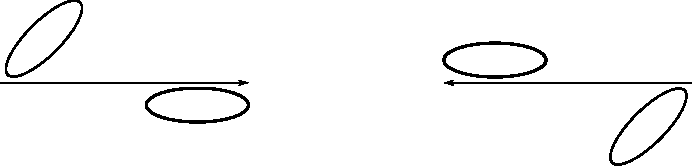
\includegraphics[scale=1]{structure/garde_pieds_duel.pdf}
	\caption{Position des pieds pour la garde standard de la définition~\ref{struc:def:position-garde}.
	L'axe des deux adversaires est aligné.}
	\label{struc:fig:garde-pieds-duel}
\end{figure}


\begin{exercice}[Structure par la lutte]
	\label{struc:ex:lutte}

	\index{echauffement@échauffement!exercice}
	\tags{échauffement \\ mains nues}

	\obj{Cet exercice travaille la structure et l'équilibre.}

	\begin{enumerate}
		\item \A et \D sont en position de garde, pied droit devant.
		De la main droite \A saisit l'intérieur du coude gauche de \D, tandis que de la main gauche il saisit l'extérieur du bras droit (haut de l'avant-bras/coude).
		\D fait de même : la position est totalement symétrique entre \A et \D.
		
		\item \A et \D se déplacent en essayant de diriger les mouvements de l'autre et en testant son équilibre.
	\end{enumerate}

	L'objectif de l'exercice est de ressentir ce qui se passe et d'utiliser les mouvements du partenaire pour le déséquilibrer et l'emmener dans la direction que l'on souhaite.
	Ainsi ce travail privilégie la sensation et non la force brute : pousser comme un barbare et serrant fort son partenaire n'a aucun intérêt.
	Voici quelques pistes pour tirer parti de cet exercice :
	\begin{itemize}
		\item Comparer la difficulté de résister en fonction de la position adoptée (que ce soit par soi-même ou par son partenaire).
		
		\item Sentir que si \A pousse dans une direction alors \D peut le déséquilibrer et augmenter l'amplitude du mouvement de \A en se dérobant et en le tirant dans la direction d'origine.
		Cela est d'autant plus efficace contre quelqu'un qui utilise la force brute.
	\end{itemize}

	Des variantes à cet exercice qui permettent de travailler le sentiment du contact sont données dans l'exercice~\ref{att:ex:lutte-variantes}.

	% \source{\cite{Kohlweiss:2014:Dijon:RingenSchwert}}
\end{exercice}


\section{Hanches}


Ainsi que nous l'avons vu plus haut, un défaut important du débutant (et qui peut perdurer longtemps) est de dissocier les différentes parties du corps.
On a souvent tendance à utiliser uniquement les bras et les épaules pour les mouvements, alors qu'un mouvement efficace mobilise le corps entier.
Les hanches sont très importantes pour unifier tout le corps, et les mouvements devraient partir de celles-ci en priorité.


\begin{exercice}[La roue (en avant)]
	\label{struc:ex:roue-avant}
	
	\tags{solitaire \\ mains nues}

	\obj{La position du corps fait qu'il est nécessaire de mobiliser les hanches lors du mouvement.}

	Dans la description de cet exercice nous donnons d'abord la position de départ, puis le mouvement qui permet d'effectuer la transition vers la position suivante, elle-même décrite dans un point séparé.
	Cette position sert alors de départ pour la transition suivante, et ainsi de suite : cet exercice est cyclique et peut être travaillé en faisant des longueurs dans le gymnase.

	\begin{enumerate}
		\item Position verticale : de face, talons joints, léger angle entre les pieds, bras tendus parallèles au corps (le gauche vers le haut, le droit vers le bas).
		
		\item Transition : avancer le pied droit en levant le bras droit vers l'avant et en basculant le bras gauche vers l'arrière.
		
		\item Position horizontale : de profil, position de profil, pieds en position de garde (jambe droite en avant), bras tendus parallèles au sol (le droit vers l'avant, le gauche vers l'arrière).
		
		\item Transition : avancer le pied gauche à côté du pied droit, le bras gauche bascule vers le bas, le bras droit se lève vers le haut.
		
		\item Position verticale (symétrique par rapport à 1.).
	\end{enumerate}

	Pendant tous l'enchaînement (en particulier dans la position verticale) les genoux sont légèrement pliés.
	Chaque partir du corps reste à la même hauteur : en particulier la tête et les épaules tracent une ligne parallèle au sol (i.e.\ le corps ne fait pas une vague en bougeant -- on retrouve cette idée dans la valse).

	Après une certaine pratique on pourra chercher à effectuer la transition dynamiquement, avec l'idée que l'on est en train d'attaquer vers l'avant.

	% \source{Échauffement en Katori Shinto Ryu.}
\end{exercice}


\begin{exercice}[La roue (en arrière)]
	\label{struc:ex:roue-arrière}
	
	\tags{solitaire \\ mains nues}

	\begin{enumerate}
		\item Position verticale : de face, talons joints, léger angle entre les pieds, bras tendus parallèles au corps (le gauche vers le haut, le droit vers le bas).
		
		\item Transition : reculer le pied gauche en levant le bras droit vers l'avant et en basculant le bras gauche vers l'arrière.
		
		\item Position horizontale : de profil, position de profil, pieds en position de garde (jambe droite en avant), bras tendus parallèles au sol (le droit vers l'avant, le gauche vers l'arrière).
		
		\item Transition : avancer le pied gauche à côté du pied droit, le bras gauche bascule vers le bas, le bras droit se lève vers le haut.
		
		\item Position verticale (symétrique par rapport à 1.).
	\end{enumerate}

	La différence avec le mouvement principale est que l'on recule le pied gauche lors du premier mouvement.
	Toutefois la position horizontale est la même que dans l'exercice précédent.

	% \source{Échauffement en Katori Shinto Ryu.}
\end{exercice}


% TODO: déplacer ailleurs
\begin{exercice}[La roue (à deux)]
	\label{struc:ex:roue-deux}

	\tags{mains nues}
	
	% on y reviendra
	\obj{Cet exercice permet de prendre conscience de l'occupation du centre de la ligne ainsi que de s'entraîner à agir en même temps que son partenaire.}

	\A et \D se font face.
	\A et \D exécutent respectivement une roue vers l'avant et une roue vers l'arrière, en simultané.

	Du fait que seul le mouvement des pieds est inversé \A et \D terminent dans une position symétrique, avec leurs bras parallèles.
	La distance entre \A et \D est de telle sorte que, en position horizontale, la main se situe au niveau de la poitrine du partenaire (sans le mouvement, le buste serait touché, l'esquive se fait parce que l'on se retrouve de profil).

	% \source{Échauffement en Katori Shinto Ryu.}
\end{exercice}


\begin{exercice}

	\tags{échauffement \\ drill}
	\index{echauffement@échauffement!exercice}
	\index{drill}

	\obj{Sentir que le mouvement des hanches est nécessaire pour enchaîner efficacement les quatre frappes.}

	\A travaille seul avec une arme quelconque~\footnotemark{}.
	\footnotetext{À ce stade les attaques et défenses n'ont pas été abordées.
	Pour cette raison le lecteur pourra ignorer cet exercice dans un premier.}

	\begin{enumerate}
		\item Départ en position de garde à gauche, pied droit devant.
		
		\item En avançant le pied gauche, monter l'épée en garde haute à gauche puis frappe à gauche à la tête.
		Léger retour en garde.
		
		\item Avancer le pied droit en attaquant en face ou à droite, retour en garde à gauche.
		
		\item Faire un demi-tour en passant le pied droit derrière, en tournant autour du côté de gauche (le talon gauche sert de point de pivot), en frappant par en dessous (l'épée est presque dans un plan perpendiculaire au sol).
		
		\item Faire un demi-tour en passant le pied droit derrière, en tournant autour du côté de gauche (le talon gauche sert de point de pivot), en frappant à droite.
	\end{enumerate}
	Cet exercice peut aussi être pratiqué en reculant : les mêmes frappes sont effectuées, mais le mouvement des jambes est inversé.

	La précision des attaques n'est pas importante au début, il vaut mieux se concentrer sur la rotation des hanches.
	Dans un second temps on pourra s'assurer que les gardes et attaques ont un sens.

	Les attaques et défenses précises doivent être adaptées en fonction de l'arme considérée.
	Voici quelques exemples :
	\begin{itemize}
		\item épée longue : 1) charrue à gauche, 2) frappe à gauche du vrai tranchant (donc en décroisant les mains) à partir d'un bœuf à gauche, 3) estoc, 4) unterhau à droite, 5) oberhau à droite ;
		
		\item mains nues : 2) direct gauche, 3) direct droit, 4) uppercut droit, 5) frappe descendante avec le talon du poing droit ;
		
		\item close combat : 2) tranche de la main droite en descendant (en revers), 3) percussion avec le talon de la paume droite, 4) percussion avec le talon de la paume droite, 5) tranche de la main droite en descendant ;
		
		\item bâton : 1) armé à gauche, 2) frappe à gauche, 3) frappe à droite, 4) frappe ascendante, 5) frappe descendante.
		
	% 	\item rapière : 1) quarte, 2) estoc puis tierce, 3) taille puis quarte, 4) estoc, 5) taille.
		
		% bokken : 1) garde de face, 2) idem que épée longue, 3) maki-uchi, 4) idem, 5) attaque via jodan
	\end{itemize}

	Il peut être intéressant de répéter l'exercice et d'avoir quelqu'un qui donne le signal pour donner un certain rythme.

	% \source{Échauffement en Katori Shinto Ryu.}
\end{exercice}


\begin{exercice}[Frappes en équilibre]

	\tags{solitaire}

	\A se met en équilibre sur une jambe et pratique n'importe quel exercice de frappe sur cible fixe.

	Dans cet exercice il est très facile de voir si \A utilise uniquement ses bras ou tout son corps pour porter ses frappes.
\end{exercice}


\section{Respiration}


Dans un premier lieu il faut savoir gérer sa respiration afin de ne pas se retrouver à court de souffle, surtout lors du combat libre et lorsqu'il fait chaud (et ce d'autant plus lorsque l'on porte un masque ou d'autres protections).
De plus le souffle permet de rythmer efficacement les mouvements, et en particulier les frappes, en expirant au moment de porter le coup.
Cette dernière idée a été particulièrement développée dans l'escrime japonaise où (presque) chaque coup est accompagnée d'un kiai.


\begin{exercice}[Frapper en expirant]

	\tags{solitaire}

	Choisir une frappe et s'entraîner à expirer en portant le coup.
\end{exercice}


\section{Résumé}


Dans ce chapitre nous avons vu que disposer d'une bonne structure est important.
En particulier les points suivants donnent des éléments pour améliorer la structure :
\begin{itemize}
	\item avoir une bonne position de garde : jambes fléchies, pied arrière à 45°, pied avant vers le partenaire, dos droit, bassin basculé ;
	\item faire attention au rôle des hanches afin d'unifier le corps ;
	\item expirer en frappant.
\end{itemize}


\chapter{Déplacements}


Savoir se déplacer est primordial en escrime : cela permet de pouvoir esquiver les attaques, augmenter l'efficacité des frappes ou encore suivre un adversaire qui s'éloigne.
Il est en effet difficile d'imaginer un combat où les deux opposants se font face sans bouger.

Bien que les déplacements ne prennent tout leur sens que lorsqu'ils sont effectués conjointement avec une autre action offensive ou défensive il reste possible d'étudier les notions principales séparément.
C'est ce que nous proposons de faire dans ce chapitre : par la suite nous reviendrons sur les déplacements en association avec les armes, et aussi sur les déplacements spécialisés associés à certains styles.

L'équilibre est une donnée primordiale lors des déplacements : toute période d'équilibre est une opportunité pour l'adversaire et doit donc être réduite au minimum, ou bien être utilisée dans un but précis.
De plus il faut garder à l'idée que l'escrime ne se pratiquait généralement pas sur une surface aussi régulière que dans un gymnase ou avec une tenue légère : les guerriers étaient amenés à combattre à l'extérieur, sur des sols inégaux (boue, dénivelé, trous…), parfois en portant des équipements (armures…).
Il est d'autant plus important de garder à l'esprit la recherche de l'équilibre afin de ne pas s'habituer aux facilités offertes.
En particulier il peut être intéressant de pratiquer en extérieur de temps en temps.


%%%%%%%%%%%%%%%%%%%%%%%%%%%%%%
\section{Déplacements simples}
%%%%%%%%%%%%%%%%%%%%%%%%%%%%%%


% TODO: images

Dans cette section tous les déplacements s'exécutent à partir de la position de garde standard (définition~\ref{struc:def:position-garde}).
De plus la majorité des déplacements terminent en garde (à l'exception de la fente).

Un point important de ne pas \emph{glisser} les pieds lorsque l'on se déplace : cela peut paraître anodin, mais en fait cela diminue la capacité de réagir.
De plus cela serait impossible sur un terrain accidenté, ou du moins dangereux (surtout si l'on porte une armure).

Les deux mouvements de base sont la marche et la retraite et permettent de progresser respectivement vers l'avant et vers l'arrière.
Dans les deux cas le mouvement est de faible amplitude -- moins de la largeur des épaules -- afin de garder l'équilibre et de pouvoir réagir rapidement (par exemple en changeant de direction).
Ainsi on préférera généralement un grand nombre de petits déplacements plutôt que quelques grandes enjambées.
Lors d'une marche c'est la jambe arrière qui pousse et qui donne l'impulsion.
Rappelons que tous ces mouvements se font avec les jambes fléchies.


\begin{definition}[Marche]
\index{déplacement!marche}

La marche correspond à un déplacement vers l'avant de faible amplitude, en avançant d'abord le pied avant suivi du pied arrière.
\end{definition}


\begin{definition}[Retraite]
\index{déplacement!retraite}
\index{déplacement!rompre|see{retraite}}

La marche correspond à un déplacement vers l'arrière de faible amplitude, en reculant d'abord le pied arrière puis le pied avant.

Le verbe correspondant est \emph{rompre}.
\end{definition}


Dans le déplacement latéral on démarre avec le pied qui se trouve du côté désiré afin de ne pas croiser les jambes (et ce quel que soit le pied avant), ce qui induirait un déséquilibre.
À noter que le pied qui se trouve à l'avant reste à l'avant à la fin du mouvement, et de même le pied à l'arrière reste à l'arrière.

% TODO: terme technique ?
\begin{definition}[Marche latérale]
\index{déplacement!marche latérale}

Dans une marche latérale vers la gauche (resp.\ droite), le pied gauche (resp.\ droit) est déplacé en premier vers la gauche (resp.\ droite), puis le pied droit (resp.\ gauche) est déplacé.
\end{definition}


Le changement de garde consiste à échanger les pieds avant et arrière.
Par exemple cela permet de se préparer à attaquer de l'autre côté ou de se défendre plus efficacement.


% marche alternée
\begin{definition}[Changement de garde avant]
\label{dep:def:changement-garde-avant}
\index{déplacement!changement de garde}
\index{garde!changement de --}

Pour un changement de garde avant le pied arrière passe à l'avant, dirigé droit devant, pendant que l'autre pied pivote pour se placer à 45°.
\end{definition}


\begin{definition}[Changement de garde arrière]

Pour un changement de garde arrière le pied avant passe à l'arrière, positionné à 45°, pendant que l'autre pied pivote pour pointer vers l'avant.
\end{definition}


% marche alternée
\begin{definition}[Changement de garde latéral]

Si le pied gauche (resp.\ droit) se trouve à l'avant, alors un changement de garde latéral à droite (resp.\ gauche) consiste à déplacer le pied droit (resp.\ gauche) vers la droite (resp.\ gauche) et en diagonale de sorte à l'amener à la même hauteur que l'autre pied, puis le pied gauche (resp.\ droit) est ramené en arrière.
\end{definition}


\begin{exercice}
\label{ex:general:miroir}

\obj{S'entraîner à réagir aux déplacements de l'adversaire.}

\A et \D se font face et se déplacent en miroir.
\end{exercice}


L'inconvénient des déplacements précédents est de ne pas permettre d'attaquer loin.
Pour ce faire on pourra utiliser une demi-fente afin de gagner en portée, en agrandissant l'écart entre les jambes.
La demi-fente est une action rapide qui s'effectue grâce à la détente de la jambe arrière.
Toutefois cette détente s'effectue au détriment de la mobilité : pour cette raison ne tendra pas totalement la jambe afin de pouvoir garder une certaine liberté de mouvement (la fente, décrite plus loin, va jusqu'au bout du mouvement).
Cela est d'autant plus vrai si l'on se trouve sur un terrain accidenté ou si l'on est alourdi par des protections.
% TODO: vérifier
% Une autre raison est que la fente totale est moins intéressante lorsqu'il s'agit de porter des coups de taille.
En particulier une fois l'attaque effectuée il faudra revenir en garde rapidement.

\begin{definition}[Demi-fente]
\label{dep:def:demi-fente}
\index{déplacement!demi-fente}

La demi-fente consiste à tendre presque entièrement la jambe arrière afin de projeter la jambe avant devant soi.
Le retour en garde se fait en poussant sur la jambe avant et en repliant la jambe arrière.
\end{definition}


\begin{definition}[Remise de fente]
\index{déplacement!remise de fente}

Après une demie-fente, la remise consiste à ramener la jambe arrière juste derrière la jambe avant afin d'exécuter une seconde fente.
\end{definition}


\begin{exercice}
\index{echauffement@échauffement!exercice}

Un meneur indique des déplacements que le reste du groupe doit effectuer : marche, retraite, fente, changement de garde.
Le rythme peut accélérer au fur et à mesure (cela fait un bon exercice d'échauffement).
\end{exercice}


Une manière de prendre l'avantage est de sortir de l'axe : cela consiste à sortir du champ d'attaque naturel de l'adversaire en se déplaçant sur le côté (par exemple avec une marche latérale).
En général ce mouvement s'accompagne d'une attaque afin de profiter d'une ligne ouverte qui sera plus difficile à l'adversaire de protéger (voir le chapitre~\ref{sec:att-def:attaque}).
Dans le cas contraire l'adversaire aura besoin de peu d'efforts pour réaligner son axe.


\begin{definition}[Sortie d'axe]
\label{dep:def:sortie-axe}
\index{déplacement!sortie d'axe}

Sortir de l'axe consiste à s'écarter de la ligne définie par la garde de l'adversaire (voir la figure~\ref{def:fig:sortie-garde}).
\end{definition}


\begin{figure}[ht]
	\centering
	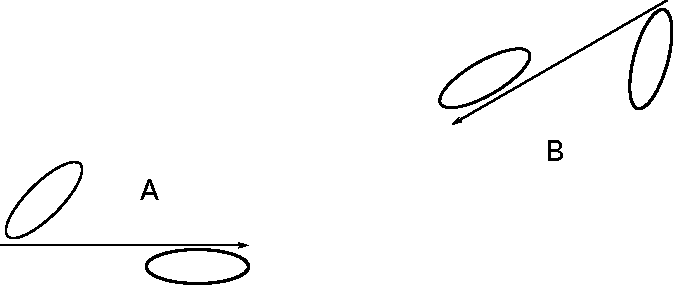
\includegraphics[scale=1]{structure/sortie_axe_pieds.pdf}
	\caption{Illustration d'une sortie d'axe.
	L'axe de B est toujours pointé vers A, mais la réciproque n'est pas vraie.}
	\label{def:fig:sortie-garde}
\end{figure}


%%%%%%%%%%%%%%%%%%%%%%%%%%%%%%%%%
\section{Déplacements techniques}
%%%%%%%%%%%%%%%%%%%%%%%%%%%%%%%%%


Les déplacements décrits dans cette section sont plus avancés et sont utilisés afin de surprendre l'adverse, que ce soit en dissimulant son intention ou en attaquant selon une ligne imprévue.
Toutefois la plupart de ces déplacements présentent une phase de déséquilibre qui peut être exploitée par l'opposant.

Nous allons maintenant décrire plusieurs mouvements, toujours de faible amplitude, qui impliquent de rapprocher les jambes ou de les croiser.
Ainsi que nous l'avons expliquer précédemment cela entraîne un certain déséquilibre, mais qui est compensé par l'ouverture de nouvelles possibilités.

En premier se trouvent les marche et retraite inversées : le pied déplacé en premier est l'inverse de celui déplacé pour une marche/retraite normale.
Dans le cas de la marche inversée l'intérêt est de pouvoir dissimuler plus longtemps le déplacement puisque la jambe arrière est moins visible tout en permettant de bénéficier d'un effet "ressort" : celui-ci peut permettre d'enchaîner efficacement avec une demi-fente au lieu d'une simple marche.
De son côté la retraite inversée peut se transformer en feinte.


\begin{definition}[Marche inversée]
\index{déplacement!marche inversée}

La marche inversée consiste à avancer d'abord le pied arrière juste derrière le pied avant, puis ensuite le pied avant.
\end{definition}


\begin{definition}[Retraite inversée]
\index{déplacement!retraite inversée}

La retraite inversée consiste à reculer d'abord le pied arrière juste derrière le pied avant, puis ensuite le pied avant.
\end{definition}


Dans les mouvements qui suivent les deux pieds se retrouvent croisés.
Ces variations se rencontrent surtout à la rapière.

% quarter du pied ?
\begin{definition}[Marche latérale croisée]
% \index{déplacement!retraite inversée}

Dans une marche latérale croisée vers la gauche (resp.\ droite), le pied droit (resp.\ gauche) est déplacé en premier vers la gauche (resp.\ droite) et dépasse le pied gauche (resp.\ droite), puis le pied droit (resp.\ gauche) est déplacé.
\end{definition}


La demi-fente est une version extrême de la demi-fente (définition~\ref{dep:def:demi-fente}) et utilisée en particulier en escrime moderne.
Son principal défaut est de limiter le mouvement et de nécessiter un certain temps pour revenir en garde du fait que les articulations sont verrouillées.


\begin{definition}[Fente]
\index{déplacement!fente}

La fente consiste à avancer largement le pied en tendant complètement la jambe arrière.
\end{definition}


% TODO: volte, balestra


%%%%%%%%%%%%%%%%
\section{Chutes}
%%%%%%%%%%%%%%%%


Dans cette section nous donnons plusieurs exercices afin de s'entraîner à tomber.
Il s'agit d'une capacité utile dans le cadre de la lutte (au corps-à-corps ou avec des armes) qui implique souvent des projections : les ignorer retire une partie des techniques disponibles et, surtout, de la réalité du combat historique (même si cela n'empêche pas de faire des projections "douces" quand son partenaire n'est pas à l'aise).
En particulier s'entraîner régulièrement permet de perdre la peur de tomber.
Finalement les chutes permettent d'ajouter un élément spectaculaire lors de des spectacles.


% Romain
\noindent
Quelques principes :
\begin{itemize}
	\item chute en avant : mettre les avants bras, ne pas tomber sur les coudes ou les genoux ;
	\item chute en arrière : remonter les épaules pour protéger la tête, se tourner un peu pour atterrir sur l'épaule et pas sur les coudes.
\end{itemize}
Une chute sur une articulation peut faire très mal si l'on porte une armure en plus.


Les trois exercices qui suivent peuvent être être effectués avec une arme (d'abord une canne, puis des armes plus lourdes et encombrantes) une fois que l'on a pris de l'assurance.


\begin{exercice}[Chute]

Se laisser tomber sur un tapis.

\end{exercice}


\begin{exercice}[Chute en hauteur]

Se laisser tomber d'un banc ou d'une table sur un tapis.

% Source : Romain.
\end{exercice}


\begin{exercice}[Roulade par dessus un obstacle]
Mettre un tapis derrière un banc et faire une roulade sur le tapis sans toucher le banc.
\end{exercice}


\begin{exercice}
\A et \D ont leur hanche droite en contact et regardent dans des directions opposées.
\A appuie et fait tomber \D en arrière.

% \source{\cite{petit:dijon:close_longword:2015}}
\end{exercice}


\begin{exercice}
\A et \D regardent dans la même direction.
\A a sa hanche gauche contre la hanche droite de \D.
\A appuie sur le torse de \D pour le faire tomber en arrière.

% \source{\cite{petit:dijon:close_longword:2015}}
\end{exercice}


\begin{exercice}
Idem que le premier exercice, mais \A mais sa jambe bien plus loin.
En général \D va tomber en avant.

% \source{\cite{petit:dijon:close_longword:2015}}
\end{exercice}


\chapter{Attaques et défenses}


% esquives


\section{Attaque}
\label{sec:att-def:attaque}

\begin{definition}[Attaques simple et composée]
\index{attaque}

\noindent
On peut distinguer les attaques simples des attaques composées :
\begin{itemize}
	\item une \emph{attaque simple} consiste en un coup isolé ;
	\item une \emph{attaque composée} (ou technique) est une séquence d'actions, chacune ayant pour objectif de préparer la suivante.
\end{itemize}
\end{definition}


Le principal intérêt d'une attaque simple est de tester l'adversaire (type de réaction, temps de réponse…) ou de le faire réagir (forcer un changement de garde…).
Des attaques simples peuvent être enchainées sans pour autant former une attaque composée : par exemple on peut induire un schéma en attaquant alternativement à gauche et à droite avec des coups de taille, pour ensuite le briser et surprendre l'adversaire.

Une attaque composée se distingue d'une attaque simple principalement par l'intention : chaque composante de l'attaque est différente et permet de préparer le terrain.
L'exemple le plus simple d'une attaque composée est une feinte sur une cible suivie d'une attaque sur une autre ouverture : si la feinte est crédible l'adversaire cherchera à se défendre contre la première attaque ce qui ouvre une autre ligne, et du fait que l'attaquant ne porte pas son coup jusqu'au bout il dispose d'une avance (en plus de l'effet de surprise).
L'idée générale est de placer l'opposant dans une situation qui le forcera à réagir d'une manière que nous pouvons exploiter : en effet face à une situation donnée il existe un certain nombre de réactions possibles (conditionnées en partie par l'arme, le style et l'expérience).
Cela explique l'intérêt d'apprendre des techniques : on dispose alors d'un vaste répertoire de pièces que nous pouvons exécuter afin de prendre l'avantage, que nous ayons pris l'initiative ou non à l'origine.
Toutefois il faut être prêt à changer son plan si l'adversaire ne réagit pas comme prévu ou si l'on perçoit une opportunité : ainsi si l'on veut exécuter une feinte mais que l'adversaire ne se protège pas alors il faut porter la frappe jusqu'au bout.

% TODO: changer de section ?

Une attaque s'accompagne d'un mouvement de jambes qui permet de donner plus de force au mouvement et de sortir de l'axe (définition~\ref{dep:def:sortie-axe}).
En effet si l'attaque se fait en avançant droit devant il y a le risque d'un coup double si l'adversaire fait de même.


\begin{coup}[Attaque directe]
\index{coup}
\index{attaque|see{coup}}

Partant d'une garde avec le pied droit (resp.\ gauche) en arrière, l'attaquant porte un coup depuis son côté droit (resp.\ gauche) en avançant le pied droit (resp.\ gauche).
\end{coup}

Le fait que le pied et l'attaque ait lieu du même côté s'expliquer par le fait que le coup est plus puissant de cette manière : dans le cas contraire, appeler contre-pied, le mouvement n'est pas naturel pour le corps (voir le commentaire dans Ringeck~\cite[p.~7]{farrell:ringeck}).
Toutefois il peut arriver que l'on souhaite attaquer du côté où se trouve le pied avant (par exemple redoubler une attaque) : dans ce cas on effectuera quand même un déplacement des pieds accompagné d'une sortie d'axe.
À noter aussi que pour certaines armes, comme l'épée longue~\cite[p.~10]{farrell:ringeck}, il est conseillé d'attaquer en premier du côté dominant car on pourra y mettre plus de force : ainsi un droitier devrait commencer par attaquer à droite, et inversement pour un gaucher.

\begin{coup}[Attaque à contre-pied]
\label{struct:coup:contre-pied}
\index{coup!en contre-pied}
\index{contre-pied}

Une attaque à contre-pied consiste à avancer le pied du côté opposé à celui où l'on attaque.
\end{coup}

Le contre-pied permet de gagner en distance et de surprendre l'adversaire.
Le gain de distance par rapport à la position normale est due à la position des épaules.


% TODO: mieux expliquer
\begin{technique}[Changement de ligne]
\label{struct:tech:changement-ligne}

\A et \D ont les lames en contact.
En tournant les mains de 180° \A peut passer derrière la lame de \D et le toucher.

Cela implique de passer de supination à pronation, ou inversement (selon le côté).

% Source : Romain.
\end{technique}


\section{Défense}


% dévier/absorber, parade franche, esquive (avec/sans couverture), reculer


\section{Concepts}


% temps
Un certain nombre de paramètres entrent en compte



\subsection{Distance}


La distance est un concept important car les techniques utilisées vont varier en fonction de celle-ci.
De plus il faut s'habituer à être capable d'évaluer rapidement les différentes distances en fonction de l'arme utilisée : être hors distance ne signifie pas la même chose quand on se bat à mains nues ou avec une lance.

Dans la définition ci-dessous nous indiquons entre parenthèses le nom allemand correspondant~\cite{kronenburg:dijon:going_distance:2015}.
L'attribution de ces mots est sujette à débat mais nous les donnons car certains les utilisent.
"Ringen" signifie "corps-à-corps", "arm" signifie "bras" et "leib" signifie "corps".
% cf Forgeng Glossary

\begin{definition}[Distances]
\index{distance}

\noindent
La distance entre deux opposants peut être définie selon les actions possibles :
\begin{itemize}
	\item \emph{hors distance} : les deux combattants sont éloignés et ne peuvent mener aucune action offensive directement ;
	
	\item \emph{approche} (zufechten) : les deux combattants sont éloignés et il suffit d'un temps pour arriver au contact des lames ;
	
	\item \emph{engagement} (fechten) : les armes des deux combattants peuvent se toucher, mais ils sont trop éloignés pour pouvoir toucher directement l'autre ;
	
	\item \emph{engagement proche} (kriegen) : les armes des deux combattants peuvent se toucher et l'opposant est à distance de touche ;
	
	\item \emph{combat rapproché} (armringen) : les deux opposants sont suffisamment proches pour pouvoir toucher l'autre en tendant le bras ou la jambe ;
	
	\item \emph{corps-à-corps} (leibringen) : les deux opposants sont très proches et peuvent travailler sur tout le corps de l'adversaire.
\end{itemize}
\end{definition}


\begin{definition}[Jeux long et court]
\index{distance!jeu court}%|textbf
\index{distance!jeu long}
\index{jeu|see{distance}}

\noindent
En escrime italienne les distances sont rassemblées de la manière suivante :
\begin{itemize}
	\item \emph{jeu long} : hors distance, approche, engagement ;
	
	\item \emph{jeu court} : engagement proche, combat rapproché, corps-à-corps.
\end{itemize}
\end{definition}

% À l'épée longue le jeu court est caractérisé par la position de \emph{mezza spada}, où les deux armes sont au contact au milieu de la lame.

La division du combat en six distances est relativement arbitraire et les frontières sont parfois floues, selon les armes et les styles.
Toutefois cela donne une première idée des actions possibles en fonction de la distance et peut servir de base au raisonnement.

Un combat débute typiquement avec les adversaires hors distance : plusieurs temps sont nécessaires avant de pouvoir lancer une attaque.
Il s'agit d'une phase d'observation où chacun essaie de se faire une idée de son opposant.
Pour cette raison les positions de garde sont peu offensives et défensives : on privilégiera des positions reposantes car l'adversaire est trop loin pour surprendre.
Il peut arriver pendant un combat que les adversaires s'éloignent pour se mettre hors distance afin de souffler.

La position devient plus hermétique dans la phase d'approche : l'adversaire est capable de porter rapidement un coup et il faut être prêt à réagir vite.
Dès qu'une attaque est portée on arrive à l'engagement : les armes sont généralement au contact afin de contrôler les mouvements de l'adversaire et de \emph{sentir} l'intention de l'adversaire.

Dès que l'engagement se rapproche il devient possible de blesser directement l'adversaire et il est donc important de ne pas perdre le contrôle et de ne pas laisser d'ouverture.
On commence aussi à disposer d'un manœuvre plus large sur l'arme de l'adversaire.
% escrime allemande
À noter que l'on passe souvent de la phase d'approche à la phase d'engagement rapproché directement : il suffit que la cible lors de l'attaque soit le corps de l'adversaire pour se retrouver très proche à la fin de l'attaque.

Finalement le combat rapproché permet de donner des coups de poing et de pied à l'adversaire.
En outre on se trouve suffisamment proche pour exécuter certaines clés sur les bras, typiquement.
Le corps-à-corps constitue la dernière étape du combat, et peut éventuellement se dérouler au sol : elle contient des saisies et des clés sur tout le corps (étranglements…) et des projections.



\subsection{Temps}




\subsection{Sentiment du contact}


\index{sentiment du fer}
Le sentiment du contact, aussi appelé plus spécifiquement le sentiment du fer, consiste à sentir l'intention de son adversaire à travers le contact que l'on a avec lui, que ce soit via les armes (bouclier compris) ou le corps.


\begin{exercice}[Variante à l'échauffement d'Ingulf]
\label{att:ex:Ingulf-variantes}
\index{echauffement@échauffement!exercice}

\obj{Cet exercice travaille la structure, l'équilibre et le sentiment du contact.}

La disposition initiale est identique à celle de l'exercice~\ref{struc:ex:Ingulf}.
Lors du déplacement des actions supplémentaires peuvent être exécutées par \A et \D afin de travailler le sentiment du contact :
\begin{enumerate}
	\item Changement de garde : \A peut passer le bras à l'extérieur (gauche au début de l'exercice) sous le bras de \D pour venir attraper l'intérieur de son coude droit.
	Cela met \A dans une position avantageuse car il contrôle totalement le centre et oblige \D à se retrouver de face, avec les deux bras à l'extérieur.
	Au combat \D possèderait peu de cibles intéressantes, à l'opposé de \A.
	
	Afin de ne pas se retrouver en position dominée \D a intérêt à changer lui aussi de garde en même temps que \A, afin de rétablir l'équilibre.
	Dans ce cas la position est exactement opposée à celle de départ.
	
	\item \A essaie d'attraper le bras de \D.
	Pour ce faire il doit lâcher sa prise et passer ses deux bras sous le bras de \D afin de le plaquer contre sa poitrine avec ses avant-bras.
	Attention aux pouces !
	L'objectif de \D est de sentir le moment où \A lâche son autre bras afin de retirer le bras ciblé.
	
	En explorant on peut remarquer que deux moments sont particulièrement adaptés : quand \D change de garde et quand \D pousse vers l'avant.
	
	\item Si \A essaie d'attraper le bras et que \D parvient à se retirer alors \D essaie de se placer dans le dos de \A et de l'enserrer avec ses bras.
	
	\item \A peut lâcher une de ses mains afin de venir toucher la tête de \D.
	\D doit sentir à quel moment \A lâche sa main afin d'esquiver en se baissant.
	
	La difficulté se trouve dans le fait que \A, à ce point de l'exercice, \A peut lâcher sa main pour exécuter différentes actions et \D doit sentir son intention.
	
	\item Fermer les yeux.
\end{enumerate}
Ces divers éléments peuvent être ajoutés un par un (en particulier la première variante est simple et devrait être ajoutée rapidement).

\source{\cite{Kohlweiss:2014:Dijon:RingenSchwert}}
\end{exercice}




\section{Exercices}


Certains des exercices peuvent se faire en plaçant un banc entre les deux partenaires.


\subsection{Mains nues}


Les exercices suivants peuvent se faire en statique ou en se déplaçant.


\begin{exercice}
\label{struct:ex:contact:frappe-signal}

\A et \D sont en garde, avant-bras en contact.
Quand \A baisse sa main, \D vient frapper à l'épaule.

Source : Romain.

\end{exercice}


\begin{exercice}

\A et \D sont en garde, avant-bras en contact.
\A donne un signal, \D vient frapper à l'épaule en enroulant un peu le bras et en gardant le contact.

Source : Romain.

\end{exercice}


\begin{exercice}
\label{struct:ex:contact:frappe-épaules}

\A et \D sont en garde, avant-bras en contact.
Quand \A le sent, il tend le bras droit pour toucher \D sur une épaule (\D ne cherche pas à se protéger).

Naturellement \A peut toucher \D à l'épaule droite juste en tendant le bras.
Mais si \A est parvenu plus dans l'intérieur de \D (par exemple en se déplaçant sur le côté plus vite, ou après un quarté du pied), alors il peut venir le toucher à l'autre épaule.

\end{exercice}


\begin{exercice}
\label{struct:ex:frappe-gauche-droite}

\A et \D se font face.

\begin{enumerate}
	\item \A frappe l'épaule gauche de \D de la main droite, en avançant la jambe droite.
	\item \D vient couvrir avec son bras droit en tournant les hanches.
	\item \A avance la jambe gauche et pose sa main gauche sur l'épaule droite de \D, en maintenant le contact avec la main droite.
\end{enumerate}

Dans l'intérêt de l'exercice, \D ne doit pas avancer sur \A.
Cet exercice est utile pour préparer certains enchaînements d'attaque droite puis gauche (e.g.
en épée longue allemande).

\end{exercice}


\subsection{Armes}


Il est intéressant de varier les armes avec lesquelles sont faits les trois exercices suivants afin de s'entraîner à estimer les distances dans divers cas.
À chaque fois l'attaque doit être normale par rapport à l'arme utilisée (ni forcée, ni exagérée, etc.).
La croix de la garde d'une épée longue (en nylon) renversée peut servir de cible.


\begin{exercice}[Mouvement dans le vide]
Effectuer des attaques simples dans le vide, puis des enchaînements.

Cet exercice devrait être un des premiers à effectuer avec toute nouvelle arme afin de s'habituer à son poids, à sa taille, aux mouvements possibles avec le corps, etc.
\end{exercice}


\begin{exercice}
\A et \D choisissent une arme quelconque.

\begin{enumerate}
	\item \A avance et s'arrête quand il se juge juste hors distance d'une attaque de \D.
	
	\item \D porte l'attaque pour vérifier.
\end{enumerate}

Source : Romain.

\end{exercice}


\begin{exercice}
\A et \D choisissent une arme quelconque.

\begin{enumerate}
	\item \A avance et \D lui dit de s'arrêter quand il le juge juste hors distance.
	
	\item \A porte l'attaque pour vérifier.
\end{enumerate}

Source : Romain.

\end{exercice}


\begin{exercice}
\A choisit une arme quelconque.

\begin{enumerate}
	\item \D avance et \A lui dit de s'arrêter quand il le juge juste à portée d'attaque.
	
	\item \A porte l'attaque pour vérifier.
\end{enumerate}

Source : Romain.

\end{exercice}


\begin{exercice}
\label{ex:frappe-dist:approche-frappe}

\begin{enumerate}
	\item \A et \D démarrent hors distance.
	\item \D s'approche de \A.
	\item Quand \A pense qu'il est à la bonne distance, il porte une frappe.
\end{enumerate}

Le but de \A est de parvenir exactement à la bonne distance pour que sa frappe soit efficace, donc ni trop près, ni hors distance.
La frappe de \A peut se faire en avançant ou en se décalant sur le côté, selon le type d'arme.
Au début on peut choisir de faire pratiquer toujours la même frappe (e.g.
un oberhau), puis ensuite de laisser le choix.
Finalement il est possible d'utiliser la croix d'une épée en nylon pour donner une cible.

\end{exercice}


\begin{exercice}
\label{ex:frappe-dist:approche-double-frappe}

Suite de l'exercice~\ref{ex:frappe-dist:approche-frappe}.

\begin{enumerate}
	\item \A et \D démarrent hors distance.
	\item \D s'approche de \A.
	\item Quand \A pense qu'il est à la bonne distance, il porte une frappe.
	\item \D recule un peu et \A porte une nouvelle attaque.
\end{enumerate}

La seconde attaque peut être soit à gauche normalement (en changeant de pied), soit en contre-pied à droite.
\end{exercice}


\begin{exercice}
\label{ex:frappe-dist:approche-croix-aleat}

La croix d'une épée nylon sert de cible.

\begin{enumerate}
	\item \A et \D démarrent hors distance.
	\item \D s'approche de \A, et à un moment décide de placer son pommeau (plus ou moins tôt) vers l'une des quatre directions nord/sud/est/ouest.
	\item Quand \A pense qu'il est à la bonne distance, il porte deux frappes consécutives dans les deux angles.
\end{enumerate}

Source : Jan.

\end{exercice}


\begin{exercice}
\label{ex:frappe-dist:approche-croix-aleat-garde}

Même exercice que \ref{ex:frappe-dist:approche-frappe}, mais juste après son coup \A doit reculer tout en revenant en garde.

Pour y parvenir \A doit être prêt à se déplacer rapidement, donc il doit être fléchi et souple pour pouvoir enchaîner les deux actions.

Cet exercice aide à préparer le combat libre.

% combat libre
\end{exercice}


\begin{exercice}
\A se met en équilibre sur une jambe et pratique n'importe quel exercice de frappe sur cible fixe.

Dans cet exercice il est très facile de voir si \A utilise uniquement ses bras ou tout son corps pour porter ses frappes.
\end{exercice}


\begin{exercice}

\begin{enumerate}
	\item \D tient l'épée horizontalement et se déplace.
	
	\item \A vient couper dessus, en essayant d'être juste limite au niveau de sa pointe.
\end{enumerate}

Si \A réussit à toucher à chaque fois alors c'est trop facile.

Source : Romain.

\end{exercice}


\begin{exercice}
\A et \D n'ont aucune protection.

\A porte une attaque et touche \D (juste un contact léger), à ce moment \D attaque \A (sans s'être protégé), et ainsi de suite.

L'idée de l'exercice est de perdre la peur d'être touché par l'arme de son équipier tout en apprenant à gérer sa force et la distance.
\end{exercice}




\chapter{Concepts généraux}


Les décisions prises lors d'un combat dépendent d'un certain nombre de paramètres que nous allons étudier dans ce chapitre.
En effet l'action juste ne sera pas la même selon la distance, les informations que nous obtenons de l'adversaire (via le contact avec son arme par exemple)


\section{Distance}


La distance est un concept important car les techniques utilisées vont varier en fonction de celle-ci.
De plus il faut s'habituer à être capable d'évaluer rapidement les différentes distances en fonction de l'arme utilisée : être hors distance ne signifie pas la même chose quand on se bat à mains nues ou avec une lance.

Dans la définition ci-dessous nous indiquons entre parenthèses le nom allemand correspondant~\cite{kronenburg:dijon:going_distance:2015}.
L'attribution de ces mots est sujette à débat mais nous les donnons car certains les utilisent.
"Ringen" signifie "corps-à-corps", "arm" signifie "bras" et "leib" signifie "corps".
% cf Forgeng Glossary

\begin{definition}[Distances]
\index{distance}

\noindent
La distance entre deux opposants peut être définie selon les actions possibles :
\begin{itemize}
	\item \emph{hors distance} : les deux combattants sont éloignés et ne peuvent mener aucune action offensive directement ;
	
	\item \emph{approche} (zufechten) : les deux combattants sont éloignés et il suffit d'un temps pour arriver au contact des lames ;
	
	\item \emph{engagement} (fechten) : les armes des deux combattants peuvent se toucher, mais ils sont trop éloignés pour pouvoir toucher directement l'autre ;
	
	\item \emph{engagement proche} (kriegen) : les armes des deux combattants peuvent se toucher et l'opposant est à distance de touche ;
	
	\item \emph{combat rapproché} (armringen) : les deux opposants sont suffisamment proches pour pouvoir toucher l'autre en tendant le bras ou la jambe ;
	
	\item \emph{corps-à-corps} (leibringen) : les deux opposants sont très proches et peuvent travailler sur tout le corps de l'adversaire.
\end{itemize}
\end{definition}


\begin{definition}[Jeux long et court]
\index{distance!jeu court}%|textbf
\index{distance!jeu long}
\index{jeu|see{distance}}

\noindent
En escrime italienne les distances sont rassemblées de la manière suivante :
\begin{itemize}
	\item \emph{jeu long} : hors distance, approche, engagement ;
	
	\item \emph{jeu court} : engagement proche, combat rapproché, corps-à-corps.
\end{itemize}
\end{definition}

% À l'épée longue le jeu court est caractérisé par la position de \emph{mezza spada}, où les deux armes sont au contact au milieu de la lame.

La division du combat en six distances est relativement arbitraire et les frontières sont parfois floues, selon les armes et les styles.
Toutefois cela donne une première idée des actions possibles en fonction de la distance et peut servir de base au raisonnement.

Un combat débute typiquement avec les adversaires hors distance : plusieurs temps sont nécessaires avant de pouvoir lancer une attaque.
Il s'agit d'une phase d'observation où chacun essaie de se faire une idée de son opposant.
Pour cette raison les positions de garde sont peu offensives et défensives : on privilégiera des positions reposantes car l'adversaire est trop loin pour surprendre.
Il peut arriver pendant un combat que les adversaires s'éloignent pour se mettre hors distance afin de souffler.

La position devient plus hermétique dans la phase d'approche : l'adversaire est capable de porter rapidement un coup et il faut être prêt à réagir vite.
Dès qu'une attaque est portée on arrive à l'engagement : les armes sont généralement au contact afin de contrôler les mouvements de l'adversaire et de \emph{sentir} l'intention de l'adversaire.

Dès que l'engagement se rapproche il devient possible de blesser directement l'adversaire et il est donc important de ne pas perdre le contrôle et de ne pas laisser d'ouverture.
On commence aussi à disposer d'un manœuvre plus large sur l'arme de l'adversaire.
% escrime allemande
À noter que l'on passe souvent de la phase d'approche à la phase d'engagement rapproché directement : il suffit que la cible lors de l'attaque soit le corps de l'adversaire pour se retrouver très proche à la fin de l'attaque.

Finalement le combat rapproché permet de donner des coups de poing et de pied à l'adversaire.
En outre on se trouve suffisamment proche pour exécuter certaines clés sur les bras, typiquement.
Le corps-à-corps constitue la dernière étape du combat, et peut éventuellement se dérouler au sol : elle contient des saisies et des clés sur tout le corps (étranglements…) et des projections.

% TODO: continuer
Une précise évaluation de la distance est nécessaire pour porter des coups précis.
Si l'adversaire est trop loin alors le coup ne portera pas, et si l'adversaire est trop proche alors nous sommes ouvert pour une contre-attaque : dans les deux cas l'adversaire peut regagner l'initiative.


\section{Temps}


\index{temps}

Une action n'est adaptée que si elle s'inscrit correctement dans le temps : trop tard et l'on s'expose à une riposte, trop tôt et l'adversaire peut se protéger et voire même prendre l'initiative.
On compte trois temps : l'avant, l'après et l'instant (ou le même-temps).
Ces temps ont été particulièrement théorisés dans la tradition de Liechtenauer, et nous indiquons la traduction allemande entre parenthèses.
En particulier il n'existe pas de mot français rendant exactement le sens de indes, donc nous utiliserons parfois les mots en allemand.


\begin{definition}[Avant (Vor)]
\index{temps!Vor}
\index{temps!avant|see{Vor}}

Agir dans l'avant signifie que l'on prend initiative (par exemple en attaquant).
\end{definition}


\begin{definition}[Après (Nach)]
\index{temps!Nachès}
\index{temps!après|see{Nach}}

Agir dans l'après signifie que l'on réagit à une action de l'adversaire.
\end{definition}


Ainsi l'un des deux adversaires va prendre l'initiative (en étant dans l'avant) tandis que l'autre devra se contenter de réagir en fonction (en étant dans l'après).
D'une certaine manière on pourrait dire que le Vor et le Nach correspondent aux actions offensives et défensives, et on pourrait penser qu'agir dans le Nach est inférieur, mais cela n'est pas tout à fait correct.
En effet il est tout à fait possible de réagir en portant soi-même une attaque, et si celle-ci est adaptée il peut même ne pas être nécessaire de se protéger.
Prenons un exemple à l'épée-bocle : \A attaque en laissant sa main à découvert (Vor), tandis que \D fait un pas sur le côté et frappe le bras (Nach).

% TODO: interpréter ce passage
% 14v-16v, p 11 : "if you cannot come in the "Before", wait for the "After"."

% ainséité / pleine conscience
Le dernier temps, Indes, joue un rôle particulier : il rejoint la notion de conscience du moment.
Il s'agit de ressentir instantanément ce qui se passe et d'agir/réagir en fonction avec la méthode la plus appropriée ; cela est particulièrement lors du liage (voir la section suivante).
Ainsi à chaque moment se situe l'Indes, et en fonction des paramètres à notre disposition on choisit d'agir dans le Vor ou dans le Nach.


\begin{definition}[Même-temps (instant, Indes)]
\index{temps!Indes}
\index{temps!instant|see{Indes}}

L'Indes consiste à être conscient des paramètres définissant le combat et à prendre une décision en conséquence.
\end{definition}


\section{Liage et sentiment du contact}


À partir du moment où l'un des deux adversaires choisit d'attaquer, la réaction de l'opposant a de fortes chances de conduire à un contact entre les deux armes : il s'agit du \emph{liage}.


\begin{definition}[Liage]
\label{conc:def:liage}
\index{liage}

Un liage est établit dès que les armes sont au contact.
\end{definition}


Le liage représente une opportunité autant qu'un danger, et de nombreuses actions décisives sont entreprises à partir du liage.
En effet on peut avoir une idée de l'intention de l'adversaire en fonction de la manière dont il manie son arme grâce au contact entre les deux armes -- le sentiment du fer.
De plus on possède alors une manière directe d'influencer l'arme, par exemple pour l'écarter.
Toutefois cette position est dangereuse et requiert une attention à chaque instant car il peut être très facile de se faire déborder, et du fait de la proximité cela signifie que l'on n'a pas de deuxième chance.
Il faut ainsi être capable de sentir précisément ce que souhaite faire l'adversaire, et de prendre la bonne décision en fonction (Indes).


\begin{definition}[Sentiment du fer]
\label{conc:def:sentiment-fer}
\index{sentiment du fer}

Le sentiment du fer (ou sentiment du contact) consiste à sentir l'intention de son adversaire à travers le contact que l'on a avec lui, que ce soit via les armes (bouclier compris) ou le corps.
\end{definition}


\begin{exercice}[Variante à l'échauffement d'Ingulf]
\label{att:ex:Ingulf-variantes}
\index{echauffement@échauffement!exercice}

\obj{Cet exercice travaille la structure, l'équilibre et le sentiment du contact.}

La disposition initiale est identique à celle de l'exercice~\ref{struc:ex:Ingulf}.
Lors du déplacement des actions supplémentaires peuvent être exécutées par \A et \D afin de travailler le sentiment du contact :
\begin{enumerate}
	\item Changement de garde : \A peut passer le bras à l'extérieur (gauche au début de l'exercice) sous le bras de \D pour venir attraper l'intérieur de son coude droit.
	Cela met \A dans une position avantageuse car il contrôle totalement le centre et oblige \D à se retrouver de face, avec les deux bras à l'extérieur.
	Au combat \D possèderait peu de cibles intéressantes, à l'opposé de \A.
	
	Afin de ne pas se retrouver en position dominée \D a intérêt à changer lui aussi de garde en même temps que \A, afin de rétablir l'équilibre.
	Dans ce cas la position est exactement opposée à celle de départ.
	
	\item \A essaie d'attraper le bras de \D.
	Pour ce faire il doit lâcher sa prise et passer ses deux bras sous le bras de \D afin de le plaquer contre sa poitrine avec ses avant-bras.
	Attention aux pouces !
	L'objectif de \D est de sentir le moment où \A lâche son autre bras afin de retirer le bras ciblé.
	
	En explorant on peut remarquer que deux moments sont particulièrement adaptés : quand \D change de garde et quand \D pousse vers l'avant.
	
	\item Si \A essaie d'attraper le bras et que \D parvient à se retirer alors \D essaie de se placer dans le dos de \A et de l'enserrer avec ses bras.
	
	\item \A peut lâcher une de ses mains afin de venir toucher la tête de \D.
	\D doit sentir à quel moment \A lâche sa main afin d'esquiver en se baissant.
	
	La difficulté se trouve dans le fait que \A, à ce point de l'exercice, \A peut lâcher sa main pour exécuter différentes actions et \D doit sentir son intention.
	
	\item Fermer les yeux.
\end{enumerate}
Ces divers éléments peuvent être ajoutés un par un (en particulier la première variante est simple et devrait être ajoutée rapidement).

\source{\cite{Kohlweiss:2014:Dijon:RingenSchwert}}
\end{exercice}


Il existe différentes manières de réagir lors du liage : soit en s'y opposant fortement et en poussant (liage fort), soit en se contentant de toucher la lame (liage faible), soit finalement en se contentant d'être présent et de sentir mais sans tomber dans les extrêmes.
La dernière approche est la meilleure car elle offre moins d'emprise à l'adversaire.
Par exemple si l'on est fort au liage l'adversaire peut facilement dérober son arme et attaquer pendant que notre arme est emportée par l'élan.
Au contraire il sera facile pour lui d'écarter notre lame (avec une percussion) si l'on ne met aucune force.
Il s'agit donc de trouver le dosage correct entre les deux.


\begin{definition}[Liage fort]
\index{liage!fort}

Un liage est dit fort si la personne pousse fermement avec son arme.
\end{definition}


\begin{definition}[Liage faible]
\index{liage!faible}

Un liage est dit faible si la personne est simplement au contact mais ne résiste pas.
\end{definition}


\section{Prendre le centre}


Une manière de demeurer protégé est de ne pas laisser d'ouvertures à l'adversaire, que l'on soit au liage ou non : il faut que chaque action qu'il entreprend ait un coût (en temps ou en sécurité).
Cela s'obtient en prenant le centre.


\begin{definition}[Prendre le centre]
\index{centre}

On parle de prendre le centre lorsque l'on occupe (avec l'arme et le corps) l'espace principal entre l'adversaire et soi-même.
\end{definition}


L'idée, en prenant le centre, est de bloquer la ligne centrale : ainsi l'adversaire ne peut attaquer directement aucune partie car il est gêné par l'arme et il s'expose à une riposte immédiate.
De plus le fait d'occuper le centre permet de menacer l'adversaire car l'on se trouve alors dans une position supérieure, avec un accès plus direct à ses ouvertures.
% important : I.33, Destreza (?), Katori


\section{Résumé}


\noindent
Les concepts importants qui ont été abordés dans ce chapitre sont :
\begin{itemize}
	\item la distance, avec la distinction entre jeu long et jeu court (propice au corps-à-corps) ;
	
	\item les temps Vor (initiative), Nach (réaction) et Indes (prise de décision en fonction des paramètres) ;
	
	\item le liage et le sentiment du fer : lorsque les armes sont au contact on peut deviner l'intention de l'adversaire et agir en fonction ;
	
	\item le centre : prendre le centre revient à établir une position forte qui bloque nos ouvertures et permet d'attaquer plus directement.
\end{itemize}


\chapter{Principes -- divers}


Nous proposons deux exercices qui permettent d'adopter facilement une garde correcte.


\begin{exercice}[Position des pieds après avoir marché]
\tags{solitaire}

\obj{Trouver la position correcte des pieds dans la position standard.}

Marcher naturellement et s'arrêter (pied droit devant).

Au moment de s'arrêter les pieds se trouvent naturellement dans une position de garde.
Il ne reste plus qu'à se baisser sur ses appuis.

\source{\cite{guidoux:dijon:thibault:2015}.}
\end{exercice}


\begin{exercice}[Trouver une bonne garde]

Se tenir pied joint, sauter en l'air et retomber jambes écartées (droite devant, gauche en arrière).

\source{\cite{enzi:dijon:messer_inner:2015}.}
\end{exercice}


\begin{exercice}
En position de garde, se pencher en avant et laisser le bras ballant du côté de la jambe arrière (type lancer de pétanque).
Grâce à un mouvement de hanches laisser le bras se balancer d'avant en arrière, puis de plus en plus vite jusqu'à faire des cercles.

% \source{\cite{enzi:dijon:messer_inner:2015}}
\end{exercice}



\part{Combat rapproché}

\chapter{Combat à mains nues}

\section{Mains nues contre couteau}

\begin{exercice}

\begin{enumerate}
	\item \A donne un coup de couteau au ventre de \D.
	
	\item \D esquive sur le côté en venant couvrir (main droite ou gauche).
\end{enumerate}

\end{exercice}



\begin{technique}

\begin{enumerate}
	\item \A donne un coup de couteau au ventre de \D.
	
	\item \D esquive sur le côté gauche et vient contrôler l'arme de la main gauche.
	\D se retrouve en garde face à \A.
	
	\item \D a plusieurs solutions pour poursuivre, par exemple :
	\begin{enumerate}
		\item frapper du poing droit dans le flanc ;
		
		\item frapper \A sous le menton avec la paume droite (passer sous son bras) ;
		
		\item tourner la tête de \A vers sa gauche en appuyant sur le côté droit de son visage avec la paume de la main droite (passer sous son bras), et passer la jambe droite derrière \A pour le projeter au sol.
	\end{enumerate}

\end{enumerate}

L'intérêt de contrôler l'arme de la main gauche est d'avoir la main droite à distance de frappe, ainsi que pour généraliser au cas où la main droite tient une arme.

Au point (3a) il est important d'engager l'épaule pour protéger le visage des coups de \A.

Source : Romain.

\end{technique}


\begin{technique}

\begin{enumerate}
	\item \A donne un coup de couteau au ventre de \D.
	
	\item \D esquive sur le côté gauche et vient contrôler l'arme de la main droite.
	
	\item \D avance sa jambe gauche et place sa main gauche dans le creux du coude (droit) de \A pour plaquer le bras contre son corps.
	
	\item \D repousse en arrière le bras de \A grâce à sa main droite, tandis que sa main gauche vient attraper son propre coude droit afin de verrouiller la prise.
\end{enumerate}

Au point (4) \D doit tenir son coude et pas autre chose : cela permet de bloquer le seul angle d'attaque où \A aurait pu frapper.

Source : Romain.

\end{technique}


\begin{technique}

\begin{enumerate}
	\item \A donne un coup de couteau au ventre de \D.
	
	\item \D saute sur le côté gauche et vient contrôler l'arme de la main droite.
	
	\item \D donne un coup de pied (droit) au ventre de \A.
\end{enumerate}

Le coup de pied au point (3) peut être exécuté plus rapidement si \D n'a pas posé le pied droit au point (2).

Source : Romain.

\end{technique}


\begin{technique}

\begin{enumerate}
	\item \A donne un coup de couteau au ventre de \D.
	
	\item \D saute sur le côté gauche et vient contrôler l'arme de la main droite.
	
	\item \D donne un coup de pied/tibia (gauche) derrière le genou droit de \A.
\end{enumerate}

Après le dernier temps \D peut profiter de sa position pour faire une clé avec sa main gauche.
L'intérêt d'avoir frapper dans le creux du genou est de pouvoir appuyer dessus pour emmener facilement \A à terre.

Source : Romain.

\end{technique}


\begin{technique}

\begin{enumerate}
	\item \A donne un coup de couteau au ventre de \D.
	
	\item \D esquive sur le côté gauche et vient contrôler l'arme de la main droite.
	
	\item \D donne frappe du poing gauche sur le flanc (droit) de \A (en avançant le pied gauche).
	En même temps il ferme sa prise avec la main droite sur le bras droit de \A.
	
	\item \D se retourne et vient percuter \A avec son épaule gauche.
	
	\item \D peut :
	\begin{enumerate}
		\item soit mettre son bras gauche en travers de la poitrine de \A et tirer avec la main droite pour faire basculer \A par-dessus son bras gauche ;
		
		\item soit attraper le bras de \A avec les deux mains et tirer.
	\end{enumerate}

\end{enumerate}

Le coup de poing et la frappe de l'épaule aux temps (3) et (4) servent à déséquilibrer \A afin de le faire tomber.
En particulier le foie se trouve vers le bas du flanc droit et fait une excellente cible.

Au point (4) \D doit veiller à garder l'arme de \A loin de lui, à un endroit où \A ne peut pas se dégager ni la retourner.

Si \A est trop grand pour être mis à terre, \D peut ramener ses mains pour lui planter son couteau dans les jambes.

Source : Romain.

\end{technique}


% TODO: coup dans le creux du genou

\chapter{Mains nues contre armes}


Dans ce chapitre nous explorons le combat à mains nues quand l'opposant est armé.
Ce type de situation est particulièrement dangereux et requiert une grande attention car l'adversaire est fortement avantagé, ne serait-ce que par la distance.


%%%%%%%%%%%%%%%%%%%%%%%%%%%%%%%%%%%
\section{Mains nues contre couteau}
%%%%%%%%%%%%%%%%%%%%%%%%%%%%%%%%%%%


% TODO: dire que la section est uniquement sur la dague, et dans la section sur le couteau; éventuellement déplacer certains dans la partie sur le close-combat

% TODO: référence au chapitre sur la dague
La majorité des techniques présentées dans cette section sont adaptées aussi à la dague qu'au couteau : l'avantage de penser aux techniques en terme de couteau oblige à se méfier du tranchant (les dagues n'étaient pas tranchantes).

Dans son traité \emph{La Fleur du combat} Fiore traite du combat à mains nue contre une dague~\cite{deiLiberi:Conan:2014:FleurCombat:Dague}.

Nous commençons par décrire des techniques générales.


\begin{exercice}

\begin{enumerate}
	\item \A donne un coup de couteau au ventre de \D.
	
	\item \D esquive sur le côté en venant couvrir (main droite ou gauche).
\end{enumerate}
\end{exercice}

% Marrozzo : accompagne le bras dans son mouvement


\begin{technique}

\begin{enumerate}
	\item \A donne un coup de couteau au ventre de \D.
	
	\item \D esquive sur le côté gauche et vient contrôler l'arme de la main gauche.
	\D se retrouve en garde face à \A.
	
	\item \D a plusieurs solutions pour poursuivre, par exemple :
	\begin{enumerate}
		\item frapper du poing droit dans le flanc ;
		
		\item frapper \A sous le menton avec la paume droite (passer sous son bras) ;
		
		\item tourner la tête de \A vers sa gauche en appuyant sur le côté droit de son visage avec la paume de la main droite (passer sous son bras), et passer la jambe droite derrière \A pour le projeter au sol.
	\end{enumerate}
\end{enumerate}

L'intérêt de contrôler l'arme de la main gauche est d'avoir la main droite à distance de frappe, ainsi que pour généraliser au cas où la main droite tient une arme.

Au point (3a) il est important d'engager l'épaule pour protéger le visage des coups de \A.

% Source : Romain.
\end{technique}


\begin{technique}

\begin{enumerate}
	\item \A donne un coup de couteau au ventre de \D.
	
	\item \D esquive sur le côté gauche et vient contrôler l'arme de la main droite.
	
	\item \D avance sa jambe gauche et place sa main gauche dans le creux du coude (droit) de \A pour plaquer le bras contre son corps.
	
	\item \D repousse en arrière le bras de \A grâce à sa main droite, tandis que sa main gauche vient attraper son propre coude droit afin de verrouiller la prise.
\end{enumerate}

Au point (4) \D doit tenir son coude et pas autre chose : cela permet de bloquer le seul angle d'attaque où \A aurait pu frapper.

% Source : Romain.
\end{technique}


\begin{technique}

\begin{enumerate}
	\item \A donne un coup de couteau au ventre de \D.
	
	\item \D saute sur le côté gauche et vient contrôler l'arme de la main droite.
	
	\item \D donne un coup de pied (droit) au ventre de \A.
\end{enumerate}

Le coup de pied au point (3) peut être exécuté plus rapidement si \D n'a pas posé le pied droit au point (2).

% Source : Romain.
\end{technique}


\begin{technique}

\begin{enumerate}
	\item \A donne un coup de couteau au ventre de \D.
	
	\item \D saute sur le côté gauche et vient contrôler l'arme de la main droite.
	
	\item \D donne un coup de pied/tibia (gauche) derrière le genou droit de \A.
\end{enumerate}

Après le dernier temps \D peut profiter de sa position pour faire une clé avec sa main gauche.
L'intérêt d'avoir frapper dans le creux du genou est de pouvoir appuyer dessus pour emmener facilement \A à terre.

% Source : Romain.
\end{technique}


\begin{technique}

\begin{enumerate}
	\item \A donne un coup de couteau au ventre de \D.
	
	\item \D esquive sur le côté gauche et vient contrôler l'arme de la main droite.
	
	\item \D donne frappe du poing gauche sur le flanc (droit) de \A (en avançant le pied gauche).
	En même temps il ferme sa prise avec la main droite sur le bras droit de \A.
	
	\item \D se retourne et vient percuter \A avec son épaule gauche.
	
	\item \D peut :
	\begin{enumerate}
		\item soit mettre son bras gauche en travers de la poitrine de \A et tirer avec la main droite pour faire basculer \A par-dessus son bras gauche ;
		
		\item soit attraper le bras de \A avec les deux mains et tirer.
	\end{enumerate}
\end{enumerate}

Le coup de poing et la frappe de l'épaule aux temps (3) et (4) servent à déséquilibrer \A afin de le faire tomber.
En particulier le foie se trouve vers le bas du flanc droit et fait une excellente cible.

Au point (4) \D doit veiller à garder l'arme de \A loin de lui, à un endroit où \A ne peut pas se dégager ni la retourner.

Si \A est trop grand pour être mis à terre, \D peut ramener ses mains pour lui planter son couteau dans les jambes.

% Source : Romain.
\end{technique}



\chapter{Dague}


La dague~\footnotemark{} que nous considérons ici n'est pas tranchante : il s'agit d'une sorte de long pic qui sert à estoquer afin de pénétrer profondément dans la peau.%
\footnotetext{Mon approche de la dague a été influencée Romain Wenz.}
Elle faisait partie de l'armement standard du combattant.
Elle fournit un moyen efficace pour continuer le combat dès que la distance est trop courte pour continuer à utiliser l'arme principale.
Elle est aussi utile pour porter un coup létal (par exemple en combat en armure, après projection au sol) car elle est beaucoup plus précise pour atteindre les cibles non protégées.
La longueur de la lame est approximativement égale à celle de l'avant-bras : cela peut servir pour se protéger l'avant-bras (un peu comme avec une tonfa) lorsque l'on combat contre une épée.
% Vadi, Fiore

\index{prise!marteau}
\index{prise!inversée}
Deux prises sont possibles pour la dague : la pointe est dirigée soit vers le haut (prise normale, ou marteau) soit vers le bas (prise inversée, ou "pic à glace").
% https://en.wikipedia.org/wiki/Icepick_grip
Typiquement la première prise correspondra à des attaques montantes tandis et la seconde à des attaques descendantes.
Les cibles respectives sont les suivantes (pour un droitier) :
\begin{itemize}
	\item prise marteau (attaques montantes, figure~\ref{dague:fig:cibles-marteau}) : abdomen gauche, aisselle gauche, sous le plexus, mains~\footnote{Les paumes ne sont pas protégées par les gantelets.} et, dans une moindre mesure, abdomen et aisselles droits ;
	\item prise inversée (attaques descendantes, figure~\ref{dague:fig:cibles-pic}) : gorge, sous le plexus, épaules gauche et droite (entre la clavicule et l'omoplate, pour atteindre le cœur) et, dans une moindre mesure, les aisselles.
\end{itemize}
Il faut appuyer de tout son corps pour bien enfoncer la lame.
Il ne faut pas juste donner de petits coups : la lame n'étant pas tranchante il n'est pas possible de blesser comme avec un couteau, et de plus chacun était formé à la lutte et pouvait ainsi parer et/ou désarmer facilement si les attaques n'étaient pas bien faites.

% video scholagladiatoria
% raisons pour prise inversée : 1) plus de force de pénétration, 2) plus pratique en combat rapproché car nécessite moins de portée (peut atteindre le dos, le cou, etc.), 3) mécanique instinctive : mouvement de haut en bas avec la main dominante, 4) plus simple de se protéger (vu qu'en général l'autre est aussi armé), sert de crochet

\begin{figure}[ht]
	\centering
	\subfloat[Prise normale.\label{dague:fig:cibles-marteau}]{\includegraphics[scale=1]{combat_rapproche/cibles_dague_marteau.pdf}}
	\hspace{3cm}
	\subfloat[Prise inversée.\label{dague:fig:cibles-pic}]{\includegraphics[scale=1]{combat_rapproche/cibles_dague_pic.pdf}}
	\caption{Cibles à la dague.}
	\label{dague:fig:cibles}
\end{figure}


\begin{exercice}[Assassins dans une rue]

Délimiter un espace sur le sol (une "ruelle") où se trouve un grand nombre de personnes, toutes armées de dague.
Certaines sont désignée comme étant des assassins par un "maître du jeu" (elles ne se connaissent pas entre elles) : leur but est d'assassiner les autres personnes, qui doivent esquiver l'attaque en faisant attention à ce qui se passe autour, et sans sortir de l'espace délimité.
\end{exercice}


\begin{technique}

\begin{enumerate}
	\item \A tient la dague en prise inversée et attaque l'épaule.
	
	\item Pied gauche en avant, le défenseur bloque en tenant sa dague horizontalement et des deux mains.
	
	\item \D attrape la main de \A avec sa main gauche, et tire vers lui en reculant le pied gauche, en essayant de le déséquilibrer
	
	\item \D avance en retournant la dague de l'ennemi contre lui-même.
\end{enumerate}
\end{technique}


\begin{technique}

\begin{enumerate}
	\item \A tient la dague en prise inversée et attaque l'épaule.
	
	\item Pied gauche en avant et en passant légèrement sur la gauche, \D bloque en tenant sa dague horizontalement et des deux mains.
	
	\item \D avance en levant les bras afin de ramener les bras de l'adversaire dans son dos et afin de les bloquer.
\end{enumerate}

Si \A résiste à la prise, alors il est avantageux de changer pour la méthode précédente.
\end{technique}


\section{Dague contre épée}


\begin{technique}

\D est armé de la dague et se tient assis.

\begin{enumerate}
	\item \A attaque à la tête.
	
	\item \D se protège en levant sa dague et en la tenant horizontalement au dessus de sa tête.
	
	\item \D se lève en baissant les bras pour écarter la lame sur sa droite (pied gauche en avant).
	
	\item \D avance pour planter la dague dans le cou de \D.
\end{enumerate}

\end{technique}


% \input{chapters/glima}


\part{Épées à une main}

\chapter{Épée à une main}


Les gardes de prime et de second sont efficaces contre les estocs et les tailles.


\begin{technique}

\begin{enumerate}
	\item \A attaque épaule ou jambe.
	
	\item \D esquive dans l'intérieur et frappe au poignet.
\end{enumerate}

% Romain
\end{technique}


\begin{technique}

\begin{enumerate}
	\item \A attaque l'épaule droite en revers.
	
	\item D pare en sixte en se déplaçant sur l'extérieur.
	
	\item \D appuie avec sa main gauche sur les mains de \A et vient frapper gorge.
\end{enumerate}

Quand il appuie \D ne doit pas retirer son épée.

% Romain
\end{technique}


\begin{technique}

\begin{enumerate}
	\item \A attaque avec un estoc.
	
	\item \D pare et ré-attaque avec un estoc.
	
	\item \A se baisse et passe en prime. 
	
	\item \A vient saisir le bras de \D et en avançant la jambe droite frappe de taille.
\end{enumerate}

Sur le dernier temps \A doit rester très près pour éviter le coup double.
Cette technique peut s'utiliser avec un bocle.

% Romain
\end{technique}


\chapter{Messer}


Le faux tranchant d'un messer est tranchant sur la toute dernière partie (\SI{10}{cm}). La prise se fait comme le sabre.
Après une attaque on casse le poignet pour étendre l'arme et trancher.
Globalement la main gauche reste en arrière.


%%%%%%%%%%%%%%%%%%%
\section{Leküchner}
%%%%%%%%%%%%%%%%%%%
\label{sec:messer:lekuchner}


Les techniques qui suivent sont similaires aux exercices~\ref{mains-nues:ex:enzi-1}, \ref{mains-nues:ex:enzi-2}, \ref{mains-nues:ex:enzi-3} et \ref{mains-nues:ex:enzi-4}.


\begin{technique}

\D démarre en garde du fou.

\begin{enumerate}
	\item \A attaque à la tête.
	\item \D recule et lève son messer pour couper sous le bras de \A avec le faux tranchant.
	\item \D revient en garde haute en reculant.
	\item \D recule encore en laissant bien son messer.
\end{enumerate}

Le but final est d'avoir un grand angle avec la direction de l'attaque afin de heurter le bras plus efficacement (sinon risque d'être parallèle à la lame).
En principe le coup est très fort, et on peut tester en visant le messer de l'autre plutôt que le bras. Pour que le pouce n'ait pas mal on abandonne la prise sabre, en le faisant glisser sur le côté.
Si \D ne revient pas en garde et qu'il a raté alors \A a la possibilité de revenir en estoc.
Fonctionne quelque soit le pied de départ et le côté où l'on part.

Source :~\cite{enzi:dijon:messer_inner:2015}.

\end{technique}


\begin{technique}

\D démarre en garde du fou.

\begin{enumerate}
	\item \A attaque à la tête.
	\item \D esquive sur le côté et coupe le poignet de \A avec le vrai tranchant.
	\item \D revient en garde haute et recule.
\end{enumerate}

La main se trouve du côté où l'on sort.

Source :~\cite{enzi:dijon:messer_inner:2015}.

\end{technique}


\begin{technique}

\D démarre en garde du fou.

\begin{enumerate}
	\item \A attaque à la tête.
	\item \D esquive sur le côté et frappe le poignet de \A avec le vrai tranchant.
	\item \D avance et appuie sur le poignet en coupant.
\end{enumerate}

Source :~\cite{enzi:dijon:messer_inner:2015}.

\end{technique}


\begin{technique}

\D démarre en garde du fou.

\begin{enumerate}
	\item \A attaque à la tête.
	\item \D pare en bœuf à gauche, en se déplaçant légèrement à gauche.
	\item De la main gauche \D pousse la main de \A un peu vers la droite.
	\item \D défend des doigts et envoie son pommeau dans la tête de \A.
	\item \D se sert du choc pour faire tourner son messer en reculant et frappe \A au visage du tranchant.
\end{enumerate}

En fait au temps 2) ce n'est pas un vrai bœuf : il s'agit juste de lever l'arme droit pour accrocher l'arme de \A dans le troisième clou.
Avant 3) \D regardait \A à droite de son bras, après 3) il le regarde à gauche.

Source :~\cite{enzi:dijon:messer_inner:2015}.

\end{technique}


\begin{technique}

\D démarre en garde du fou.

\begin{enumerate}
	\item \A attaque à la tête.
	\item \D se protège en quinte en avançant, pied gauche devant.
	\item \D heurte la main droite de \A avec sa main gauche pour écarter sa lame, tandis que de la main droite il tranche au visage.
\end{enumerate}

Le mouvement en 2) est l'éternel écartement des épaules cher à Romain.
En 3) Enzi conseille de reculer.

Le mouvement du corps est le même que l'exercice~\ref{mains-nues:ex:enzi-2}.

Source :~\cite{enzi:dijon:messer_inner:2015}.

\end{technique}


\begin{technique}

\D démarre en garde du fou.

\begin{enumerate}
	\item \A attaque à la tête.
	\item \D se protège en quinte en avançant, pied gauche devant.
	\item Du tranchant de la main \D percute l'avant bras de \A.
	\item \D ramène son bras gauche, en accrochant éventuellement le pommeau de \A, et pousse avec le bras droit pour écraser le messer de \A et trancher au visage de \A.
\end{enumerate}

Il est important de ne pas chercher à saisir le pommeau : le placement est tel que le messer adversaire sera soit hors portée, soit retenu par la main. Le coup se fait entre le poignet et le coude.
Au dernier temps \A va en général se faire trancher aussi par le faux tranchant de sa propre arme.
% TODO: Le mouvement d'écartement est toujours celui de Romain.

Source :~\cite{enzi:dijon:messer_inner:2015}.

\end{technique}


\begin{technique}

\D n'a pas d'arme.

\begin{enumerate}
	\item \A attaque à la tête.
	\item \D part sur la gauche et couvre avec son bras droit, main vers le haut.
	\item \D éjecte le bras de \A avec un mouvement circulaire dans le sens horaire.
	\item \D frappe \A.
\end{enumerate}

L'objectif au temps 2) est de parvenir à arriver avec l'avant-bras contre le plat de la lame.
Voir l'exercice~\ref{mains-nues:ex:enzi-4}.

Source :~\cite{enzi:dijon:messer_inner:2015}.

\end{technique}



% \input{chapters/sabre_abordage}


\part{Épée longue}

\chapter{Épée longue}

\section{Général}

\begin{technique}

\begin{enumerate}
	\item \A attaque à l'épaule droite.
	
	\item \D se déplace sur le côté gauche et absorbé en tierce.
	
	\item \D passe sa jambe droite vers la gauche et frappe À avec un coup montant.
	
	\item \A monte en bœuf pour se défendre.
\end{enumerate}

Cette technique travaille le contre-pied, et les défenses rapides pour \A.

Source : Romain.

\end{technique}


\begin{technique}
\begin{enumerate}
	\item \A et \D sont en garde, pied gauche en avant.
	
	\item \A attaque l'épaule gauche de \D (sur une diagonale) en avançant le pied droit.
	
	\item \D s'esquive et utilise son épée pour écarter l'épée de \A (dans la direction où elle allait).
	
	\item \A utilise l'élan fournit par le chassé de \D afin de reculer le pied droit et de passer dans la garde du bœuf (à droite).
	
	\item \D essaie de se de déplacer pour estoquer.
	
	\A doit viser au niveau de l'épaule droite de \D, s'il est plus haut, \D peut facilement passer en-dessous. De plus \A doit être vraiment fléchi et ferme, en mettant son épée bien devant lui pour occuper le centre.
	
	\item \A ramène son pied gauche derrière le droit pour amener la pointe de son épée au niveau du ventre de \D.
	
	Ce dernier mouvement ne peut être bien accompli que si \A est bien fléchi, ce qui lui permet de changer de direction facilement et de réagir vite.
\end{enumerate}

Cette technique est symétrique.

Source : Romain (CdA).
\end{technique}

\section{Liechtenauer (allemande)}

La référence pour l'escrime de Liechtenauer est le tétraptyque des quatre glossateurs, traduit par l'\textsc{Ardamhe}~\cite{ardamhe:tetraptyque}.

En épée longue allemande, le corps est divisé en quatre quadrants, et à chacun correspond une cible qui peut être attaquée avec un coup ascendant ou descendant.

Après chaque attaque il est important de finir dans une garde :
\begin{itemize}
	\item une attaque descendante termine dans la garde de la charrue ;
	\item une attaque ascendante termine dans la garde du bœuf.
\end{itemize}
Les attaques de base se font sur les diagonales, donc si l'attaque démarre à gauche, la garde sera du côté droit, et inversement.

\subsection{Exercices généraux}

Les deux techniques suivants sont utiles pour gagner en fluidité au niveau des poignets, sur les attaques descendantes et ascendantes. Ils peuvent se faire dans le vide, ou avec un partenaire légèrement hors distance.

\begin{exercice}

\begin{enumerate}
	\item \A commence pied gauche en avant.
	\item \A frappe en diagonale droite.
	\item Quand son arme a dépassé le flanc de \D, \A ramène sa main droite en arrière et tourne le poignet gauche, de manière à croiser les poignets avec la lame vers l'arrière.
	\item \A lève les bras et attaque sur la diagonale inverse.
	\item Quand l'arme a dépassé le flanc de \D, \A tourne les deux poignets pour amener l'épée sur le côté.
\end{enumerate}

Au dernier point \A n'a plus qu'à lever les mains pour se retrouver dans la position de départ. L'intérêt de l'technique est d'enchaîner rapidement plusieurs séries.

Source : CdA.
\end{exercice}


\begin{exercice}
Cet exercice est exactement comme le précédent mais avec des attaques ascendantes sur les diagonales. Cette fois-ci les poignets ne sont pas croisés à gauche, mais croisés à droite.

Source : CdA.
\end{exercice}


\begin{technique}

\begin{enumerate}
	\item Départ pieds gauches en avant, \A lance un coup furieux qui est tout juste à la bonne distance.
	\item \D porte son poids sur la jambe arrière pour laisser passer court.
	\item \D passe le pied droit devant et attaque droit devant.
\end{enumerate}

Si le furieux était fait plus proche, alors il faudrait parer avec un furieux en allant sur le côté, mais ici comme le coup peut passer court il est plus économique de procéder ainsi.

Pour que le coup passe il faut que le coup de \D soit franc et termine la pointe loin sur le côté (pas menaçant d'estoc).

Finalement une variante est la suivante : \A avance le pied droit mais sans attaquer. Dans ce cas \D doit attaquer directement. Une manière de savoir si \A attaque ou non est de surveiller les hanches (plutôt que de regarder à la fois les jambes et les bras) : si \A attaque elles seront bien positionnées, sinon elles seront vrillées.

Cette technique peut se faire sur celui du miroir (ex.~\ref{ex:general:miroir}).
\end{technique}


% TODO: techniques séparés
\begin{technique}
Dans cet technique nous allons étudier les coups de maître comme des brisures de garde :
\begin{itemize}
	\item \D en garde du fou : coup crânien~\footnote{Sans masque le faire légèrement hors distance et menacer la poitrine.} ;
	\item \D en garde de la charrue ou en longue pointe : coup bigle ;
	\item \D en garde du bœuf : coup tordu~\footnote{Sans gants le faire sur le fort de la lame, en principe on vise les doigts.} ;
	\item \D en garde du jour : coup de travers.
\end{itemize}
La longue pointe peut aussi briser toute les gardes.

Note sur le coup tordu : il est important de le faire en croisant les poignets (pour \D en bœuf du côté gauche), et non pas en faisant un coup furieux, car dans ce dernier cas nous n'occupons plus le centre et l'autre peut facilement changer sa lame de côté. Avec les poignets croisés, on est vraiment face à l'adversaire, et on est plus offensif même si l'épée est sur le côté (il est possible de la ramener rapidement vers le centre).

De même on doit faire le coup tordu du même côté que la garde de \D (donc sortir à droite si \D est en garde à sa gauche), car sinon on n'occupe pas le centre et \D peut estoquer à la cuisse.

\begin{figure}[ht]
	\centering
	\includegraphics[scale=1]{epee_longue/coup_cranien}
	\caption{Schéma de déplacement pour le coup crânien. Quand \A est sur le cercle, il se trouve hors distance par rapport à \D situé au centre. En sautant sur une ligne droite entre deux points du cercle, \A se retrouve, au milieu de son segment, à un endroit où il peut atteindre \D, et c'est à cet endroit qu'il porte le coup. Diagramme dû à Thomas.}
\end{figure}

Source : Raphaël (CdA).
\end{technique}


\subsection{Le coup furieux (Zornhau) et ses pièces}

\begin{coup}[Coup furieux – \emph{Zornhau}]
Le coup furieux (all. \emph{Zornhau}, ang. \emph{wrath strike}) est le coup de maître le plus simple.
Il consiste à avancer le pied arrière en portant un coup diagonal au niveau de l'épaule~\cite[fol.~19r-20v, p.~16]{farrell:ringeck}.
Si le coup n'a pas touché la cible, la pointe est menaçante, à hauteur de la poitrine ou du visage.
\end{coup}

Noter qu'à la fin l'attaquant ne se trouve pas en fente.
De plus les mains ne doivent pas être trop hautes (à peu près à la hauteur du nombril – pour le coup "normal").


\begin{technique}

\begin{enumerate}
	\item \A porte un coup furieux en restant sur la même ligne.
	
	\item En réaction \D porte aussi un coup furieux mais en se décalant sur le côté.
	La pointe de l'épée est dirigée vers le visage de \A.
\end{enumerate}

À la fin du temps (2), l'épée de \D se trouve alignée avec la ligne qui joignait originellement \A et \D.
Pour cette raison \D se trouve dans une position bien plus forte.
Cela montre l'intérêt de se décaler lors de l'attaque, et l'technique suppose que \A est naïf.

Source : Raphaël (CdA), d'après~\cite[fol.~19r-20v, §1, p.~16]{farrell:ringeck}.
\end{technique}


\begin{technique}

\begin{enumerate}
	\item \A porte un coup furieux en se décalant sur le côté.
	
	\item En réaction \D porte un coup furieux en se décalant sur le côté.
	
	\item Si \A résiste, \D se baisse pour passer sous l'épée de \A et fait une fente sur la gauche.
	En même temps il fait glisser son épée le long de l'épée de \A (vers soi), la fait passer de l'autre côté et porte une attaque en finissant 
\end{enumerate}

L'attaque au point (3) peut se faire selon la même diagonale que la première attaque (temps (2)), ou bien sur la diagonale opposée.
Il est important de toujours garder le contact avec l'épée de \A, et de ne jamais mettre son épée en arrière.
En principe \D n'a pas le temps de décaler la jambe droite pour revenir d'une vraie garde, mais il doit le faire dès que possible pour redevenir stable.

Contrairement à l'technique précédent la position au temps (2) est symétrique car \A et \D se sont tous les deux décalés.
Pour cette raison les rôles peuvent être inversés au point (3) (\A peut attaquer s'il sent une résistance de la part de \D).

Cette attaque est à utiliser dès que l'on sent une forte résistance de la part de l'opposant.
Celle-ci donne alors le point de pivot nécessaire.

Source : Raphaël (CdA), d'après~\cite[fol.~19r-20v, §2, p.~16]{farrell:ringeck}.
\end{technique}


\begin{technique}

\begin{enumerate}
	\item \A porte un coup furieux en se décalant sur le côté.
	
	\item En réaction \D porte un coup furieux en se décalant sur le côté.
	
	\item \D lève les mains (soit dos de la main droite vers le haut – en bœuf – soit paume en haut) pour menacer la poitrine de \A.
	
	\item \A lève son épée verticalement dans un mouvement réflexe pour se protéger.
	
	\item \D contourne la garde et les bras de \A avec la pointe de son épée pour venir estoquer la poitrine, entre les bras.
\end{enumerate}

Cette technique est à utiliser quand aucun des deux opposants n'exerce de pression.
La réaction de \A au point (4) est mauvaise, la technique suivante montre la réponse correcte.

L'avantage de monter en bœuf au point (3) est d'offrir plus de possibilités si \A réagit (par exemple en enchaînant avec un coup de travers).
L'autre position est plus rapide à exécuter, mais il vaut mieux l'exécuter si \A ne pourra pas réagir.
Une fois les mains levées il s'agit d'une vraie garde (quillons environ horizontaux, etc.).
A priori le faible de \A se trouve accroché dans la garde.

Encore une fois cette technique est symétrique à partir du point (2).

Source : Raphaël (CdA), d'après~\cite[fol.~19r-20v, §3–4, pp.~16–17]{farrell:ringeck}.
\end{technique}


\begin{technique}[Mutation]

\begin{enumerate}
	\item \A porte un coup furieux en se décalant sur le côté.
	
	\item En réaction \D porte un coup furieux en se décalant sur le côté.
	
	\item \D lève les mains (soit dos de la main droite vers le haut – en bœuf – soit paume en haut) pour menacer la poitrine de \A.
	
	\item \A lève son épée verticalement pour placer son fort contre le faible de \D puis il ramène son épée vers le sol en gardant la pointe de \D dans sa garde. \A change de garde car \D pourrait estoquer dans la jambe à l'avant.
	
	\item \A peut estoquer la jambe de \D.
\end{enumerate}

Une mutation consiste à prendre le faible adverse dans son propre fort, et à amener sa pointe vers une cible (haute si on était bas avant, et inversement).

Source : Raphaël (CdA), d'après~\cite[fol.~23v-24v, §3, p.~23]{farrell:ringeck}.
\end{technique}

% Krumphau
% deux versions : en rapproché, coup doux pour venir prendre le liage (et si la distance est un peu plus grande on peut venir couper sur la lame) ; de loin (par exemple ouverture d'un combat) : coup puissant (avec un grand saut) car on ne sait pas ce que l'autre va faire et on veut juste virer son épée dans tous les cas

\section{Italienne}

% poids typique : 1.7 kg

% Romain
Les parades se font toujours en se déplaçant sur le côté afin d'adoucir le choc : les épées étant lourdes il n'est pas possible de prendre une parade franche sans se déplacer.

% Romain
Une attaque peut être précédée d'un batté.
Ce batté peut envoyer l'épée dans la même direction que celle du déplacement, mais la position de l'attaque est telle que le défenseur ne peut pas revenir.

% Romain
L'escrime italienne à l'épée longue se fait typiquement en armure de plates.
Sur une amure trois zones absorbent très bien les chocs du fait de la largeur de la plaque de métal : les avant-bras et bras, les cuisses et le ventre (côtés compris).
Il est donc possible de rabattre volontairement l'arme adverse sur ces zones, cf les trois premiers techniques.
Cela provoque un effet de surprise, et de plus l'opposant perd l'amplitude qui donne de la force à sa frappe, ce qui augmente l'intérêt d'avancer vraiment.

% Romain
Quand la distance est faible et que l'on tient l'épée à une main, il faut avoir le dos de la main sur le dessus (pronation).
En effet si la lame est chassée dans cette position il sera beaucoup plus facile de revenir que si la main est tournée dans l'autre sens.

% Romain
Si \A et \D ont le fer en contact et que \A ne menace pas \D avec sa pointe en la gardant bien entre les deux, \D peut tourner ses poignets d'un côté en se déplaçant dans la même direction, ce qui permet d'estoquer.
Par exemple si son l'épée est placée pour attaquer l'épaule gauche de \A, \D tourne ses mains dans le sens anti-horaire – avec la main droite passant de supination à pronation – et va vers la droite.
De même si \A essaie de faire une entrée en lutte alors qu'il se trouve trop loin il est possible d'utiliser cette technique.


\begin{coup}[Estramaçon]
L'estramaçon est un grand coup donné verticalement avec le tranchant.
\end{coup}


\begin{technique}

\begin{enumerate}
	\item \A attaque depuis sa droite l'épaule gauche de \D.
	\item \D pare en quarte en se déplaçant sur le côté droit.
	\item \D lâche sa main gauche et vient heurter la lame de \A avec son avant-bras (par-dessus) pour la rabattre sur son bras, en changeant de jambe.
	\item \D tourne sa main en pronation et vient placer sa main gauche sous la lame.
\end{enumerate}

Au point (3) il est important que \D s'accroupisse très bas et entre dans la distance.
De plus \D doit prendre garde à toujours garder sa pointe menaçante, bien au centre.

Source : Romain, d'après Fiore.

\end{technique}


\begin{technique}

\begin{enumerate}
	\item \A attaque depuis sa droite l'épaule gauche de \D.
	\item \D pare en quarte en se déplaçant sur le côté droit.
	\item \D lâche sa main gauche et vient passer son bras entre les deux lames, pour ensuite enrouler son bras autour de la lame, en changeant de jambe. \D attrape le quillon (du bas) de \A.
\end{enumerate}

Cette technique est moins efficace que la technique précédente.
Il est important de tenir le quillon car sinon \A peut dégager sa lame en tirant dessus, et en profiter pour couper sous l'aisselle (sauf si \D est suffisamment près et menaçant avec sa pointe).

Source : Romain, d'après Fiore.

\end{technique}


\begin{technique}

\begin{enumerate}
	\item \A attaque depuis sa droite l'épaule gauche de \D.
	\item \D pare en quarte en se déplaçant sur le côté droit.
	\item \D pose sa paume gauche sur le plat de sa lame et s'en sert pour venir abattre la lame de \A contre sa cuisse (à \D).
\end{enumerate}

L'intérêt de poser sa main sur sa propre lame est de ne pas prendre le risque d'attraper le tranchant de \A.

Source : Romain, d'après Fiore.

\end{technique}


\begin{technique}

\begin{enumerate}
	\item \A attaque depuis la droite.
	\item \D pare en quarte puis monte en bœuf (mutation) pour estoquer.
	\item \A lève les mains, fait faire un tour avec son épée derrère lui et vient frapper derrière le genou droit de \D en faisant un grand saut sur le côté.
\end{enumerate}

L'idée pour \A est de finir juste à porter du genou, qui est situé un peu devant l'épaule, et ainsi \D est trop loin pour frapper.
Le coup doit arrivée derrière le genou car le côté est protéger par des disques de métal.

Le coup en (3) est l'équivalent italien d'un Zwerchau, qui est beaucoup plus ample.

Source : Romain, d'après Marozzo.

\end{technique}


\begin{technique}

\begin{enumerate}
	\item \A attaque depuis sa droite.
	\item \D pare en quarte.
	\item \D vient en seconde.
	\item \D peut venir piquer la jambe ou, mieux, venir frapper au visage avec le faux tranchant.
\end{enumerate}

\end{technique}


\begin{technique}

\begin{enumerate}
	\item \A attaque avec un estoc.
	\item \D pare en quarte.
	\item \D chasse l'épée de \A vers la droite avec le faux tranchant et il finit en octave.
	\item \D laisse son épée aller en arrière et profite de l'élan pour venir frapper.
\end{enumerate}

Un bon estoc se fait en laissant d'abord tomber l'épée horizontalement, et ensuite en poussant la pointe.
Le pied se pose juste après l'impact, ce qui permet de pouvoir continuer d'avancer si l'autre recule.
Cette manière de faire est aussi plus précise.
% ça diminue le chance de coup double car l'autre voit que \A a décidé de prendre l'initiative

Au point (3) \D peut attendre que \A décide d'avancer/reculer, ou bien encore qu'il relâche un peu sa menace, pour lancer la suite.

Source : Romain.

\end{technique}


Les trois techniques qui suivent sont efficaces contre un adversaire qui cherche à avoir la tête, et en particulier en combat libre où il y a de nombreux coups doubles.
Au dernier temps la position de la lame empêche \A de pouvoir toucher \D.
Dans tous les cas, au moment de la parade, \D doit maintenir sa pointe en direction du visage de \A pour garder le contrôle du centre.
Ainsi si \A recule \D peut le suivre facilement, et \A ne peut pas non plus attaquer.


\begin{technique}

\begin{enumerate}
	\item \A attaque \D sur son épaule droite.
	
	\item \D pare avec le faux tranchant (en sixte).
	
	\item \D avance en diagonale vers la gauche et vient frapper \A avec le vrai tranchant.
\end{enumerate}

Source : Romain, d'après Marozzo.

\end{technique}


\begin{technique}

\begin{enumerate}
	\item \A attaque \D sur son épaule droite ou sur la tête.
	
	\item \D pare avec le faux tranchant (en quinte, pointe vers la gauche).
	
	\item \D avance en diagonale vers la gauche et vient frapper \A à la tête avec le vrai tranchant, l'épée totalement dans l'axe.
\end{enumerate}

Source : Romain, d'après Marozzo.

\end{technique}


\begin{technique}

\begin{enumerate}
	\item \A attaque \D sur son épaule gauche.
	
	\item \D pare avec le vrai tranchant (en quarte).
	
	\item \D avance en diagonale vers la droite et vient frapper \A avec le faux tranchant.
\end{enumerate}

Source : Romain, d'après Marozzo.

\end{technique}


\begin{technique}[Coup de travers italien]

\begin{enumerate}
	\item \A menace \D dans le cadrant supérieur droit en passant en bœuf.
	
	\item \A déplace son pied gauche loin sur le côté mais en gardant son buste et son épée aux mêmes endroits.
	
	\item \A décroche son épée et exécute un coup de travers en ramenant son pied arrière, en ciblant l'arrière de la jambe de \D.
\end{enumerate}

Le fait de déplacer le pied gauche sans le reste du corps induit une torsion qui va donner la force au coup en rotation.

La première menace permet de fixer l'épée adverse, et il faut donc l'encourager à rester de ce côté en menaçant vraiment, sinon dès qu'il sentira que l'épée décroche il pourra revenir prendre le centre facilement.

Source : Romain, d'après Marozzo.
\end{technique}


\begin{technique}

\begin{enumerate}
	\item \A et \D démarre en longue pointe.
	
	\item \A donne un coup vertical en visant la tête.
	
	\item \D se décale sur le côté et frappe en diagonale pour intercepter la lame de \A tout en le frappant à la tête.
\end{enumerate}

Comme \D se décale en second il a un léger avantage au niveau de l'axe.
La frappe de \D doit être diagonale pour briser la symétrie : si elle était aussi verticale alors il pourrait y avoir un coup double.

Source : Romain.
% travail avec un boken pour mieux sentir
\end{technique}


\chapter{Épée longue allemande -- Liechtenauer}
\label{chap:épée-longue-liechtenauer}


Le texte original de Liechtenauer, appelé le Zettel, est particulièrement cryptique.
Heureusement le texte a été analysée par quatre glossateurs: Sigmund Ringeck, Peter von Danzig, Juden Lew, Hans von Speyer.
Ces quatre textes ont été regroupés en français dans le tétraptyque~\cite{Liechtenauer:Ardamhe:2010:Tetraptyque}.
Une excellente traduction (anglaise) du Ringecka été compilée par Keith Farrell~\cite{Ringeck:Farrell:2014:CodexRingeck}.


\section{Concepts généraux}


% TODO: winden, schnappen, duplieren, zucken
% coup de maîtres
% http://www.amheonweb.net/forum/viewtopic.php?f=7&t=535


En épée longue allemande, le corps est divisé en quatre quadrants, et à chacun correspond une cible qui peut être attaquée avec un coup ascendant ou descendant.

Après chaque attaque il est important de finir dans une garde :
\begin{itemize}
	\item une attaque descendante termine dans la garde de la charrue ;
	\item une attaque ascendante termine dans la garde du bœuf.
\end{itemize}
Les attaques de base se font sur les diagonales, donc si l'attaque démarre à gauche, la garde sera du côté droit, et inversement.
Ces attaques ont déjà été décrites auparavant, mais nous les rappelons en les décrivant d'une autre manière afin de les replacer dans le contexte de l'escrime allemande.


\begin{coup}[Oberhau (coup supérieur)]
\label{épée-longue:coup:oberhau}
\index{coup!allemand!oberhau}
\index{oberhau|see{coup allemand}}

Un oberhau est un coup descendant à partir d'une garde haute (voir coup~\ref{att:coup:descendant}).
\end{coup}


\begin{coup}[Unterhau (coup inférieur)]
\label{épée-longue:coup:unterhau}
\index{coup!allemand!unterhau}
\index{unterhau|see{coup allemand}}

Un unterhau est un coup ascendant à partir d'une garde basse (voir coup~\ref{att:coup:montant}).
\end{coup}


\begin{coup}[Mittelhau (coup intermédiaire)]
\label{épée-longue:coup:mittelhau}
\index{coup!allemand!mittelhau}
\index{mittelhau|see{coup allemand}}

Un mittelhau est un coup horizontal (voir coup~\ref{att:coup:latéral}).
\end{coup}


L'oberhau et l'unterhau sont des termes génériques.
En général si aucune indication plus précise n'est donnée il s'agit d'une frappe diagonale : par exemple si l'on est en garde haute avec l'épée au niveau de l'épaule droite, alors un oberhau consistera en une frappe sur la diagonale droite.


\begin{garde}[Versetzen]
\index{versetzen}

Le versetzen est un simple mouvement de défense en opposant sa lame au coup.
\end{garde}


\section{Exercices généraux}


Les deux techniques suivants sont utiles pour gagner en fluidité au niveau des poignets, sur les attaques descendantes et ascendantes. Ils peuvent se faire dans le vide, ou avec un partenaire légèrement hors distance.

\begin{exercice}

\begin{enumerate}
	\item \A commence pied gauche en avant.
	\item \A frappe en diagonale droite.
	\item Quand son arme a dépassé le flanc de \D, \A ramène sa main droite en arrière et tourne le poignet gauche, de manière à croiser les poignets avec la lame vers l'arrière.
	\item \A lève les bras et attaque sur la diagonale inverse.
	\item Quand l'arme a dépassé le flanc de \D, \A tourne les deux poignets pour amener l'épée sur le côté.
\end{enumerate}

Au dernier point \A n'a plus qu'à lever les mains pour se retrouver dans la position de départ. L'intérêt de la technique est d'enchaîner rapidement plusieurs séries.

% Source : CdA.
\end{exercice}


\begin{exercice}
Cet exercice est exactement comme le précédent mais avec des attaques ascendantes sur les diagonales. Cette fois-ci les poignets ne sont pas croisés à gauche, mais croisés à droite.

% Source : CdA.
\end{exercice}


% TODO: comprendre
% \begin{exercice}
% Placer les pieds sur une ligne horizontale, écartés confortablement.
% En partant d'une garde, porter un coup et finir dans la garde opposée.
% 
% Les combinaisons sont les suivantes :
% \begin{itemize}
% 	\item garde du toit et oberhau ;
% 	\item garde du toit et unterhau ;
% 	\item garde du bœuf et estoc ;
% 	\item garde de la charrue et estoc.
% \end{itemize}
% 
% L'intérêt de l'exercice est de forcer à bouger les hanches.
% 
% Source : \cite{kronenburg:dijon:going_distance:2015}.
% \end{exercice}


\begin{technique}

\begin{enumerate}
	\item Départ pieds gauches en avant, \A lance un coup furieux qui est tout juste à la bonne distance.
	\item \D porte son poids sur la jambe arrière pour laisser passer court.
	\item \D passe le pied droit devant et attaque droit devant.
\end{enumerate}

Si le furieux était fait plus proche, alors il faudrait parer avec un furieux en allant sur le côté, mais ici comme le coup peut passer court il est plus économique de procéder ainsi.

Pour que le coup passe il faut que le coup de \D soit franc et termine la pointe loin sur le côté (pas menaçant d'estoc).

Finalement une variante est la suivante : \A avance le pied droit mais sans attaquer. Dans ce cas \D doit attaquer directement. Une manière de savoir si \A attaque ou non est de surveiller les hanches (plutôt que de regarder à la fois les jambes et les bras) : si \A attaque elles seront bien positionnées, sinon elles seront vrillées.

Cette technique peut se faire sur celui du miroir (ex.~\ref{ex:general:miroir}).
\end{technique}


% TODO: techniques séparés
\begin{technique}
Dans cette technique nous allons étudier les coups de maître comme des brisures de garde :
\begin{itemize}
	\item \D en garde du fou : coup crânien~\footnote{Sans masque le faire légèrement hors distance et menacer la poitrine.} ;
	\item \D en garde de la charrue ou en longue pointe : coup bigle ;
	\item \D en garde du bœuf : coup tordu~\footnote{Sans gants le faire sur le fort de la lame, en principe on vise les doigts.} ;
	\item \D en garde du jour : coup de travers.
\end{itemize}
La longue pointe peut aussi briser toute les gardes.

Note sur le coup tordu : il est important de le faire en croisant les poignets (pour \D en bœuf du côté gauche), et non pas en faisant un coup furieux, car dans ce dernier cas nous n'occupons plus le centre et l'autre peut facilement changer sa lame de côté. Avec les poignets croisés, on est vraiment face à l'adversaire, et on est plus offensif même si l'épée est sur le côté (il est possible de la ramener rapidement vers le centre).

De même on doit faire le coup tordu du même côté que la garde de \D (donc sortir à droite si \D est en garde à sa gauche), car sinon on n'occupe pas le centre et \D peut estoquer à la cuisse.

% Source : Raphaël (CdA).
\end{technique}


% TODO: principe valable plus généralement
% TODO: ne peut pas être inclus dans le théorème
\begin{figure}[ht]
	\centering
	\includegraphics[scale=1]{epee_longue/coup_cranien}
	\caption{Schéma de déplacement pour le coup crânien. Quand \A est sur le cercle, il se trouve hors distance par rapport à \D situé au centre. En sautant sur une ligne droite entre deux points du cercle, \A se retrouve, au milieu de son segment, à un endroit où il peut atteindre \D, et c'est à cet endroit qu'il porte le coup. Diagramme dû à Thomas.}
\end{figure}



\section{Le coup furieux (Zornhau) et ses pièces}


% TODO: différence zornhau oberhau

\begin{coup}[Coup furieux – \emph{Zornhau}]
\index{coup!de maître (allemand)!zornhau}
\index{zornhau|see{coup de maître}}

Le coup furieux (all. \emph{Zornhau}, ang. \emph{wrath strike}) est le coup de maître le plus simple.
Il consiste à avancer le pied arrière en portant un coup diagonal au niveau de l'épaule~\cite[fol.~19r-20v, p.~16]{Ringeck:Farrell:2014:CodexRingeck}.
Si le coup n'a pas touché la cible, la pointe est menaçante, à hauteur de la poitrine ou du visage.
\end{coup}


Noter qu'à la fin l'attaquant ne se trouve pas en fente.
De plus les mains ne doivent pas être trop hautes (à peu près à la hauteur du nombril – pour le coup "normal").


\begin{technique}

\begin{enumerate}
	\item \A porte un coup furieux en restant sur la même ligne.
	
	\item En réaction \D porte aussi un coup furieux mais en se décalant sur le côté.
	La pointe de l'épée est dirigée vers le visage de \A.
\end{enumerate}

À la fin du temps (2), l'épée de \D se trouve alignée avec la ligne qui joignait originellement \A et \D.
Pour cette raison \D se trouve dans une position bien plus forte.
Cela montre l'intérêt de se décaler lors de l'attaque, et l'technique suppose que \A est naïf.

\source{\cite[fol.~19r-20v, §1, p.~16]{Ringeck:Farrell:2014:CodexRingeck}}
\end{technique}


\begin{technique}[Abnemmen]
\label{épée-longue:tech:abnemmen}

\begin{enumerate}
	\item \A porte un coup furieux en se décalant sur le côté.
	
	\item En réaction \D porte un coup furieux en se décalant sur le côté.
	
	\item Si \A résiste, \D se baisse pour passer sous l'épée de \A et fait une fente sur la gauche.
	En même temps il fait glisser son épée le long de l'épée de \A (vers soi), la fait passer de l'autre côté et porte une attaque en finissant 
\end{enumerate}

L'attaque au point (3) peut se faire selon la même diagonale que la première attaque (temps (2)), ou bien sur la diagonale opposée.
Il est important de toujours garder le contact avec l'épée de \A, et de ne jamais mettre son épée en arrière.
En principe \D n'a pas le temps de décaler la jambe droite pour revenir d'une vraie garde, mais il doit le faire dès que possible pour redevenir stable.

Contrairement à la technique précédente, la position au temps (2) est symétrique car \A et \D se sont tous les deux décalés.
Pour cette raison les rôles peuvent être inversés au point (3) (\A peut attaquer s'il sent une résistance de la part de \D).

Cette attaque est à utiliser dès que l'on sent une forte résistance de la part de l'opposant.
Celle-ci donne alors le point de pivot nécessaire.

\source{\cite[fol.~19r-20v, §2, p.~16]{Ringeck:Farrell:2014:CodexRingeck}}
\end{technique}


\begin{technique}

\begin{enumerate}
	\item \A porte un coup furieux en se décalant sur le côté.
	
	\item En réaction \D porte un coup furieux en se décalant sur le côté.
	
	\item \D lève les mains (soit dos de la main droite vers le haut – en bœuf – soit paume en haut) pour menacer la poitrine de \A.
	
	\item \A lève son épée verticalement dans un mouvement réflexe pour se protéger.
	
	\item \D contourne la garde et les bras de \A avec la pointe de son épée pour venir estoquer la poitrine, entre les bras.
\end{enumerate}

Cette technique est à utiliser quand aucun des deux opposants n'exerce de pression.
La réaction de \A au point (4) est mauvaise, la technique suivante montre la réponse correcte.

L'avantage de monter en bœuf au point (3) est d'offrir plus de possibilités si \A réagit (par exemple en enchaînant avec un coup de travers).
L'autre position est plus rapide à exécuter, mais il vaut mieux l'exécuter si \A ne pourra pas réagir.
Une fois les mains levées il s'agit d'une vraie garde (quillons environ horizontaux, etc.).
A priori le faible de \A se trouve accroché dans la garde.

Encore une fois cette technique est symétrique à partir du point (2).

\source{\cite[fol.~19r-20v, §3–4, pp.~16–17]{Ringeck:Farrell:2014:CodexRingeck}}
\end{technique}


\begin{technique}[Mutation]

\begin{enumerate}
	\item \A porte un coup furieux en se décalant sur le côté.
	
	\item En réaction \D porte un coup furieux en se décalant sur le côté.
	
	\item \D lève les mains (soit dos de la main droite vers le haut – en bœuf – soit paume en haut) pour menacer la poitrine de \A.
	
	\item \A lève son épée verticalement pour placer son fort contre le faible de \D puis il ramène son épée vers le sol en gardant la pointe de \D dans sa garde. \A change de garde car \D pourrait estoquer dans la jambe à l'avant.
	
	\item \A peut estoquer la jambe de \D.
\end{enumerate}

Une mutation consiste à prendre le faible adverse dans son propre fort, et à amener sa pointe vers une cible (haute si on était bas avant, et inversement).

\source{\cite[fol.~23v-24v, §3, p.~23]{Ringeck:Farrell:2014:CodexRingeck}}
\end{technique}

\bigskip

Les quatre techniques qui suivent s'enchaînent naturellement.
% (voir l'atelier~\ref{app:ateliers:épée-longue-variations-distance}).


\begin{technique}[Zufechten et abnemmen]
\label{épée-longue:tech:dg-zufechten-abnemmen}

\A commence pied gauche en avant.

\begin{enumerate}
	\item \A fait un oberhau à droite en avançant.
	\item \D recule d'un pas et se protège (versetzen).
	\item \A fait un pas sur la gauche en ramenant son épée en arrière, juste assez pour passer l'épée de l'autre côté, et frappe sur l'anti-diagonale (abnehmen).
\end{enumerate}

Il s'agit d'une autre manière de voir l'abnemmen décrit dans la technique~\ref{épée-longue:tech:abnemmen}.

\source{\cite{kronenburg:dijon:going_distance:2015}}
\end{technique}


\begin{technique}[Fechten et duplieren]
\label{épée-longue:tech:dg-fechten-duplieren}

\A commence pied gauche en avant.

\begin{enumerate}
	\item \A fait un oberhau à droite en avançant.
	\item \D ne bouge pas et se protège (versetzen).
	\item \A tourne sa lame et frappe à la tête sur l'anti-diagonale (duplieren).
\end{enumerate}

Plusieurs interprétations sont possibles.
Soit on peut rester sur place (ou avancer un peu en ligne droite), puis muter pour reprendre le liage.
Sinon on peut partir sur la droite avec le pied droit.
Enfin on peut partir sur la gauche avec le pied gauche à condition de se baisser et de finir en bœuf à droite, afin d'être couvert (ou bien si \D est faible on peut partir à gauche en appuyant sur sa lame).

\source{\cite{kronenburg:dijon:going_distance:2015}}
\end{technique}


\begin{technique}[Kriegen et absetzen]
\label{épée-longue:tech:dg-kriegen-absetzen}

\A commence pied gauche en avant.

\begin{enumerate}
	\item \A fait un oberhau à droite en avançant.
	\item \D fait un pas en avant et se protège (versetzen).
	\item \A tourne ses mains derrière l'épée de \D, accroche et écarte l'épée de \D puis frappe à la tête (anti-diagonale).
\end{enumerate}

L'écartement de l'épée peut se faire de plusieurs manières, selon la distance : en lâchant la main gauche et en donnant un coup de pommeau dans la lame (le dos de la main droite est en contact avec le plat de l'épée), en écartant les doigts de la main gauche pour pousser sur les quillons, en lâchant la main gauche et en crochetant le poignet de \D, ou bien encore en poussant les quillons avec le poignet gauche.

C'est en pivotant les hanches que l'on va à la fois bien placer les mains pour écarter l'épée et amener la lame au bon endroit.

\source{\cite{kronenburg:dijon:going_distance:2015}}
\end{technique}


\begin{technique}[Armringen et einlauffen]
\label{épée-longue:tech:dg-armringen-einlauffen}

\A commence pied gauche en avant.

\begin{enumerate}
	\item \A fait un oberhau à droite en avançant.
	\item \D fait un pas en avant et se protège (versetzen).
	\item \D repousse l'épée de A vers le haut en avançant le pied gauche (einlauffen).
	\item \D lâche sa main gauche, passe le bras derrière le bras droit de \A et attrape son propre coude (à la Fiore).
	\item Pour se défendre, \A lâche sa main gauche, crochette le poignet de \D avec le pommeau et du bras gauche pousse le coude de \D pour l'amener à terre.
\end{enumerate}

Au temps 4) il est aussi possible de passer sous le bras de \A : dans ce cas le mouvement se fait plus dans un plan vertical (par exemple en reculant ensuite pour laisser tomber l'épée sur \A), tandis que l'autre se fait sur un plan horizontal (en poussant \A vers la gauche ou vers la droite).

\source{\cite{kronenburg:dijon:going_distance:2015}}
\end{technique}


\begin{technique}[Leibringen et einlauffen]
\label{épée-longue:tech:dg-leibringen-einlauffen}

Idem que la technique précédente excepté :
\begin{enumerate}
	\item[5.] \A lâche la main gauche, fait un pas pour placer sa jambe devant \D, la hanche contre le centre de \D, et en passant le bras dans le dos de \D, \A le projette.
\end{enumerate}

\source{\cite{kronenburg:dijon:going_distance:2015}}
\end{technique}


% Krumphau
% deux versions : en rapproché, coup doux pour venir prendre le liage (et si la distance est un peu plus grande on peut venir couper sur la lame) ; de loin (par exemple ouverture d'un combat) : coup puissant (avec un grand saut) car on ne sait pas ce que l'autre va faire et on veut juste virer son épée dans tous les cas


% diviser
\chapter{Épée longue italienne}


\section{Italienne}


\subsection{Général}


% poids typique : 1.7 kg

% Romain
Les parades se font toujours en se déplaçant sur le côté afin d'adoucir le choc : les épées étant lourdes il n'est pas possible de prendre une parade franche sans se déplacer.

% Romain
Une attaque peut être précédée d'un batté.
Ce batté peut envoyer l'épée dans la même direction que celle du déplacement, mais la position de l'attaque est telle que le défenseur ne peut pas revenir.

% Romain
L'escrime italienne à l'épée longue se fait typiquement en armure de plates.
Sur une amure trois zones absorbent très bien les chocs du fait de la largeur de la plaque de métal : les avant-bras et bras, les cuisses et le ventre (côtés compris).
Il est donc possible de rabattre volontairement l'arme adverse sur ces zones, cf les trois premiers techniques.
Cela provoque un effet de surprise, et de plus l'opposant perd l'amplitude qui donne de la force à sa frappe, ce qui augmente l'intérêt d'avancer vraiment.

% Romain
Quand la distance est faible et que l'on tient l'épée à une main, il faut avoir le dos de la main sur le dessus (pronation).
En effet si la lame est chassée dans cette position il sera beaucoup plus facile de revenir que si la main est tournée dans l'autre sens.

% Romain
Si \A et \D ont le fer en contact et que \A ne menace pas \D avec sa pointe en la gardant bien entre les deux, \D peut tourner ses poignets d'un côté en se déplaçant dans la même direction, ce qui permet d'estoquer.
Par exemple si son l'épée est placée pour attaquer l'épaule gauche de \A, \D tourne ses mains dans le sens anti-horaire – avec la main droite passant de supination à pronation – et va vers la droite.
De même si \A essaie de faire une entrée en lutte alors qu'il se trouve trop loin il est possible d'utiliser cette technique.


\begin{coup}[Estramaçon]
\index{coup!estramaçon}
\index{estramaçon}

L'estramaçon est un grand coup donné verticalement avec le tranchant.
\end{coup}


\begin{technique}

\begin{enumerate}
	\item \A attaque depuis sa droite l'épaule gauche de \D.
	\item \D pare en quarte en se déplaçant sur le côté droit.
	\item \D lâche sa main gauche et vient heurter la lame de \A avec son avant-bras (par-dessus) pour la rabattre sur son bras, en changeant de jambe.
	\item \D tourne sa main en pronation et vient placer sa main gauche sous la lame.
\end{enumerate}

Au point (3) il est important que \D s'accroupisse très bas et entre dans la distance.
De plus \D doit prendre garde à toujours garder sa pointe menaçante, bien au centre.

Source : Romain, d'après Fiore.

\end{technique}


\begin{technique}

\begin{enumerate}
	\item \A attaque depuis sa droite l'épaule gauche de \D.
	\item \D pare en quarte en se déplaçant sur le côté droit.
	\item \D lâche sa main gauche et vient passer son bras entre les deux lames, pour ensuite enrouler son bras autour de la lame, en changeant de jambe. \D attrape le quillon (du bas) de \A.
\end{enumerate}

Cette technique est moins efficace que la technique précédente.
Il est important de tenir le quillon car sinon \A peut dégager sa lame en tirant dessus, et en profiter pour couper sous l'aisselle (sauf si \D est suffisamment près et menaçant avec sa pointe).

Source : Romain, d'après Fiore.

\end{technique}


\begin{technique}

\begin{enumerate}
	\item \A attaque depuis sa droite l'épaule gauche de \D.
	\item \D pare en quarte en se déplaçant sur le côté droit.
	\item \D pose sa paume gauche sur le plat de sa lame et s'en sert pour venir abattre la lame de \A contre sa cuisse (à \D).
\end{enumerate}

L'intérêt de poser sa main sur sa propre lame est de ne pas prendre le risque d'attraper le tranchant de \A.

Source : Romain, d'après Fiore.

\end{technique}


\begin{technique}

\begin{enumerate}
	\item \A attaque depuis la droite.
	\item \D pare en quarte puis monte en bœuf (mutation) pour estoquer.
	\item \A lève les mains, fait faire un tour avec son épée derrère lui et vient frapper derrière le genou droit de \D en faisant un grand saut sur le côté.
\end{enumerate}

L'idée pour \A est de finir juste à porter du genou, qui est situé un peu devant l'épaule, et ainsi \D est trop loin pour frapper.
Le coup doit arrivée derrière le genou car le côté est protéger par des disques de métal.

Le coup en (3) est l'équivalent italien d'un Zwerchau, qui est beaucoup plus ample.

Source : Romain, d'après Marozzo.

\end{technique}


\begin{technique}

\begin{enumerate}
	\item \A attaque depuis sa droite.
	\item \D pare en quarte.
	\item \D vient en seconde.
	\item \D peut venir piquer la jambe ou, mieux, venir frapper au visage avec le faux tranchant.
\end{enumerate}

\end{technique}


\begin{technique}

\begin{enumerate}
	\item \A attaque avec un estoc.
	\item \D pare en quarte.
	\item \D chasse l'épée de \A vers la droite avec le faux tranchant et il finit en octave.
	\item \D laisse son épée aller en arrière et profite de l'élan pour venir frapper.
\end{enumerate}

Un bon estoc se fait en laissant d'abord tomber l'épée horizontalement, et ensuite en poussant la pointe.
Le pied se pose juste après l'impact, ce qui permet de pouvoir continuer d'avancer si l'autre recule.
Cette manière de faire est aussi plus précise.
% ça diminue le chance de coup double car l'autre voit que \A a décidé de prendre l'initiative

Au point (3) \D peut attendre que \A décide d'avancer/reculer, ou bien encore qu'il relâche un peu sa menace, pour lancer la suite.

Source : Romain.

\end{technique}


Les trois techniques qui suivent sont efficaces contre un adversaire qui cherche à avoir la tête, et en particulier en combat libre où il y a de nombreux coups doubles.
Au dernier temps la position de la lame empêche \A de pouvoir toucher \D.
Dans tous les cas, au moment de la parade, \D doit maintenir sa pointe en direction du visage de \A pour garder le contrôle du centre.
Ainsi si \A recule \D peut le suivre facilement, et \A ne peut pas non plus attaquer.


\begin{technique}
\label{épée-longue:italien:fiore:tech:faux-tranchant-droite}

\begin{enumerate}
	\item \A attaque \D sur son épaule droite.
	
	\item \D pare avec le faux tranchant (en sixte).
	
	\item \D avance en diagonale vers la gauche et vient frapper \A avec le vrai tranchant.
\end{enumerate}

Source : Romain, d'après Marozzo.

\end{technique}


\begin{technique}

\begin{enumerate}
	\item \A attaque \D sur son épaule droite ou sur la tête.
	
	\item \D pare avec le faux tranchant (en quinte, pointe vers la gauche).
	
	\item \D avance en diagonale vers la gauche et vient frapper \A à la tête avec le vrai tranchant, l'épée totalement dans l'axe.
\end{enumerate}

Source : Romain, d'après Marozzo.

\end{technique}


\begin{technique}

\begin{enumerate}
	\item \A attaque \D sur son épaule gauche.
	
	\item \D pare avec le vrai tranchant (en quarte).
	
	\item \D avance en diagonale vers la droite et vient frapper \A avec le faux tranchant.
\end{enumerate}

Source : Romain, d'après Marozzo.

\end{technique}


\begin{technique}[Coup de travers italien]

\begin{enumerate}
	\item \A menace \D dans le cadrant supérieur droit en passant en bœuf.
	
	\item \A déplace son pied gauche loin sur le côté mais en gardant son buste et son épée aux mêmes endroits.
	
	\item \A décroche son épée et exécute un coup de travers en ramenant son pied arrière, en ciblant l'arrière de la jambe de \D.
\end{enumerate}

Le fait de déplacer le pied gauche sans le reste du corps induit une torsion qui va donner la force au coup en rotation.

La première menace permet de fixer l'épée adverse, et il faut donc l'encourager à rester de ce côté en menaçant vraiment, sinon dès qu'il sentira que l'épée décroche il pourra revenir prendre le centre facilement.

Source : Romain, d'après Marozzo.
\end{technique}


\begin{technique}

\begin{enumerate}
	\item \A et \D démarre en longue pointe.
	
	\item \A donne un coup vertical en visant la tête.
	
	\item \D se décale sur le côté et frappe en diagonale pour intercepter la lame de \A tout en le frappant à la tête.
\end{enumerate}

Comme \D se décale en second il a un léger avantage au niveau de l'axe.
La frappe de \D doit être diagonale pour briser la symétrie : si elle était aussi verticale alors il pourrait y avoir un coup double.

Source : Romain.
% travail avec un bokken pour mieux sentir
\end{technique}


\subsection{Fiore}


En général Fiore va au contact de l'épée~\cite{campo:dijon:posta_frontale:2015}.
Ainsi sur un oberhau dirigé sur sa gauche, Fiore conseille de venir en posta frontale en faisant un pas à gauche.
Une explication est que cela permet de gagner du temps : sinon il faudrait aller à droite en partant, puis repartir à gauche ; là on arrive directement à gauche.
La garde se prend comme si on visait les mains (cf un blocage à mains nues).
Il faut prendre garde à ne pas être accessible à une mutation de l'autre.
Si l'on prend bien la garde et que l'autre tape fort, son faible ira dans les quillons.
% Thomas
Si Fiore cherche le contact c'est pour pouvoir dégager la lame de l'autre.
Si l'autre est fort alors cela permet de prendre le liage (sachant que s'il est assez fort pour résister il ne pourra pas passer en dessous).


\begin{technique}

\begin{enumerate}
	\item \A fait un oberhau à droite.
	\item \D pare en posta frontale en se décalant à droite.
	\item \D lève le bras gauche pour placer sa pointe dans le visage de \A.
\end{enumerate}

Au temps 3) il ne s'agit pas d'un bœuf.

Si \A attaque à gauche la technique fonctionne en symétrique.

Source :~\cite{campo:dijon:posta_frontale:2015}.

\end{technique}


\begin{technique}
\label{épée-longue:italien:fiore:tech:posta-frontale-faux-tranchant}

\begin{enumerate}
	\item \A fait un oberhau à droite.
	\item \D pare avec le faux tranchant en posta frontale en se décalant à gauche, en passant sous l'épée.
	\item \D tranche les bras de \A en avançant.
\end{enumerate}

Si \A attaque à gauche la technique fonctionne en symétrique.

La différence avec la technique~\ref{épée-longue:italien:fiore:tech:faux-tranchant-droite} est le côté de la première coupe.

Source :~\cite{campo:dijon:posta_frontale:2015}.

\end{technique}


\subsection{Vadi}


\subsubsection{Jeu court}


% La majorité des techniques qui suivent ont été présentées par Gautier Petit lors du stage Dijon 2015~\cite{petit:dijon:close_longword:2015}
% Prix Philippe Errard


\begin{definition}[Mezza spada]

L'engagement au milieu de la lame est appelé mezza spada.

\end{definition}



\begin{exercice}
\A et \D sont en contact pointe longue.
\A pousse \D vers l'arrière en essayant de garder le centre.

Source :~\cite{petit:dijon:close_longword:2015}.
\end{exercice}


\begin{technique}

\begin{enumerate}
	\item \A fait un estoc.
	\item \D dévie en tierce et se déplace sur la droite.
	\item \D avance la jambe gauche et estoque.
\end{enumerate}

Source :~\cite{petit:dijon:close_longword:2015}.

\end{technique}


\begin{technique}

\begin{enumerate}
	\item \A fait un estoc.
	\item \D esquive vers la gauche et couvre avec son épée.
	\item \D percute avec sa main gauche le bras de \A (au niveau du coude) pour dégager la ligne.
	\item \D laisse revenir son épée pour porter un coup de tranchant ou il donne un coup de pommeau.
\end{enumerate}

En 4) le retour d'épée est très naturel.
En 3) \A doit bien tourner les hanches pour que le dégagement soit efficace.

Variante : percussion avec l'avant bras.

Source :~\cite{petit:dijon:close_longword:2015}.

\end{technique}


\begin{technique}

\A est en dent du sanglier.

\begin{enumerate}
	\item \A fait un estoc en feinte pour forcer \D à réagir.
	\item \D fait un oberhau.
	\item \D enchaîne sur un estoc.
	\item \A avance et pare en prime haute.
	\item \A lâche sa main gauche et entoure les bras de \D avec son bras.
	\item \A soulève sa main pour sa clé, et peut frapper l'épée.
\end{enumerate}

Source :~\cite{petit:dijon:close_longword:2015}.

\end{technique}


\begin{technique}

\A et \D sont en mezza spada.

\begin{enumerate}
	\item \A pince la lame avec la main gauche, paume vers la gauche, pouce en bas.
	\item \A fait un tour sec pour écarter la lame.
	\item Si \D résiste, À donne un coup de pied dans la jambe.
\end{enumerate}

Source :~\cite{petit:dijon:close_longword:2015}.

\end{technique}


\begin{technique}

\A et \D sont en mezza spada.

\begin{enumerate}
	\item \A lâche sa main gauche, et chasse l'épée de \D en crochetant avec les quillons, en avançant pied gauche.
	\item \A prend sa lame en demi-épée et appuie sur le torse de \D pour le faire tomber.
\end{enumerate}

En principe la main gauche est à gauche, la droite de l'autre côté, mais l'inverse peut marcher.
Au moment du chasser on a le plat de la lame contre la main.

Source :~\cite{petit:dijon:close_longword:2015}.

\end{technique}


\begin{technique}

\A et \D sont en mezza spada.

\begin{enumerate}
	\item \A lâche sa main gauche, et chasse l'épée de \D en crochetant avec les quillons ou le pommeau, en avançant pied gauche.
	\item \A passe sa jambe droite derrière \D, et attrape son poignet (étranglement) ou son épée (projection).
	\item \A fait tomber \D par terre.
\end{enumerate}

Source :~\cite{petit:dijon:close_longword:2015}.

\end{technique}


\begin{technique}

\A et \D sont en mezza spada.

\begin{enumerate}
	\item \A pince la lame avec la main gauche, paume vers la droite, pouce en haut.
		\A abaisse l'épée de \D.
	\item \A lance son épée sur \D.
	\item En profitant du mouvement de recul de \D, \A passe son pied droit derrière et balance \D au sol.
\end{enumerate}

Pour travailler cette technique sans abîmer les armes, poser l'épée par terre.

Source :~\cite{petit:dijon:close_longword:2015}.

\end{technique}


\begin{technique}

\begin{enumerate}
	\item \A pince l'épée de \D.
	\item \A lâche son épée et avance pour attraper la fusée de \D avec la main droite.
	\item \A se retourne, jambe gauche contre \D, et se sert de son épée pour le mettre à terre.
\end{enumerate}

Source :~\cite{petit:dijon:close_longword:2015}.

\end{technique}


\begin{technique}

\begin{enumerate}
	\item \A passe en demi épée (une main de chaque côté de l'épée de \D) en se déplaçant à gauche et plaque l'épée de \D sur son épaule.
	\item \A appuie sur la lame de \D vers le bas et l'avant afin de l'amener la terre et de le faire lâche.
	\item Si \D ne lâche pas, \A peut donner un coup de pommeau.
\end{enumerate}

Source :~\cite{petit:dijon:close_longword:2015}.

\end{technique}


\begin{technique}

\begin{enumerate}
	\item \A va attraper la fusée de \D avec la main gauche, pouce vers le bas.
	\item Au moment où \A passe sa main, \D passe la sienne pour attraper la main de \A (entre autres le pouce).
	\item \D tord la main de \A.
\end{enumerate}

En fait il vaut mieux briser la symétrie (bon avis général, sauf si un est beaucoup plus fort que l'autre).
La technique peut passer en symétrique grâce au temps d'avance de \D, mais ce n'est pas évident.
\D peut aussi se décaler à droite et appuyer avec le pommeau.

Source :~\cite{petit:dijon:close_longword:2015}.

\end{technique}





\part{Épée et bouclier}

\chapter{Épée et bocle}


%%%%%%%%%%%%%%%%%%%%%%%%%%%%
\section{Principes généraux}
%%%%%%%%%%%%%%%%%%%%%%%%%%%%


\subsection{Introduction}


Nous listons dans cette section toutes les gardes quelque soit leur origine car nous utiliserons un vocabulaire commun dans les sections qui suivent.

La prise naturelle de l'épée est celle dite de "prise marteau".
\index{prise!marteau}
Toutefois cette prise n'est pas très bien adaptée au mouvement exécuté en épée-bocle (que ce soit en I.33 ou en Liegniczer) car elle ne permet pas d'être fort sur certains liages ou d'exécuter certains mouvements.
Ainsi nous utilisons plutôt la "prise sabre", où le pouce est calé dans l'angle entre le quillon et la fusée.
\index{prise!sabre}
Cette prise est aussi naturelle sur des épées de type I.33 dont la poignée était courte : dans ce cas le bas de la main est bien maintenu par le pommeau.
\index{prise!en croix}
Finalement certains mouvements se feront avec le pouce placé sur la croix formée par la fusée et les quillons (nous l'appellerons "prise en croix"), comme à l'épée longue.
Cette prise permet de donner des coups horizontaux très rapidement et d'être ferme en garde haute (bœuf).

La bocle n'est pas un bouclier efficace : elle est trop petite pour dévier efficacement, et même si l'on parvient à arrêter un coup l'adversaire pourra facilement passer derrière.
Le principal intérêt de la bocle est de pouvoir protéger le bras d'arme, qui peut donc être étendu plus loin que si la bocle ne le protégeait pas (ce principe s'appliquer surtout au I.33 et à Liegniczer).
Il faut tenir la bocle relativement loin du corps afin de couvrir une plus grande surface (figure~\ref{épée-bocle:fig:bocle-cone}).
Un second intérêt à la bocle est de s'en servir pour frapper l'adversaire et pour contrôler ses mains (et donc sa bocle et/ou son épée).

\begin{figure}[ht]
	\centering
	\subfloat[Bocle éloignée.]{\includegraphics{epee_bocle/bocle_cone_loin}}
	\hspace{1cm}
	\subfloat[Bocle proche.]{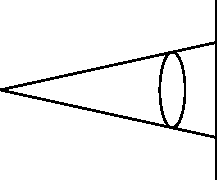
\includegraphics{epee_bocle/bocle_cone_proche}}
	\caption{Cônes de protections pour une bocle tenue loin et près.}
	\label{épée-bocle:fig:bocle-cone}
\end{figure}


\begin{exercice}[Défendre la main]

\D tend le bras droit devant lui et place sa main gauche près de sa main droite. 
\A essaie de toucher la main droite de \D qui ne peut se défendre qu'avec la main gauche.

Cet exercice travaille le fait de placer sa bocle du côté de l'épée adverse et de réagir vite pour l'intercepter.

Source : Arthur.

\end{exercice}


% fluidité
\begin{exercice}[Changements de garde]

Passer d'une garde à une autre en intercalant une frappe à chaque fois.
Chercher à être fluide.

\end{exercice}


\begin{exercice}[Couper la main]

\begin{enumerate}
	\item \A porte une attaque lente à \D, qui se défend simplement.
	\item Si une partie du corps de \A n'est pas protégée, alors \D amène son épée pour le mettre en évidence.
\end{enumerate}

\A peut enchaîner les frappes (en laissant le temps à \D de réagir pour mettre en évidence une éventuelle erreur).
Le but n'est pas d'aller vite mais de vérifier si la position est correcte.

Au début \D peut se concentrer uniquement sur la main d'arme de \A en faisant peu de mouvements, puis quand \A commence à avoir l'habitude \D peut chercher d'autres cibles et bouger légèrement.

\end{exercice}


\subsection{Gardes}


\begin{garde}[Crosse – \emph{Krucke}]
\index{krucke}
\index{garde!épée-bocle!krucke}

Dans la garde de la crosse (all. \emph{Krucke}, ang. \emph{crutch}), les mains sont placées face au visage, la pointe de l'épée vers le bas, la bocle couvrant la main d'arme.

\end{garde}

Cette garde est très hermétique et permet de dévier les estocs bas.


%%%%%%%%%%%%%%
\section{I.33}
%%%%%%%%%%%%%%


% type d'épée : Cinato : XVI, clubs allemands : XIV

% Royal Armouries, Tower Fechtbuch
Le traité MS I.33 (appelé aussi \emph{Walpurgis Fechtbuch} ou \emph{Liber de arte dimicatoria}) est le plus vieux manuel qui nous soit parvenu – il a été rédigé dans la décennie de 1320.
L'auteur serait un prêtre nommé Liutger.

La référence pour l'étude du I.33 est la traduction et le commentaire de Cinato et Suprenant~\cite{cinato:I33:2009}.
Kenner a écrit un manuel sur le sujet~\cite{kenner:I33:2014}.
Les images en couleur peuvent être trouvées sur le site de Wiktenauer~\cite{wiktenauer:I33}.


% TODO: custodia, contraria, liages supérieur/inférieur gauche/droit (inférieur = par en dessous)

\begin{definition}[Assiègement]
\index{assiègement}
\index{obsessio|see{assiègement}}
\index{contraria|see{assiègement}}

Un assiègement (lat. \emph{obsessio}~\cite{cinato:I33:2009}, \emph{contraria}~\cite{kenner:I33:2014}) est une position qui permet de briser une garde (lat. \emph{custodia}).

Il s'agit d'une position relativement hermétique et un assiègement adapté permet de se couvrir des attaques provenant de la garde adoptée par l'opposant.

\end{definition}

% liste des assiègement : krucke


\begin{definition}[Garde – \emph{Custodia}]
\index{garde!I.33}
\index{custodia|see{garde I.33}}

Une garde (lat. \emph{custodia}) est une position permettant de préparer une attaque.
Elle offre généralement une faible protection.

\end{definition}

% liste des gardes : 1 à 7

% TODO: déplacer en épée longue ?
\index{liage}
Il existe quatre liages possible : supérieur/inférieur et gauche/droite.
La personne qui lie est celle qui possède le centre et qui possède donc un avantage (plus ou moins important) sur l'autre.
Lorsque l'épée de celui qui lie est au-dessus on parle de liage supérieur, et de même si l'épée est en-dessous on parle de liage inférieur.
% cf Kenner

\begin{exercice}[Liages]

\begin{enumerate}
	\item \A fait un oberhau.
	\item \D vient prendre un liage.
	\item \A inverse le liage.
\end{enumerate}

L'oberhau est de hauteur variable pour encourager \D à varier les liages.
Le but n'est pas d'aller vite mais de sentir qui a le centre qui lie/est lié, de voir à quel point on est gêné et trouver le meilleur reliage.

\end{exercice}



%%%%%%%%%%%%%%%%%%%%
\section{Liegniczer}
%%%%%%%%%%%%%%%%%%%%


% TODO: add german words in techniques

Le traité de Liegniczer sur l'épée-bocle est très court et contient seulement six enchaînements.
On peut en trouver diverses transcriptions/traductions~\cite{ardamhe:liegniczer, farrell:liegnieczer, lindholm:ringeck_others:2006} ainsi que des interprétations~\cite{farrell:pedagogy_liegnieczer:2014, youtube:sala_armi:liegniczer, youtube:memag:liegniczer, lindholm:ringeck_others:2006, Myers:LiegniczerBuckler, knight:epee_bocle}.
Notre interprétation suit fortement~\cite{youtube:sala_armi:liegniczer, farrell:pedagogy_liegnieczer:2014}, ainsi que~\cite{youtube:memag:liegniczer}.

Le style développé par Liegniczer est très proche du système de Liechtenauer par le fait qu'il repose sur le concept de liage et de winden.
Il se rapproche aussi du I.33 par le fait que la bocle sert avant tout à couvrir la main d'arme, comme cela est indiqué dès le début de la première technique.
Keith Farrell a écrit un article sur la pédagogie de Liegniczer~\cite{farrell:pedagogy_liegnieczer:2014} afin de montrer que la structuration des six techniques présente bien un système cohérent et puissant.

Dans notre interprétation nous nous éloignons du livre de Lindholm, Svard and Clements~\cite{lindholm:ringeck_others:2006} qui ne nous semble pas correspondre tout à fait à l'esprit du système de Liegniczer : par exemple dans la technique 2, l'attaquant et les défenseurs séparent leurs deux mains.
% TODO: citer la page
De même l'interprétation de H.\ Knight~\cite[part I]{knight:epee_bocle} ne nous a pas convaincu, entre autres à cause des positions faibles qu'il adopte.

Dans chaque technique \A attaque tandis que \D est globalement passif : il semble que ce dernier ne soit pas initié à l'escrime et réagisse simplement avec des déflexions.
De même qu'en épée longue, \A va réagir d'une manière différente selon la réaction de \D, en apportant une réponse adaptée au mouvement de \D (ressenti).
% \emph{fühlen}
Ainsi qu'il a été expliqué plus haut, la bocle doit toujours protéger la main d'épée en se plaçant du même côté de l'épée de \D.
De même si \D ne prend pas soin de couvrir son bras alors \A doit frapper cette cible plus facile à atteindre.
Le seul moment où la bocle n'est pas utilisé pour couvrir la main est lorsque \A se trouve près de \D : dans ce cas la bocle est utilisée pour frapper et/ou contrôler les bras/mains de \D (entre autres lorsque l'on change d'axe ou que l'on vient chercher une cible basse).

L'idéal pour pratiquer ces techniques est de décomposer les techniques en séquences où \A doit réagir correctement selon ce que fait \D – d'abord en augmentant progressivement la longueur de l'enchaînement, puis en variant d'une fois à l'autre.


\begin{technique}[Liegniczer 1]
\label{épée-bocle:tech:liegniczer:1}

\A et \D démarrent dans la custodia 2 (épaule droite).

\begin{enumerate}
	\item \A lance un oberhau sur l'épaule droite de \D, en avançant la jambe droite.
	
	\item \D pare avec un oberhau, en avançant la jambe droite, et prend le liage.
	
	\item \alt{Si \D est faible, \A estoque.}
		Si \D est relativement fort au liage, \A exécute un winden en levant les mains en bœuf (en supination ou en pronation).
	
	\item \alt{Si \D ne réagit pas, \A estoque.}
		Si \D pousse la lame vers l'extérieur alors \A quitte le liage et vient frapper \D de l'autre côté en passant sous la lame (\emph{schnappen}),
		tout en frappant les mains de \D avec la bocle pour éloigner la menace.
\end{enumerate}

Au temps 3) le plus simple est de lever directement la main en supination ; cette position est relativement faible si l'on n'utilise pas le pouce en appui comme expliqué dans l'introduction de ce chapitre.
Le \emph{schnappen} au temps 4) sera d'autant plus efficace que \D écarte fort la lame – à l'extrême si \D écarte fort dès le temps 2) alors il n'y a pas de winden.

Pour illustrer nos explications générales, \A n'a pas besoin d'exécuter l'ensemble de la technique si \D fait une erreur.
Par exemple si \D est faible au temps 2) alors \A peut estoquer directement.

Au temps 2) les rôles sont symétriques et \D peut prendre l'initiative, auquel cas les rôles s'inversent.
De ce point de vue une autre manière d'interpréter l'enchaînement est que \D attaque \A qui prend le liage avec un oberhau, et ensuite enchaîne.

\end{technique}


\begin{figure}[htp]
	\centering
	\includegraphics{diagrammes/epee_bocle/liegniczer_1}
	\caption{Diagramme pour la technique 1 de Liegniczer.
	Nous n'indiquons pas le cas où \D ne réagit pas au premier oberhau.}
	\label{épée-bocle:fig:liegniczer:diagramme-1}
\end{figure}



\begin{technique}[Liegniczer 2]
\label{épée-bocle:tech:liegniczer:2}

\A démarre dans la custodia 5 (queue), \D dans la custodia 2 (épaule droite).

\begin{enumerate}
	\item \A lance un unterhau en avançant la jambe droite.
	
	\item \D prend le liage avec un oberhau en avançant la jambe droite.
	
	\item \alt{Si \D est faible, \A estoque.}
		Si \D est fort \A exécute un winden en levant les mains.
	
	\item \alt{Si \D ne réagit pas, \A estoque.}
		Si \D repousse la lame, \A exécute un duplieren tout en se décalant sur la gauche.
		La bocle permet de coincer l'épée de \D.
	
	\item \D se protège du coup et \A vient frapper les jambes du vrai tranchant (dans l'intérieur de \D).
\end{enumerate}

Il est possible d'inverser les temps 1) et 2) si l'on voit l'unterhau de \A comme un liage (inférieur).

\D se trouve naturellement jambe droite devant et il s'agit de la cible principale, alors que le traité indique que \A vise la jambe gauche : une interprétation est que \D peut toujours reculer la jambe droite, mais pas la gauche et si l'on vise cette dernière (ce qui est possible comme le coup est à l'intérieur) alors on est sûr de toucher quelque chose.

\end{technique}

% talhoffer : Myers:LiegniczerBuckler, knight:epee_bocle


\begin{technique}[Liegniczer 3]
\label{épée-bocle:tech:liegniczer:3}
% \index{coup!allemand!wechselhau}

\A et \D démarrent dans la custodia 2 (épaule droite).

\begin{enumerate}
	\item \A lance un oberhau en avançant la jambe droite.
	
	\item Quand \D se protège, \A laisse tomber la pointe de son épée sous celle de \D et la relève ensuite en battant fortement l'épée de \D avec le faux tranchant (coup changeant, wechselhau).
		\A se sert de l'élan pour frapper (du vrai tranchant) la tête de \D du côté droit en avançant la jambe gauche.
	% mouvement de hanches pour le balayage : permet d'éviter l'attaque ?
	
	\item \D se protège et \A exécute un winden en tournant la main en supination.
	
	\item \alt{Si \D ne fait rien, \A estoque.}
		\D dévie l'estoc et \A vient frapper la jambe droite du vrai tranchant.
		La bocle écarte les mains de \D.
\end{enumerate}

Au temps 2) le balayage est exécuté avec le faux tranchant car cela est plus rapide qu'avec le vrai, qui nécessiterait plusieurs rotations du poignet.
Il est aussi important de passer la bocle du côté droit du bras d'arme lors de la frappe, autant pour protéger le bras que pour laisser ouverte la ligne basse d'attaque.

La position en 3) n'est pas très forte : à notre avis l'idée est de surprendre en changeant la ligne d'attaque (technique~\ref{struct:tech:changement-ligne}).

Dans ce contexte la première attaque est une feinte.
Une autre interprétation est possible si \A commence dans la garde du fou : dans ce cas la déflexion en 2) est utilisée contre un oberhau de \D (pour une garde à gauche le balayage se fera naturellement avec le vrai tranchant).

\end{technique}


\begin{technique}[Liegniczer 4]
\label{épée-bocle:tech:liegniczer:4}
% \index{coup!allemand!mittelhau}

\A et \D démarrent dans la custodia 2 (épaule droite).

\begin{enumerate}
	\item \A lance un mittelhau (avec le vrai tranchant) à droite en avançant la jambe droite.
	
	\item \D se protège et \A frappe de l'autre côté avec un second mittelhau (vrai tranchant) en avançant la jambe gauche.
	
	\item \D se protège et \A lance un coup crânien (vrai tranchant) en avançant la jambe droite.
	
	\item \D se protège et \A fait glisser l'épée le long de la bocle de \D pour estoquer le ventre.
		\A garde sa bocle haute pour empêcher \D de baisser ses mains et pour protéger sa tête.
\end{enumerate}

L'idée de l'enchaînement est d'exécuter une série rapide de plusieurs coups qui vise à faire progressivement monter les défenses de \D afin d'attaquer bas à la fin.
Cela marche d'autant mieux si l'on a pu faire entrer \D dans un schéma, par exemple en lançant plusieurs mittelhau à la suite (par exemple avec un enchaînement droit-bas puis gauche-haut).

Les temps 1) et 2) constituent un double zwerchau, où la différence par rapport à l'épée longue est que la première frappe est faite avec le vrai tranchant.
Il est en effet un peu plus difficile de tourner la main sur la garde pour une épée une main puisque la main gauche n'est pas là pour stabiliser, et en gardant le pouce en appui sur les quillons il n'est pas possible de frapper avec le faux tranchant au temps 2) et 3).

Au temps 4) \A ne doit pas ramener son épée en arrière pour estoquer car il perdrait le centre (et du temps).

\end{technique}


\begin{technique}[Liegniczer 4 (variante)]
\label{épée-bocle:tech:liegniczer:4v}

\A et \D démarrent dans la custodia 2 (épaule droite).

\begin{enumerate}
	\item \A lance un mittelhau (avec le faux tranchant) à droite en avançant la jambe droite.
	
	\item \D se protège et \A frappe de l'autre côté avec un second mittelhau (vrai tranchant) en avançant la jambe gauche.
	
	\item \D se protège et \A lance un coup crânien (faux tranchant) en avançant la jambe droite.
	
	\item \D se protège et \A fait glisser l'épée le long de la bocle de \D pour estoquer le ventre.
		\A garde sa bocle haute pour empêcher \D de baisser ses mains et pour protéger sa tête.
\end{enumerate}

La différence avec la variante précédente est que deux des attaques – temps 1) et 3) – se font avec le faux tranchant, et ainsi la première attaque ressemble plus au zwerchau allemand que dans la première version.
Cet enchaînement est possible à condition que le pouce soit placé au niveau de la croix quillons/poignée, comme en épée longue, et que l'on conserve cette position tout le long.

Avec cette tenue la frappe en 3) avec le faux tranchant est très naturelle et plus rapide que si l'on devait ramener le vrai tranchant, et l'on dispose aussi d'un plus grand angle pour estoquer derrière la bocle (du fait de la position du poignet).

% Léo
\end{technique}


Une autre variante est proposée dans~\cite{youtube:sala_armi:liegniczer} : les mittelhaus sont respectivement portés à gauche et à droite.
Nous pensons que cet ordre est moins intéressant car il est quasiment certain qu le coup crânien tombera sur le bouclier ; mais cela reste une variation intéressante qui peut surprendre l'adversaire.


\begin{technique}[Liegniczer 5]
\label{épée-bocle:tech:liegniczer:5}

\A et \D démarrent dans la custodia 2 (épaule droite).

\begin{enumerate}
	\item \A lance un oberhau à droite en avançant la jambe droite, et tout en frappant tourne son poignet de 90° (sens direct) pour amener la pointe vers le bas, derrière le bouclier de \D (coup plongeant, sturtzhau).
	
	\item \alt{Si \D ne fait rien, \A estoque.}
		\D dévie l'estoc et \A fait contourne la bocle avec sa pointe pour venir estoquer le ventre : soit en descendant (rotation du poignet), soit en montant (rotation de l'épaule).
	
	\item \alt{Si \D ne fait rien, \A estoque.}
		\D dévie l'estoc (par exemple en passant en \emph{Krucke}) et \A exécute un winden en tournant la main en supination.
	
	\item \alt{Si \D ne fait rien, \A estoque.}
		\D dévie l'estoc vers sa droite et \A vient frapper la jambe droite du vrai tranchant.
		La bocle écarte les mains de \D.
\end{enumerate}

Au temps 1) l'oberhau est une feinte (mais si \D ne bouge pas alors il n'y a pas besoin de l'exécuter).
La fin de la technique est très similaire à celle de la séquence~3 (technique~\ref{épée-bocle:tech:liegniczer:3}).

Comme indiqué en 2) le contournement de la bocle peut se faire de deux manières.
Plusieurs interprétations favorisent un estoc descendant (en rapport avec la variante suivante), mais l'estoc montant semble favorisé dans la traduction de l'\textsc{Ardamhe}~\cite{ardamhe:liegniczer} : "monte la pointe par dessous".

Au temps 3) nous avons noté qu'une bonne défense pour \D est le \emph{Krucke}.
Elle est particulièrement adaptée si l'estoc est bas, mais elle ne correspond pas à une défense "naïve".
En Krucke \D peut sembler être protégé aux jambes : en fait lorsqu'il dévie l'estoc il commence à s'ouvrir, et la bocle permet d'écarter encore plus sa lame.

\end{technique}


\begin{technique}[Liegniczer 5 (variante)]
\label{épée-bocle:tech:liegniczer:5v}

\A et \D démarrent dans la custodia 2 (épaule droite).

\begin{enumerate}
	\item \A lance un oberhau à droite en avançant la jambe droite, et tout en frappant tourne son poignet de 90° (sens direct) pour amener la pointe vers le bas, derrière le bouclier de \D (coup plongeant, sturtzhau).
	
	\item Avant que \D ne dévie la pointe, \A contourne la bocle de \D grâce à une rotation du poignet, afin d'estoquer le côté droit de \D.
	
	\item \alt{Si \D ne fait rien, \A estoque.}
		\D dévie l'estoc et \A exécute un winden en tournant la main en supination.
	
	\item \alt{Si \D ne fait rien, \A estoque.}
		\D dévie l'estoc vers sa droite et \A vient frapper la jambe droite du vrai tranchant.
		La bocle écarte les mains de \D.
\end{enumerate}

Dans cette variante \A exécute deux feintes : d'abord en inversant la direction de la lame, puis en contournant la bocle.
Dans ce cas-là l'estoc au temps 2) est plus haut et \D devra utiliser une garde haute pour le dévier.

\end{technique}

\begin{figure}[htp]
	\centering
	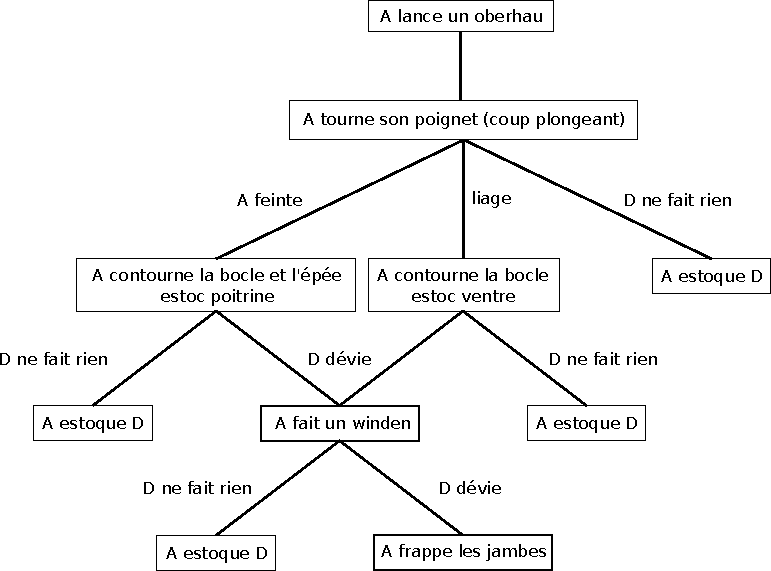
\includegraphics{diagrammes/epee_bocle/liegniczer_5}
	\caption{Diagramme pour la technique 5 de Liegniczer.}
	\label{épée-bocle:fig:liegniczer:diagramme-5}
\end{figure}


\begin{technique}[Liegniczer 6]

\A démarre dans une garde basse, \D dans la custodia 2 (épaule droite).

\begin{enumerate}
	\item \D lance un oberhau à droite en avançant la jambe droite.
	
	\item \A passe en demi-épée et fait une parade franche.
	
	\item \A lâche sa main droite et attrape la bocle de \D.
	
	\item \A arrache la bocle de \D.
	
	\item \A utilise la bocle pour frapper \D au visage.
\end{enumerate}

La meilleure manière pour retirer la bocle est de l'attraper par en-dessous (avec la paume tournée vers la droite) et de tourner dans le sens horaire~\footnotemark{}.
\footnotetext{Attention en pratiquant avec un partenaire : s'il a des gants épais ils peuvent rester coincés sous la poignée et la torsion peut être douloureuse.}

\A peut directement démarrer en demi-épée mais son intention peut alors être devinée plus facilement, sauf si la main est cachée par la bocle – par exemple grâce à la custodia 1 (sous le bras) ou si l'échange commence hors distance et \A adopte une position reposante.

À partir du moment où \A lâche sa poignée il doit la garder hors d'atteinte de \D.

\end{technique}


\chapter{Épée et bocle -- I.33}


% type d'épée : Cinato : XVI, clubs allemands : XIV

% Royal Armouries, Tower Fechtbuch
Le traité MS I.33 (appelé aussi \emph{Walpurgis Fechtbuch} ou \emph{Liber de arte dimicatoria}) est le plus vieux manuel qui nous soit parvenu – il a été rédigé dans la décennie de 1320.
L'auteur serait un prêtre nommé Liutger.

La référence pour l'étude du I.33 est la traduction et le commentaire de Cinato et Suprenant~\cite{cinato:I33:2009}.
Kenner a écrit un manuel sur le sujet~\cite{kenner:I33:2014}.
Les images en couleur peuvent être trouvées sur le site de Wiktenauer~\cite{wiktenauer:I33}.


% TODO: custodia, contraria, liages supérieur/inférieur gauche/droit (inférieur = par en dessous)

\begin{definition}[Assiègement]
\index{assiègement}
\index{obsessio|see{assiègement}}
\index{contraria|see{assiègement}}

Un assiègement (lat. \emph{obsessio}~\cite{cinato:I33:2009}, \emph{contraria}~\cite{kenner:I33:2014}) est une position qui permet de briser une garde (lat. \emph{custodia}).

Il s'agit d'une position relativement hermétique et un assiègement adapté permet de se couvrir des attaques provenant de la garde adoptée par l'opposant.
\end{definition}

% liste des assiègement : krucke


\begin{definition}[Garde – \emph{Custodia}]
\index{garde!I.33}
\index{custodia|see{garde I.33}}

Une garde (lat. \emph{custodia}) est une position permettant de préparer une attaque.
Elle offre généralement une faible protection.
\end{definition}

% liste des gardes : 1 à 7

% TODO: déplacer en épée longue ?
\index{liage}
Il existe quatre liages possible : supérieur/inférieur et gauche/droite.
La personne qui lie est celle qui possède le centre et qui possède donc un avantage (plus ou moins important) sur l'autre.
Lorsque l'épée de celui qui lie est au-dessus on parle de liage supérieur, et de même si l'épée est en-dessous on parle de liage inférieur.
% cf Kenner

Le liage doit être franc en écartant vraiment la lame adverse vers le bas.
Si on prend juste le centre sans bien éloigner la lame l'autre peut revenir facilement au moment où l'autre avance et attaquer gorge.

Rappelons aussi que les tranchants d'épées affûtées collent et il faut garder ceci à l'esprit en effectuant les mouvements (voir section~\ref{sec:armes-tranchantes:tranchant-collant}).


\begin{exercice}[Liages]

\begin{enumerate}
	\item \A fait un oberhau.
	\item \D vient prendre un liage.
	\item \A inverse le liage.
\end{enumerate}

L'oberhau est de hauteur variable pour encourager \D à varier les liages.
Le but n'est pas d'aller vite mais de sentir qui a le centre qui lie/est lié, de voir à quel point on est gêné et trouver le meilleur reliage.
\end{exercice}


\begin{exercice}
\A et \D sont en garde.
\D réunit ses deux mains devant lui (bras presque tendus) et \A vient placer son poing dedans.
\A essaie de repousser \D en poussant avec ses jambes.

Cet exercice doit être effectuer avec les deux mains.
Il prépare à donner des coups de bocles.

% Source : Thomas.
\end{exercice}


\begin{technique}

\A et \D démarrent au contact, pris en milieu de lame.

\begin{enumerate}
	\item \A prend le centre en liant l'épée vers la droite.
	\item \A donne un coup de bocle en avançant le pied gauche et vient trancher gorge.
\end{enumerate}

Test : en 1) \A ne repousse pas assez sur le côté, et alors en 2) \D revient au ventre et tranche gorge.

% \source{\cite{fuhrmann:dijon:I33_liage:2015}}
\end{technique}


\begin{exercice}[Liage et \emph{Krucke}]
\label{épée-bocle:I33:ex:krucke-liage}

\A et \D démarrent au contact, pris en milieu de lame.

\begin{enumerate}
	\item \A prend le centre en liant l'épée vers la droite.
	\item \D accepte le liage et monte son coude (\emph{Krucke}).
	\item \A continue d'avancer pour voir si \D tient bien.
\end{enumerate}

En 2) le mouvement est bon si \D relâche le poignet pour faire tomber l'épée, tout en montant le coude (comme en prime).
\D ne peut être ferme que s'il a placé son pouce sur le bord de la fusée, sous les quillons.
\D met sa bocle au dessus de sa main au cas où.

% \source{\cite{fuhrmann:dijon:I33_liage:2015}}
\end{exercice}


\begin{technique}

\A et \D démarrent au contact, pris en milieu de lame.

\begin{enumerate}
	\item \A prend le centre en liant l'épée vers la droite.
	\item \D accepte le liage (\emph{Krucke}).
	\item \A libère son tranchant et vient couper sur le plat de la lame de \D, en ramenant la main vers la gauche et en repoussant la lame.
	\item \A remonte les deux bras tendus dans l'ouverture pour frapper les mains de \D et estoquer au visage.
	\item Si \D réagit assez tôt, il abaisse les mains afin de bloquer la lame.
	\item \A fait un coup de bouclier et frappe au visage.
\end{enumerate}

En 3) \A casse son poignet. \A doit laisser sa pointe au centre.
Tout le long \A garde sa bocle bien sur sa main.
Au dernier temps si \A est bien placé il va ouvrir naturellement les bras de \D.

% \source{\cite{fuhrmann:dijon:I33_liage:2015}}
\end{technique}


\begin{technique}

\A et \D démarrent au contact, pris en milieu de lame.

\begin{enumerate}
	\item \A prend le centre en liant l'épée vers la droite.
	\item \D accepte le liage (\emph{Krucke}).
	\item \D ramène son bras gauche en arrière.
	\item \D arrête de reculer mais laisse son épée continuer derrière.
		Sous l'ouverture créée il donne un coup de bouclier, tout en faisant pivoter la lame (paume vers l'intérieur).
	\item \D laisse l'épée continuer son chemin et donne un coup de faux tranchant sur la tête de \A grâce à un arc vertical.
\end{enumerate}

Cette technique ne marche que si le contact du fer est assez haut.
Note que le fait que les lames sont collées permet à \D de tirer \A vers l'arrière alors même que lui n'avance plus.

% \source{\cite{fuhrmann:dijon:I33_liage:2015}}
\end{technique}


\begin{technique}

\A et \D démarrent au contact, pris en milieu de lame.

\begin{enumerate}
	\item \A prend le centre en liant l'épée vers la droite.
	\item \D accepte le liage (\emph{Krucke}).
	\item Tandis que \A continue d'avancer, \D décale son pied droit vers la droite et se retourner en entourant les bras de \A pour les bloquer.
\end{enumerate}

% Marche mieux que la technique précédente quand le contact est plus bas (?).

% \source{\cite{fuhrmann:dijon:I33_liage:2015}}
\end{technique}


\begin{technique}

\A et \D démarrent au contact, pris en milieu de lame.

\begin{enumerate}
	\item \A prend le centre en liant l'épée vers la droite.
	\item \D accepte le liage (\emph{Krucke}).
	\item \D tourne les hanches et retourne le bras pour frapper sur la lame de \A.
\end{enumerate}

% Marche mieux que la technique avant la précédente quand le contact est plus bas (?).
Si cela ne marche pas, remonter pour trancher les bras.

% \source{\cite{fuhrmann:dijon:I33_liage:2015}}
\end{technique}

\chapter{Épée et bocle -- Liegniczer}


% TODO: add german words in techniques

Le traité de Liegniczer sur l'épée-bocle est très court et contient seulement six enchaînements.
On peut en trouver diverses transcriptions/traductions~\cite{ardamhe:liegniczer, farrell:liegnieczer, lindholm:ringeck_others:2006} ainsi que des interprétations~\cite{farrell:pedagogy_liegnieczer:2014, youtube:sala_armi:liegniczer, youtube:memag:liegniczer, lindholm:ringeck_others:2006, Myers:LiegniczerBuckler, knight:epee_bocle}.
Notre interprétation suit fortement~\cite{youtube:sala_armi:liegniczer, farrell:pedagogy_liegnieczer:2014}, ainsi que~\cite{youtube:memag:liegniczer}.

Le style développé par Liegniczer est très proche du système de Liechtenauer par le fait qu'il repose sur le concept de liage et de winden.
Il se rapproche aussi du I.33 par le fait que la bocle sert avant tout à couvrir la main d'arme, comme cela est indiqué dès le début de la première technique.
Keith Farrell a écrit un article sur la pédagogie de Liegniczer~\cite{farrell:pedagogy_liegnieczer:2014} afin de montrer que la structuration des six techniques présente bien un système cohérent et puissant.

Dans notre interprétation nous nous éloignons du livre de Lindholm, Svard and Clements~\cite{lindholm:ringeck_others:2006} qui ne nous semble pas correspondre tout à fait à l'esprit du système de Liegniczer : par exemple dans la technique 2, l'attaquant et les défenseurs séparent leurs deux mains.
% TODO: citer la page
De même l'interprétation de H.\ Knight~\cite[part I]{knight:epee_bocle} ne nous a pas convaincu, entre autres à cause des positions faibles qu'il adopte.

Dans chaque technique \A attaque tandis que \D est globalement passif : il semble que ce dernier ne soit pas initié à l'escrime et réagisse simplement avec des déflexions.
De même qu'en épée longue, \A va réagir d'une manière différente selon la réaction de \D, en apportant une réponse adaptée au mouvement de \D (ressenti).
% \emph{fühlen}
Ainsi qu'il a été expliqué plus haut, la bocle doit toujours protéger la main d'épée en se plaçant du même côté de l'épée de \D.
De même si \D ne prend pas soin de couvrir son bras alors \A doit frapper cette cible plus facile à atteindre.
Le seul moment où la bocle n'est pas utilisé pour couvrir la main est lorsque \A se trouve près de \D : dans ce cas la bocle est utilisée pour frapper et/ou contrôler les bras/mains de \D (entre autres lorsque l'on change d'axe ou que l'on vient chercher une cible basse).

L'idéal pour pratiquer ces techniques est de décomposer les techniques en séquences où \A doit réagir correctement selon ce que fait \D – d'abord en augmentant progressivement la longueur de l'enchaînement, puis en variant d'une fois à l'autre.


\begin{technique}[Liegniczer 1]
\label{épée-bocle:tech:liegniczer:1}

\A et \D démarrent dans la custodia 2 (épaule droite).

\begin{enumerate}
	\item \A lance un oberhau sur l'épaule droite de \D, en avançant la jambe droite.
	
	\item \D pare avec un oberhau, en avançant la jambe droite, et prend le liage.
	
	\item \alt{Si \D est faible, \A estoque.}
		Si \D est relativement fort au liage, \A exécute un winden en levant les mains en bœuf (en supination ou en pronation).
	
	\item \alt{Si \D ne réagit pas, \A estoque.}
		Si \D pousse la lame vers l'extérieur alors \A quitte le liage et vient frapper \D de l'autre côté en passant sous la lame (\emph{schnappen}),
		tout en frappant les mains de \D avec la bocle pour éloigner la menace.
\end{enumerate}

Au temps 3) le plus simple est de lever directement la main en supination ; cette position est relativement faible si l'on n'utilise pas le pouce en appui comme expliqué dans l'introduction de ce chapitre.
Le \emph{schnappen} au temps 4) sera d'autant plus efficace que \D écarte fort la lame – à l'extrême si \D écarte fort dès le temps 2) alors il n'y a pas de winden.

Pour illustrer nos explications générales, \A n'a pas besoin d'exécuter l'ensemble de la technique si \D fait une erreur.
Par exemple si \D est faible au temps 2) alors \A peut estoquer directement.

Au temps 2) les rôles sont symétriques et \D peut prendre l'initiative, auquel cas les rôles s'inversent.
De ce point de vue une autre manière d'interpréter l'enchaînement est que \D attaque \A qui prend le liage avec un oberhau, et ensuite enchaîne.

\end{technique}


\begin{figure}[htp]
	\centering
	\includegraphics{diagrammes/epee_bocle/liegniczer_1}
	\caption{Diagramme pour la technique 1 de Liegniczer.
	Nous n'indiquons pas le cas où \D ne réagit pas au premier oberhau.}
	\label{épée-bocle:fig:liegniczer:diagramme-1}
\end{figure}



\begin{technique}[Liegniczer 2]
\label{épée-bocle:tech:liegniczer:2}

\A démarre dans la custodia 5 (queue), \D dans la custodia 2 (épaule droite).

\begin{enumerate}
	\item \A lance un unterhau en avançant la jambe droite.
	
	\item \D prend le liage avec un oberhau en avançant la jambe droite.
	
	\item \alt{Si \D est faible, \A estoque.}
		Si \D est fort \A exécute un winden en levant les mains.
	
	\item \alt{Si \D ne réagit pas, \A estoque.}
		Si \D repousse la lame, \A exécute un duplieren tout en se décalant sur la gauche.
		La bocle permet de coincer l'épée de \D.
	
	\item \D se protège du coup et \A vient frapper les jambes du vrai tranchant (dans l'intérieur de \D).
\end{enumerate}

Il est possible d'inverser les temps 1) et 2) si l'on voit l'unterhau de \A comme un liage (inférieur).

\D se trouve naturellement jambe droite devant et il s'agit de la cible principale, alors que le traité indique que \A vise la jambe gauche : une interprétation est que \D peut toujours reculer la jambe droite, mais pas la gauche et si l'on vise cette dernière (ce qui est possible comme le coup est à l'intérieur) alors on est sûr de toucher quelque chose.

\end{technique}

% talhoffer : Myers:LiegniczerBuckler, knight:epee_bocle


\begin{technique}[Liegniczer 3]
\label{épée-bocle:tech:liegniczer:3}
% \index{coup!allemand!wechselhau}

\A et \D démarrent dans la custodia 2 (épaule droite).

\begin{enumerate}
	\item \A lance un oberhau en avançant la jambe droite.
	
	\item Quand \D se protège, \A laisse tomber la pointe de son épée sous celle de \D et la relève ensuite en battant fortement l'épée de \D avec le faux tranchant (coup changeant, wechselhau).
		\A se sert de l'élan pour frapper (du vrai tranchant) la tête de \D du côté droit en avançant la jambe gauche.
	% mouvement de hanches pour le balayage : permet d'éviter l'attaque ?
	
	\item \D se protège et \A exécute un winden en tournant la main en supination.
	
	\item \alt{Si \D ne fait rien, \A estoque.}
		\D dévie l'estoc et \A vient frapper la jambe droite du vrai tranchant.
		La bocle écarte les mains de \D.
\end{enumerate}

Au temps 2) le balayage est exécuté avec le faux tranchant car cela est plus rapide qu'avec le vrai, qui nécessiterait plusieurs rotations du poignet.
Il est aussi important de passer la bocle du côté droit du bras d'arme lors de la frappe, autant pour protéger le bras que pour laisser ouverte la ligne basse d'attaque.

La position en 3) n'est pas très forte : à notre avis l'idée est de surprendre en changeant la ligne d'attaque (technique~\ref{struct:tech:changement-ligne}).

Dans ce contexte la première attaque est une feinte.
Une autre interprétation est possible si \A commence dans la garde du fou : dans ce cas la déflexion en 2) est utilisée contre un oberhau de \D (pour une garde à gauche le balayage se fera naturellement avec le vrai tranchant).

\end{technique}


\begin{technique}[Liegniczer 4]
\label{épée-bocle:tech:liegniczer:4}
% \index{coup!allemand!mittelhau}

\A et \D démarrent dans la custodia 2 (épaule droite).

\begin{enumerate}
	\item \A lance un mittelhau (avec le vrai tranchant) à droite en avançant la jambe droite.
	
	\item \D se protège et \A frappe de l'autre côté avec un second mittelhau (vrai tranchant) en avançant la jambe gauche.
	
	\item \D se protège et \A lance un coup crânien (vrai tranchant) en avançant la jambe droite.
	
	\item \D se protège et \A fait glisser l'épée le long de la bocle de \D pour estoquer le ventre.
		\A garde sa bocle haute pour empêcher \D de baisser ses mains et pour protéger sa tête.
\end{enumerate}

L'idée de l'enchaînement est d'exécuter une série rapide de plusieurs coups qui vise à faire progressivement monter les défenses de \D afin d'attaquer bas à la fin.
Cela marche d'autant mieux si l'on a pu faire entrer \D dans un schéma, par exemple en lançant plusieurs mittelhau à la suite (par exemple avec un enchaînement droit-bas puis gauche-haut).

Les temps 1) et 2) constituent un double zwerchau, où la différence par rapport à l'épée longue est que la première frappe est faite avec le vrai tranchant.
Il est en effet un peu plus difficile de tourner la main sur la garde pour une épée une main puisque la main gauche n'est pas là pour stabiliser, et en gardant le pouce en appui sur les quillons il n'est pas possible de frapper avec le faux tranchant au temps 2) et 3).

Au temps 4) \A ne doit pas ramener son épée en arrière pour estoquer car il perdrait le centre (et du temps).

\end{technique}


\begin{technique}[Liegniczer 4 (variante)]
\label{épée-bocle:tech:liegniczer:4v}

\A et \D démarrent dans la custodia 2 (épaule droite).

\begin{enumerate}
	\item \A lance un mittelhau (avec le faux tranchant) à droite en avançant la jambe droite.
	
	\item \D se protège et \A frappe de l'autre côté avec un second mittelhau (vrai tranchant) en avançant la jambe gauche.
	
	\item \D se protège et \A lance un coup crânien (faux tranchant) en avançant la jambe droite.
	
	\item \D se protège et \A fait glisser l'épée le long de la bocle de \D pour estoquer le ventre.
		\A garde sa bocle haute pour empêcher \D de baisser ses mains et pour protéger sa tête.
\end{enumerate}

La différence avec la variante précédente est que deux des attaques – temps 1) et 3) – se font avec le faux tranchant, et ainsi la première attaque ressemble plus au zwerchau allemand que dans la première version.
Cet enchaînement est possible à condition que le pouce soit placé au niveau de la croix quillons/poignée, comme en épée longue, et que l'on conserve cette position tout le long.

Avec cette tenue la frappe en 3) avec le faux tranchant est très naturelle et plus rapide que si l'on devait ramener le vrai tranchant, et l'on dispose aussi d'un plus grand angle pour estoquer derrière la bocle (du fait de la position du poignet).

% Léo
\end{technique}


Une autre variante est proposée dans~\cite{youtube:sala_armi:liegniczer} : les mittelhaus sont respectivement portés à gauche et à droite.
Nous pensons que cet ordre est moins intéressant car il est quasiment certain qu le coup crânien tombera sur le bouclier ; mais cela reste une variation intéressante qui peut surprendre l'adversaire.


\begin{technique}[Liegniczer 5]
\label{épée-bocle:tech:liegniczer:5}

\A et \D démarrent dans la custodia 2 (épaule droite).

\begin{enumerate}
	\item \A lance un oberhau à droite en avançant la jambe droite, et tout en frappant tourne son poignet de 90° (sens direct) pour amener la pointe vers le bas, derrière le bouclier de \D (coup plongeant, sturtzhau).
	
	\item \alt{Si \D ne fait rien, \A estoque.}
		\D dévie l'estoc et \A fait contourne la bocle avec sa pointe pour venir estoquer le ventre : soit en descendant (rotation du poignet), soit en montant (rotation de l'épaule).
	
	\item \alt{Si \D ne fait rien, \A estoque.}
		\D dévie l'estoc (par exemple en passant en \emph{Krucke}) et \A exécute un winden en tournant la main en supination.
	
	\item \alt{Si \D ne fait rien, \A estoque.}
		\D dévie l'estoc vers sa droite et \A vient frapper la jambe droite du vrai tranchant.
		La bocle écarte les mains de \D.
\end{enumerate}

Au temps 1) l'oberhau est une feinte (mais si \D ne bouge pas alors il n'y a pas besoin de l'exécuter).
La fin de la technique est très similaire à celle de la séquence~3 (technique~\ref{épée-bocle:tech:liegniczer:3}).

Comme indiqué en 2) le contournement de la bocle peut se faire de deux manières.
Plusieurs interprétations favorisent un estoc descendant (en rapport avec la variante suivante), mais l'estoc montant semble favorisé dans la traduction de l'\textsc{Ardamhe}~\cite{ardamhe:liegniczer} : "monte la pointe par dessous".

Au temps 3) nous avons noté qu'une bonne défense pour \D est le \emph{Krucke}.
Elle est particulièrement adaptée si l'estoc est bas, mais elle ne correspond pas à une défense "naïve".
En Krucke \D peut sembler être protégé aux jambes : en fait lorsqu'il dévie l'estoc il commence à s'ouvrir, et la bocle permet d'écarter encore plus sa lame.
% mais en essayant au début on a vu que ça pouvait être compliqué de réussir, d'où l'idée de garder la main haute

\end{technique}


\begin{technique}[Liegniczer 5 (variante)]
\label{épée-bocle:tech:liegniczer:5v}

\A et \D démarrent dans la custodia 2 (épaule droite).

\begin{enumerate}
	\item \A lance un oberhau à droite en avançant la jambe droite, et tout en frappant tourne son poignet de 90° (sens direct) pour amener la pointe vers le bas, derrière le bouclier de \D (coup plongeant, sturtzhau).
	
	\item Avant que \D ne dévie la pointe, \A contourne la bocle de \D grâce à une rotation du poignet, afin d'estoquer le côté droit de \D.
	
	\item \alt{Si \D ne fait rien, \A estoque.}
		\D dévie l'estoc et \A exécute un winden en tournant la main en supination.
	
	\item \alt{Si \D ne fait rien, \A estoque.}
		\D dévie l'estoc vers sa droite et \A vient frapper la jambe droite du vrai tranchant.
		La bocle écarte les mains de \D.
\end{enumerate}

Dans cette variante \A exécute deux feintes : d'abord en inversant la direction de la lame, puis en contournant la bocle.
Dans ce cas-là l'estoc au temps 2) est plus haut et \D devra utiliser une garde haute pour le dévier.

\end{technique}

\begin{figure}[htp]
	\centering
	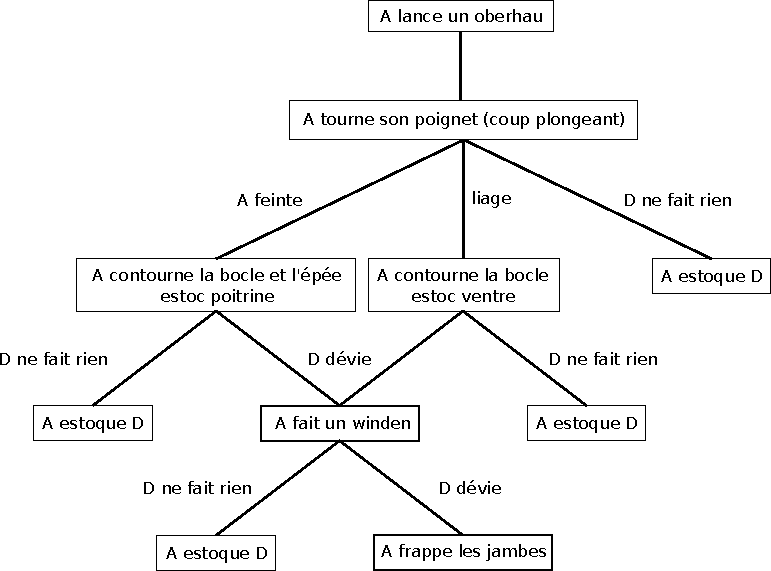
\includegraphics{diagrammes/epee_bocle/liegniczer_5}
	\caption{Diagramme pour la technique 5 de Liegniczer.}
	\label{épée-bocle:fig:liegniczer:diagramme-5}
\end{figure}


\begin{technique}[Liegniczer 6]

\A démarre dans une garde basse, \D dans la custodia 2 (épaule droite).

\begin{enumerate}
	\item \D lance un oberhau à droite en avançant la jambe droite.
	
	\item \A passe en demi-épée et fait une parade franche.
	
	\item \A lâche sa main droite et attrape la bocle de \D.
	
	\item \A arrache la bocle de \D.
	
	\item \A utilise la bocle pour frapper \D au visage.
\end{enumerate}

La meilleure manière pour retirer la bocle est de l'attraper par en-dessous (avec la paume tournée vers la droite) et de tourner dans le sens horaire~\footnotemark{}.
\footnotetext{Attention en pratiquant avec un partenaire : s'il a des gants épais ils peuvent rester coincés sous la poignée et la torsion peut être douloureuse.}

\A peut directement démarrer en demi-épée mais son intention peut alors être devinée plus facilement, sauf si la main est cachée par la bocle – par exemple grâce à la custodia 1 (sous le bras) ou si l'échange commence hors distance et \A adopte une position reposante.

À partir du moment où \A lâche sa poignée il doit la garder hors d'atteinte de \D.

\end{technique}


\chapter{Épée et bouclier viking}


Le bouclier viking est circulaire et plat.
Plusieurs armes peuvent être utilisées en combinaison avec le bouclier : dans ce chapitre nous discuterons de l'épée.
Les cibles possibles sont : la jambe sous le bouclier (derrière le genou) et le côté opposé.
Il faut utiliser le manque de visibilité pour attaquer.
De plus il est important de toujours protéger le bras qui attaque.
Si l'adversaire ne protège pas son bras il suffit d'attaquer cette cible pour mettre fin au combat.

Il faut noter que le bouclier est une arme par lui-même : une attaque fréquente consiste à donner un coup du poing gauche, ce qui revient à donner un coup horizontal du bouclier.

\noindent
Quelques idées pour attaquer :
\begin{itemize}
	\item pied gauche en avant, attaque droit devant (avec ou sans changement de pied) ;
	\item à partir de l'attaque précédente ou en garde, tourner le poignet gauche vers la droite, ce qui inverse verticalement le bouclier, et passer le bouclier par dessus le bras droit.
	En même temps, le poignet droit pivote vers la gauche – le tranchant se tourne vers le haut – en déplaçant le bras vers la gauche, et il ne reste plus qu'à attaquer ;
	\item l'attaque précédente peut se faire sans tourner l'épée, ce qui mène à une attaque de bas en haut ;
	\item elle peut aussi se faire en sens inverse pour revenir dans la position de départ.
\end{itemize}

Si \A attaque \D à la tête (peu importe le côté) alors \D a juste à lever le bouclier pour être protégé.
L'idée générale pour l'attaquant est de faire semblant d'attaquer en haut et d'essayer ensuite de frapper un autre endroit en tirant parti du fait que le défenseur ne peut pas le voir derrière son bouclier.
Plusieurs options sont possibles :
\begin{itemize}
	\item dévier légèrement l'attaque pour la faire passer à côté du bouclier et trancher la jambe ;
	\item contourner le bouclier par en dessous et remonter vers le ventre (en passant sous la cotte de maille) ;
	\item l'attaque précédente peut se faire aussi dans le dos ;
	\item enfin en remontant plus haut on peut viser la gorge ;
	\item et enfin, un peu moins convaincant, dévier pour amener l'épée derrière le genou ennemi et trancher les tendons.
\end{itemize}
En exercice le défenseur peut dire s'il a réussi à voir l'attaque venir.


\begin{technique}

\begin{enumerate}
	\item \A attaque.
	
	\item \D pare avec son bouclier.
	
	\item En avançant le pied gauche, \A percute \D (entre le coude et l'épaule gauche) avec son bouclier pour briser/engourdir le bras.
	
	\item \A attaque la jambe gauche avec son épée.
\end{enumerate}
\end{technique}


\begin{technique}

\begin{enumerate}
	\item \A feinte en attaquant \D.
	
	\item Si \D pare assez haut avec son bouclier, alors \A frappe l'épaule de son ennemi avec son bouclier en réarmant.
	
	\item \A abat son épée sur le bras (ce qui permet au moins de trancher la guige).
\end{enumerate}
\end{technique}


Si \D garde son bouclier bien devant soi (par exemple après une des deux techniques précédentes) alors \A peut donner un coup de son bouclier sur le côté gauche (vu de face) afin de le faire pivoter, ce qui découvre le flanc de \D.
\A peut alors porter un estoc.

Une autre technique consiste à faire en sorte de forcer l'adversaire à ouvrir sa garde, en attaquant d'abord sur sa droite (ce qui lui fait ramener son épée et son bouclier de ce côté), puis rapidement sur sa gauche (lui faisant déplacer son bouclier), et pendant qu'il est ouvert on peut donner un coup de bouclier sur l'épaule puis couper un bras.

\begin{technique}

\A et \D commencent jambe gauche en avant.

\begin{enumerate}
	\item \A attaque la jambe sous le bouclier (gauche).
	
	\item \D avance le bras gauche pour couvrir (mais sans le descendre, car le fait d'avancer suffit pour protéger).
	
	\item \D frappe avec son épée le dos de l'avant-bras de \A par au-dessus.
\end{enumerate}
\end{technique}


% \input{chapters/ecu}


\part{Armes d'hast}

\chapter{Bâton long}


Le bâton long est un simple bâton dont la taille est approximativement de deux mètres.
Il faut se rappeler lors de la pratique amicale que le bâton est une arme en tant que telle : nous ne travaillons pas avec un simulateur.

Une main tient l'extrémité et l'autre est placée quelques paumes plus loin : l'écartement entre les mains est approximativement égal à la largeur des épaules ou un peu plus grand.
Plus l'écartement est grand plus la main avant sera exposée aux frappes de l'adversaire, mais il s'agit aussi d'une prise plus facile au début.
% Katori : largeur des épaules
Il existe deux manières de tenir le bâton :
\begin{itemize}
	\item prise lance : la main avant est en supination, les deux pouces sont tournés vers l'avant ;
	\item prise bâton : la main avant est en pronation, les deux pouces sont tournés l'un vers l'autre.
\end{itemize}
Nous nous occuperons principalement de la seconde prise.
Par main avant nous désignerons toujours la main qui se trouve le plus en avant sur le bâton, pas nécessairement la main qui se trouve la plus proche de l'adversaire.

Les attaques au bâton sont principalement des coups de taille armés sur le côté, des coups de taille circulaire et des estocs.


\begin{coup}[Frappe diagonale descendante au bâton]
\index{coup!bâton long}

Le coup est armé en plaçant la main avant au niveau de l'épaule et la main arrière au niveau du plexus, le bâton est dirigé vers le haut.
Le pied en arrière est le même que la main à l'avant du bâton.
La frappe se fait en abattant le bâton selon une direction diagonale grâce à un mouvement de hanche.
\end{coup}


\begin{coup}[Frappe diagonale ascendante au bâton]

Le coup est armé en plaçant la main avant au niveau de la hanche droite et la main arrière au niveau de la hanche gauche, le bâton est horizontal et dirigé vers l'arrière.
Le pied en arrière est le même que la main à l'avant du bâton.
La frappe se fait remontant les deux mains au niveau de la tête.
\end{coup}


% TODO: améliorer
\begin{coup}[Frappe droite descendante au bâton]

Le coup est armé en plaçant la main avant au niveau de l'épaule et la main arrière au niveau du plexus, le bâton est dirigé vers le haut.
Le pied en arrière est le même que la main à l'avant du bâton.
La frappe se fait en abattant le bâton droit devant soi (les mains se retrouvent alignées au centre de la personne).
\end{coup}


La partie qui heurte l'adversaire doit être l'extrémité du bâton car il s'agit de la partie qui possède le plus d'énergie cinétique.
Les cibles au bâton long sont les suivantes : les tempes, la nuque, les omoplates, les coudes, les poignets, les genoux et les chevilles (en résumé la plupart des articulations).
\index{cible!bâton long}
% TODO: schéma

L'idée du bâton long est d'armer très rapidement après avoir frappé : ainsi l'adversaire se trouve sous la menace d'une nouvelle frappe et ne peut pas prendre l'initiative (surtout s'il a une arme plus courte).
La manière d'armer demande de l'entraînement pour être réalisé rapidement et efficacement, mais elle est assez naturelle : il s'agit de tirer le bâton avec la main arrière et de le laisser glisser entre les doigts légèrement desserrés.
Ce mouvement est très rapide et permet de soustraire notre bâton à l'adversaire.
En effet plus notre bâton reste longtemps près de l'adversaire plus celui-ci peut en prendre le contrôle (et ce même s'il est bien verrouillé -- voire plus bas).
Pour cette raison après une attaque il est plus prudent soit d'enchaîner directement avec une autre attaque, soit de réarmer en arrière.
Pendant le bref instant où le bâton se trouve en avant on doit se retrouver dans une des gardes décrites plus bas.

% Les estocs sont très naturels au bâton et visent principalement le ventre, le torse et la tête.


\index{verrouillage}
Un concept important au bâton (et aux armes d'hast en générale) est celui de verrouillage : la main (ou l'avant-bras) arrière doit toujours être bloquée contre une partie du corps.
Cela permet de s'assurer que l'adversaire ne peut pas éjecter facilement le bâton (par exemple avec un enroulé).
Pour une garde basse le verrouillage se fait contre la hanche arrière tandis que pour une garde haute il se fait à la tête.


\begin{garde}[Garde basse]
\index{garde!bâton long}

La main arrière est calée contre la hanche, et le coude avant près du corps.
Le bâton est étendu devant soi.
\end{garde}


\begin{garde}[Garde haute]

La main arrière est au-dessus de la tête, l'autre devant, avec les doigts dépliés derrière le bâton (pour éviter les coups dessus).
\end{garde}


En garde haute les attaques hautes sont bloquées avec la partie comprise entre les deux mains.

En position de garde il est important que le bâton de l'adversaire ne soit pas derrière le nôtre (c'est-à-dire du côté où se trouvent nos bras) car il lui est alors facile de rentrer en lutte ou d'attaquer les bras (et la partie arrière du bâton n'est plus utilisable).
Ainsi selon les gardes respectives, soit aucun n'est désavantagé, soit un l'est, soit les deux le sont.
On définira la garde "normale" comme celle où aucun n'est avantagé (par exemple les deux ont le pied gauche en avant et chacun est protégé par son bâton).


\begin{exercice}

\obj{S'entrainer à enchainer des coups.}

\begin{enumerate}
	\item À partir de la garde tirer sur le bâton avec la main arrière pour le ramener derrière.
	
	\item Abaisser les bras (en "fouettant") pour porter l'attaque.
	
	\item Se retrouver dans la garde opposer.
\end{enumerate}

De même en faisant une attaque montante on se retrouve en garde haute.
\end{exercice}


\begin{exercice}

Vérifier qu'en garde haute il suffit de peu d'efforts pour bloquer les attaques simples.
\end{exercice}

\chapter{Bâton long -- prise milieu}


Les deux mains sont placées de manière symétrique par rapport au centre.
L'avantage de cette prise est de permettre une plus grande mobilité lors des parades et des frappes.
Par exemple il est possible de parer d'un côté et d'attaquer immédiatement de l'autre.

Les cibles sont les mêmes que pour la tenue longue.
De même il existe trois gardes, dont deux sont identiques à la prise longue.


\begin{garde}[Garde de la barrière]
\index{garde!bâton long}

Le bâton est tenu verticalement devant soi, (presque) posé sur le sol, les bras sont tendus.
\end{garde}


\begin{technique}

\begin{enumerate}
	\item Depuis la garde, \A ramène un peu ses bras vers lui pour faire passer son arme au-dessus de celle de l'adversaire afin d'attaquer le poignet, en faisant un appel de pied.
	
	\item \D, d'un même mouvement, ramène la partie avant de son bâton vers la gauche pour écarter le bâton adversaire et fait tourner son bâton en changeant de pied pour attaquer le coup avec la partie arrière.
	
	\item \A bloque verticalement en avançant, la partie arrière du bâton se retrouvant en haut.
	
	\item \A abaisse le bâton pour frapper le coude.
	
	\item \A frappe de l'autre côté (verticalement, donc le bâton reste du même côté et se retrouve sous le bras).
	
	\item \A frappe horizontalement la nuque en faisant un cercle horaire.
	
	\item \A frappe le cou verticalement.
\end{enumerate}

Pour parer le premier coup \D peut baisser son bâton pour le faire passer sous celui de l'ennemi afin de le ramener devant.
Lorsque \A bloque il peut le faire en reculant, auquel cas la parade la plus "sûre" se fait avec la partie arrière du bâton en haut.

% TODO: technique séparée
Une variante consiste à parer en reculant sans retourner le bâton, ce qui permet de se retrouver dans la bonne position pour insérer son bâton entre le bras et le bâton de l'adversaire, ce qui permet de le contrôler (torsion, désarmement, etc.).
\end{technique}


% à partir de la garde verticale, quand on se retrouve à l'intérieur de la garde adverse (i.e. entre lui et son bâton), il faut alors avancer rapidement, ce qui permet de casser le poignet et d'entrer en lutte

% une parade consiste à reculer en lâchant le bâton de la main avant, puis le faire tourner pour le saisir comme une lance puis à l'abaisser


\chapter{Lance}


\section{Généralités}

% Romain
La lance est une arme qui doit être très mobile et offensive.
Pour cette raison il n'est souvent pas intéressant de verrouiller la main (contre la hanche ou a tête) afin de pouvoir changer rapidement de direction d'attaque.
De plus en bougeant souvent la lance l'adversaire aura peu l'occasion de la dégager via un enroulé ; de même il sera beaucoup plus simple de ramener la pointe dans le centre si l'adversaire porte un coup puissant contre le manche.
Au contraire le verrouillage pourra être utile dans les formations serrées (par exemple de piquiers~\footnotemark).
\footnotetext{Ceux-ci verrouillaient le manche en le posant sur leur ceinture, qui était portée plus haut que nous.}
% ~\footnote{Une poussée par des lanciers peut désorganiser un mur de boucliers.}

La lance peut aussi être tenue de deux manières, comme le bâton long : toutefois on observera le plus souvent la tenue où les deux pouces sont tournés du même côté.
Cette tenue facilite aussi le fait de coulisser la lance dans la main avant afin de porter un estoc tout en gagnant de l'allonge.

% TODO: gardes

\begin{coup}[Attaque basse]
En garde basse, la main avant est la même que celle du pied avant.
Avancer le pied avant et faire coulisser le manche dans la main avant pour estoquer.
\end{coup}


\begin{coup}[Attaque haute]
En garde haute, la main avant est la même que celle du pied avant.
Avancer le pied avant et faire coulisser le manche dans la main avant pour estoquer.
La lance a une direction descendante.
\end{coup}

Cette seconde attaque est utile pour piquer derrière un bouclier, à la tête.

\begin{technique}[Retour en garde haute]
Après une attaque basse, monter la main arrière et descendre sur les appuis.
La main avant se place sous la hampe pour protéger les doigts (si prise bâton, placer le poing).

Une amélioration consiste à placer l'avant bras.
\end{technique}

Dans la garde précédente où l'avant-bras est placé contre le manche, avec une hallebarde on est alors très bien placé pour frapper avec le tranchant par en haut.

\begin{technique}[Retour en garde basse]
Après une attaque haute, faire un tour avec la pointe en tournant la main gauche (arrière) dans le sens antihoraire (comme un rameur), et revenir en garde basse en ramenant la main en bas.
Le tour permet de reprendre le centre, sinon la lance peut se retrouver à l'extérieur.
Et si l'autre n'est pas prudent il est possible de le planter direct.
\end{technique}


\section{Lance contre épée courte}


\begin{exercice}

\A porte l'épée.

\begin{enumerate}
	\item \A part en garde de quarte (pied droit en avant) ou de tierce (gauche en avant) et change de garde en faisant passer son épée sous la lance.
\end{enumerate}

Le centre de gravité de l'épée reste fixe, et la lame doit rester tout le temps en contact avec la hampe de la lance pour garder le contrôle.

Le lancier peut aussi avancer pour compliquer l'exercice.
\end{exercice}


\begin{technique}

\D est armé de la lance et démarre pied gauche devant.
\A démarre pied droit devant.

\begin{enumerate}
	\item \A vient bloquer en tierce la lame.
	
	\item \A passe rapidement sous son bras droit en passant le pied gauche devant, pour ensuite frapper \D.
\end{enumerate}

Le temps 1) est une feinte qui laisse croire au lancier qu'il va pouvoir l'embrocher.
\end{technique}


\begin{technique}

\D est armé de la lance.

\begin{enumerate}
	\item \D recule en donnant des coups d'estoc.
	
	\item \A fait semblant de frapper au poignet par la droite, en tenant son épée de manière à écarter la pointe.
	
	\item En passant la lame par en dessous, \A dégage la lance en octave et attaque le lancier.
\end{enumerate}
\end{technique}


\section{Lance contre épée longue}

% Romain
Les épées longues utilisées dans ce genre de combat (au moins au début) étaient d'une taille similaire à celles des épées longues italiennes.
Ce n'est que plus tard qu'elles évolueront vers les épées à deux mains (comme par exemple l'espadon).

\index{ricasso}
Ces lames comportent un ricasso, c'est-à-dire une partie émoussée (et éventuellement recouverte de cuir) située au-delà des quillons.
Cette partie se termine par des ergots qui permettent de délimiter les différentes zones, de servir de point de repère (quand on plaque la lance au sol, on peut savoir plus facilement à quelle hauteur elle se trouve) et d'accrocher les manches.
Le ricasso permettait de raccourcir la prise sur la lame tout en offrant une meilleure sécurité : en effet dans le type de combat dont il est question, il pouvait arriver que l'on se retrouve en contact avec son épée – par exemple en parant en prime avec le haut de la lame contre l'épaule.


\begin{technique}

\A est armé de la lance.

\begin{enumerate}
	\item \A porte un coup de lance bas.
	
	\item \D sort sur son pied gauche et pare en sixte.
	
	\item \D avance le pied droit et appuie sur le manche de la lance avec son épée, direction à 90° pour l'enfoncer dans le sol.
	Les mains sont loin devant pour gêner \A.
	
	\item \D avance le pied gauche et avance son tranchant contre D.
\end{enumerate}

Parer avec le faux tranchant permet d'avoir une rotation plus naturelle au temps suivant. 
À la fin \D doit être prêt à suivre \A s'il recule.

Source : Romain.
\end{technique}


\begin{technique}

\A est armé de la lance.

\begin{enumerate}
	\item \A porte un coup de lance haut.
	
	\item \D engage son épée en bœuf~\footnotemark, pied gauche en avant.
	\footnotetext{À voir plus comme un estoc dans le vide que comme une quinte.}
	
	\item \D avance son bras gauche sous son épée pour attraper le manche.
	
	\item \D donne un coup dans les tibias de \A.
\end{enumerate}

L'inertie permet d'avoir un coup efficace même avec une main (en demi-armure typique de l'époque les tibias ne sont pas protégés).
Il faut être haut pour ne pas permettre à l'autre d'avoir la tête.

Source : Romain.
\end{technique}


\begin{technique}

\A est armé de la lance.

\begin{enumerate}
	\item \A porte un coup de lance haut.
	
	\item \D engage son épée en bœuf, pied gauche en avant.
	
	\item Avancer le pied droit et frapper parallèlement au manche. 
\end{enumerate}

Ce coup permet d'avoir au moins les mains, sinon la tête, et de gêner \A.
Il peut se faire sur une mauvaise parade, par exemple où l'épée est contre l'épaule.

Source : Romain.
\end{technique}


\begin{technique}

\A est armé de l'épée longue.

\begin{enumerate}
	\item \A prend le contact avec la lance en quarte.
	
	\item \A passe par dessus la lance en octave.
	
	\item \A avance le pied droit.
	
	\item \A avancer le pied gauche et frappe.
\end{enumerate}

Cette technique est très surprenante car le coup arrive du côté opposé à celui prévu.

Il est possible de passer en quarte après avoir paré un coup d'estoc en tierce, par exemple.

Source : Romain.
\end{technique}


\subsection{Bataille rangée}


\begin{technique}[Pénétrer un mur de lanciers]

\A fait face à trois lanciers, \Dn2 en face de lui, \Dn1 à la droite de celui-ci et \Dn3 à sa gauche.

\A ne doit pas chercher à attaquer directement \Dn2 car ce dernier pourra se protéger facilement, et \A recevra un coup de \Dn1 et \Dn3.
Au lieu de cela il doit chercher à dégager la lance de \Dn1 – si possible en écartant aussi celle de \Dn2, voire d'autres lanciers – pour ensuite frapper à droite en visant les mains de \Dn3 pour l'empêcher de le frapper.

Quand les lances sont écartées alors les alliés de \A (par exemple des lanciers) peuvent entrer dans le combat.

Le temps dont il dispose pour bloquer le coup de \Dn3 est très court.

Source : Romain.
\end{technique}



\section{Lance contre épée-bouclier}


Certaines techniques d'épée longue peuvent aussi s'utiliser.

% Romain
Contre un fantassin armé d'un bouclier, un lancier a trois cibles :
\begin{enumerate}
	\item la tête, par dessus le bouclier ;
	\item les jambes du côté du bouclier (zone définie par là où le bouclier ne peut pas voir) ;
	\item le ventre, entre l'épée et le bouclier.
\end{enumerate}
% attaque vers l'avant en faisant coulisser ;
% en se déplaçant sur la gauche et en s'accroupissant, contourner le bouclier par le bas et attaquer en remontant (par exemple en passant sous la cotte de mailles) ;
% en se déplaçant sur la droite, contourner le bouclier par le haut et attaquer bras tendus.


\begin{garde}
Contre une attaque de lance à la tête, \D tient le bouclier en avant (mais pas complètement, sinon D peut passer en dessous), et place son épée au dessus.

Source : Romain.
\end{garde}


% Romain
L'épéiste ne doit jamais se trouver face à la pointe de la lance, comme le lancier peut rapidement piquer.
Si une épée fait face à une lance, c'est en général une bonne idée de glisser le long du manche pour avoir les doigts du lancier.

Quand le lancier attaque le but du défenseur est de coincer le manche de la lance sous l'umbo afin de la contrôler et de la baisser (pour la planter dans le sol, marcher dessus…).
Si le lancier voit que sa lance se plante dans le sol, alors il doit la basculer comme un levier (en se servant du côté planté dans le sol) pour venir plaquer le bouclier adverse contre son corps
Là il peut dégainer son sax (porté à la ceinture ou tenu en même temps que la lance dans la main droite) pour poignarder.
Il peut être nécessaire d'inverser le sens de la prise de la main droite pour obtenir un meilleur levier.
Le lancier a intérêt de rester très loin ou très près de son adversaire, tandis que la moyenne distance convient à l'épéiste.


\begin{technique}
Quand \D pare un coup de lance au niveau du ventre, il doit appuyer avec son bouclier sur le manche pour enfoncer la lance dans le sol.

Source : Romain.
\end{technique}


\begin{exercice}
\A a la lance.

\begin{enumerate}
	\item \A fait un estoc haut en visant le visage.
	
	\item \D se protège.
	
	\item \A revient en garde et estoque \D au ventre, à l'ouverture apparue après qu'il ait levé le bouclier.
	% avec la technique ...
	
	\item \D se protège.
\end{enumerate}

Source : Romain.
\end{exercice}


\begin{technique}
\A est armé de l'épée et du bouclier.

\begin{enumerate}
	\item \A vient prendre le contact avec la lance par en dessous, sans trop avancer.
	
	\item \A avance loin le bouclier pour dévier la lance sur le côté gauche, tout en faisant un pas.
	La partie latérale du bouclier est en contact, pas le haut.
	Avancer le pied.

	\item \A frappe \D au tibia.
\end{enumerate}

Le premier mouvement est comme un un estoc dans le vide.

Source : Romain.
\end{technique}


\section{Lance contre autre arme}


\begin{technique}
\D est armé d'un sabre d'abordage.

\begin{enumerate}
	\item \A fait une attaque haute.
	
	\item \D Pare en quinte, pointe vers l'avant (main du côté droit).
	
	\item \D fait un tour complet autour de sa jambe droite en ramenant le sabre contre son côté, pointe derrière son dos.
	
	\item \D estoque \A au ventre.
\end{enumerate}

Il s'agit d'une des rares techniques avec un tour sur soi-même.

Source : Romain.
\end{technique}


\section{Lance-bouclier contre épée longue}


\begin{technique}

\A est armé de l'épée longue.

\begin{enumerate}
	\item \A prend le contact avec la lance en tierce menaçante.
	
	\item \A décale l'épée sur la droite en passant derrière le bouclier, et frappe sur le côté gauche du cou.
	Les quillons sont horizontaux pour bloquer le bouclier.
	
	\item \alt{Si \D garde sa lance et son bouclier serré, passer en bœuf pour frapper à la tête.
	Le bouclier est bloqué par l'épée.}
	
	\item Dans tous les cas, si \D lève le bouclier pour se protéger la tête, se décaler sur la droite et frapper les jambes.
\end{enumerate}

Si \A ne bloque pas le bouclier il risque de se prendre un coup.

Source : Romain.
\end{technique}



\begin{technique}

\A est armé de l'épée longue.

\begin{enumerate}
	\item \A essaie de prendre le contact avec la lance en tierce mais échoue en passant trop court.
	
	\item \A exécute un coup tordu sur la droite pour plaquer la lance sur le sol.
	
	\item \A frappe \D à la tête avec un estramaçon en avançant vers lui.
\end{enumerate}

Au dernier coup \A doit être près de \D et être prêt à lui tourner autour pour éviter de se prendre un coup.

Source : Romain.
\end{technique}

\chapter{Pertuisane}

\section{Saviolo}

Dans ce style de combat l'idée est de se déplacer sur un cercle. Au début d'une série, le pied ne se pose pas complètement (i.e. seul le talon est posé) afin de permettre de changer facilement de direction ou de cible.

La main gauche est très mobile (donc pas nécessairement verrouillée à la hanche ou à la tête) et permet de changer la position de la pointe. Ainsi avec la main au niveau de la hanche la tête de l'arme est vers le haut, et inversement avec la main près de l'épaule la pointe est vers le bas.

Au moment où l'un des deux adversaires a sa hampe en contact avec celle de l'autre il peut en profiter pour faire levier et l'écarter ou la coincer au sol. Dans ce dernier cas il ne reste plus qu'à ramener l'arme pour trancher au visage.

\begin{exercice}
\begin{enumerate}
	\item \A et \D se font face, pieds droits en avant, l'arme à l'intérieur de l'autre.
	
	\item \A fait un pas sur la droite (le pied gauche est immobile) ; seul le talon est posé. En remontant la main gauche, il fait passer la pointe sous l'arme de \D et vient battre celle-ci pour l'écarter.
	
	\item \A avance encore son pied et estoque au niveau du ventre (main gauche au niveau de la tête).
	
	\item \D lève sa main gauche et ramène sa pertuisane pour se protéger du coup.
	
	\item \alt{Si \A ne réagit pas, \D écarte l'arme \A et l'amène au sol avant de le trancher avec son arme.}
\end{enumerate}

Noter que le pied arrière de \A ne bouge à aucun moment.

Source : Paul et Raphaël (ENS), d'après~\cite{livermore:cornucopia:partizan:2014}.
\end{exercice}

\begin{exercice}
Cet exercice commence comme le précédent, mais l'attaque de \A au point 3) est une feinte.
\begin{enumerate}
	\item \A et \D se font face, pieds droits en avant, l'arme à l'intérieur de l'autre.
	
	\item \A fait un pas sur la droite, passe sa pertuisane sous celle de \D et l'écarte d'un batté.
	
	\item \A fait comme s'il allait porter un estoc (descendant) mais n'avance pas le pied.
	
	\item \D lève la main gauche pour parer l'estoc avec la hampe.
	
	\item Avant le contact avec la hampe de \D, \A ramène sa main gauche au niveau de la hanche pour faire passer son arme au-dessus de celle de \D afin de l'abattre sur le bras de \D.
	
	\item \D se protège en tournant les hanches vers la droite.
\end{enumerate}

Le déplacement du pied à l'avant-dernier temps (5) n'est pas clair. On peut déplacer le pied gauche sur le côté. On peut aussi ne pas bouger, ou bien avancer le pied droit (ce dernier mouvement peut être dangereux car la tête de la pertuisane de \D peut être très proche). Finalement Raphaël faisait un pas sur le côté en croisant les bras (à l'allemande).

Pour réussir à se protéger au temps (6), il faut pour cela que \D ne se soit pas précipité sur son premier contre et qu'il ait bien avancé le pied droit afin de gagner le temps nécessaire.

Source : Paul et Raphaël (ENS), d'après~\cite{livermore:cornucopia:partizan:2014}.
\end{exercice}

% \input{chapters/hallebarde}
% \input{chapters/hache_noble}


\part{Rapière}

\chapter{Rapière}


%%%%%%%%%%%%%%%%%%%%%
\section{Généralités}
%%%%%%%%%%%%%%%%%%%%%


\begin{technique}

\A se laisse tomber au sol tout en mettant un estoc en mettant sa jambe gauche loin en arrière et en s'appuyant par terre avec sa main gauche.

La main droite doit se trouver au-dessus de la tête pour la protéger.

% Source : Romain.
\end{technique}


%%%%%%%%%%%%%%%%%%
\section{Destreza}
%%%%%%%%%%%%%%%%%%


Le concept principal est celui de premier plan : il s'agit du plan qui joint les deux adversaires.
Le pied avant est toujours pointé vers l'adversaire.
Il y a parfois des postures bizarres (avec peu d'équilibre...) mais elles ne sont pas faites pour y rester.

Trois dégagements sont possibles pour reprendre le centre :
\begin{enumerate}
	\it
	\item faire passer la lame sous celle de l'autre, avec un mouvement du poignet ;
	\item demi-taille : ramener l'épée en arrière et la faire passer par dessus l'autre dès que possible, encore avec le poignet ;
	\item comme précédent mais avec un tour complet par le bas, et là le bras est plus impliqué.
	% couronné ?
\end{enumerate}


\begin{garde}

L'épée est horizontale, à hauteur de visage, les quillons perpendiculaires au sol.
La coque protège bien le visage.
\end{garde}


\begin{garde}

Le bras est un peu plié, la lame se trouve dans le prolongement de l'avant-garde.
\end{garde}

Cette seconde garde permet de placer le fort contre le faible.


\begin{technique}
\A et \D sont en garde 1.

\begin{enumerate}
	\item \A passe en garde 2 afin de prendre le faible.
	\item \A passe le pied avant sur le côté où se trouve la lame de \D, et le tourne vers \D.
	\item \A ramène le pied arrière.
	\item \A fente pour estoquer \D.
	\item \D fait un dégagement en se déplaçant dans le même sens que \A.
	\item \D estoque.
\end{enumerate}

% Source : Jan.
\end{technique}


%%%%%%%%%%%%%%%%%%%%
\section{Capo Ferro}
%%%%%%%%%%%%%%%%%%%%


Le contrôle de la lame adverse est obtenu en étant très près de lui.
Ainsi tout attaque de termine en avançant vraiment sur l'autre.
Lever la main et estoquer vers le bas permet d'être bien couvert.

Pour dérouter l'adversaire on peut passer d'une ligne d'attaque haute à une ligne basse.
Par exemple en boxe : si \A donne des coups de poings sans s'arrêter, \D ne peut pas espérer contrer en frappant des poings.
Mais il peut donner un coup de pied là où l'attention de \A n'est pas, et après il peut frapper du poing.


\begin{technique}

\begin{enumerate}
	\item \A avance et estoque.
	\item \D passe sous la lame de \D si elle est à gauche, et vient battre en quarte, tout en faisant un quarter du pied.
	\item \D estoque le côté droit de \A en ayant la main haute.
\end{enumerate}

En combat libre, le coup du berger pour \A est d'attendre loin avant d'avancer en accélérant pour estoquer : la technique actuelle est un bon contre.

% Source : Romain.
\end{technique}


\begin{technique}

\begin{enumerate}
	\item \A attaque \D à la tête avec un coup tranchant.
	\item \D se protège en quinte.
	\item \D fait passe sa pointe par dessus le bras de \A et laisse tomber sa pointe en appuyant sur la lame.
	\item \D monte sa pointe en baissant sa main et estoque \A à l'aisselle droite.
	\item Pour se protéger, \A peut exécuter la technique précédente.
\end{enumerate}

Au temps 3) la pointe de \D doit se trouver légèrement derrière la main de \A pour éviter les quillons, et avoir le fort bien placé. Mais il ne faut pas être trop loin non plus.

Au temps 4) \D doit garder un contact avec la lame de \A pour la contrôler, sinon il pourra caver. Il ne faut pas non plus appuyer trop sinon À aura de l'élan pour donner un coup de taille.

Une autre défense plus risquée est de décaler en quadrant en se protégeant en prime.
La parade franche en 2) semble du pain béni pour A, car il est très facile de reprendre le dessus.

% Source : Romain.
\end{technique}


\begin{technique}

\begin{enumerate}
	\item \A est en garde type destreza et empêche \D d'avancer (plus grande allongé, etc.).
	\item \D fait une feinte en avançant comme pour un estoc.
	\item \D prend le contact en quarte (ou se protège si \A a réagi).
	\item \D décale à gauche et passe en seconde.
	\item \D baisse la main et estoque en montant.
\end{enumerate}

% Source : Romain.
\end{technique}


%%%%%%%%%%%%%%%%%%%%%%%%%%%
\section{Thibault d'Anvers}
%%%%%%%%%%%%%%%%%%%%%%%%%%%


Il faut prendre une posture détendue.
Les déplacements se font en marchant normalement, la lame est tenue tranquillement~\cite{guidoux:dijon:thibault:2015}.
L'arme se tient légèrement tournée par rapport à la prise classique, le plat de la lame est parallèle au sol, l'arceau se trouve à droite. Le pouce se trouve sur le plat de la lame au delà des quillons et forme un crochet avec l'index.
À la rapière la distance est bonne si le bout de la lame touche la coquille de l'autre quand les armes sont tenues parallèles au sol.


\begin{technique}

En garde pied droit devant, lames au contact.

\begin{enumerate}
	\item \A tend la rapière devant lui.
	\item \A estoque, tandis que \D écarte très légèrement la lame de \A et fait un léger pas sur la gauche (environ \SI{5}{cm}) tout en tendant le bras pour estoquer au visage.
\end{enumerate}

% \source{\cite{guidoux:dijon:thibault:2015}}
\end{technique}


\begin{technique}

En garde pied droit devant, lames au contact.
\D possède une rapière et une dague.

\begin{enumerate}
	\item \A tourne légèrement le poignet (pouce vers la gauche) et tourne dans le sens horaire autour de \D.
	\item Quand il se trouve à 90°, \A estoque \D au niveau de l'aisselle (ou de la poitrine droite).
\end{enumerate}

Il est très difficile de parer un coup à cet endroit avec la dague.
\A doit exercer une très légère pression, sinon \D aura envie de caver.

% \source{\cite{guidoux:dijon:thibault:2015}}
\end{technique}


\begin{technique}

\A est en garde pied droit devant, \D est pied gauche devant, les lames sont en contact.
\D possède une rapière et une dague, et les tient avec la pointe au même niveau.

\begin{enumerate}
	\item \A tourne légèrement le poignet (pouce vers la gauche) et tourne dans le sens horaire autour de \D.
	\item \D donne un coup de dague vers la droite pour chasser l'épée de \A.
	\item \A laisse sa lame partir en un cercle autour de sa tête, tout en tournant autour de \D par la droite (inversion du sens).
	\item Quand sa lame se trouve à sa droite, \A resserre les doigts et effectue un estoc montant.
\end{enumerate}

Pour un cercle efficace \A doit détendre ses doigts.

% \source{\cite{guidoux:dijon:thibault:2015}}
\end{technique}


\begin{technique}

En garde pied droit devant, lames au contact.
\D possède une rapière et une dague.

\begin{enumerate}
	\item \A tourne légèrement le poignet (pouce vers la gauche) et tourne dans le sens horaire autour de \D.
	\item \D écarte légèrement la lame de \A vers la gauche avec sa dague.
	\item \A avance légèrement et tend le bras pour menacer \D et le faire accentuer son geste d'écart.
	\item \A tourne autour de \D par la droite, en quartant du pied et lève la main pour faire un estoque descendant.
	\item \A ramène sa main vers le bas et pousse vers la gauche afin d'estoquer \D par en-dessous.
\end{enumerate}

% \source{\cite{guidoux:dijon:thibault:2015}}
\end{technique}


%%%%%%%%%%%%%%%%
\section{Divers}
%%%%%%%%%%%%%%%%


Les quatre techniques suivantes sont inspirées du messer~\cite{kleinau:dijon:rapier_messer:2015}.
Il s'agit de la variation d'une même technique où la conclusion dépend de :
\begin{itemize}
	\item de la distance entre \A et \D ;
	\item si \A possède ou non une dague.
\end{itemize}


\begin{technique}

\A n'a pas de dague et reste loin au temps 2).
\D est en prime.

\begin{enumerate}
	\item \A lance un oberhau et \D pare en quinte de pied ferme, tout en gardant la main gauche à proximité.
	
	\item \D vient saisir le poignet de \A.
	
	\item \D tire par le poignet et percute le coude avec le pommeau (côté ou extérieur).
	
	\item \D pousse \A (qui a le bras tendu et donc suit juste), et ensuite D franche.
\end{enumerate}

Au temps 3) pour bloquer l'articulation, \D peut aussi venir serrer avec le pommeau contre son avant-bras.

% Source : \source{Jan, d'après~\cite{kleinau:dijon:rapier_messer:2015}}
\end{technique}


\begin{technique}

\A n'a pas de dague et se trouve près au temps 2).
\D est en prime.

\begin{enumerate}
	\item \A lance un oberhau et \D pare en quinte de pied ferme, tout en gardant la main gauche à proximité.
	
	\item \D vient saisir le poignet de \A.
	
	\item \D remonte la main de l'autre au dessus de la tête voire derrière, puis recule bien la main pour estoquer visage.
\end{enumerate}

% Source : \source{Jan, d'après~\cite{kleinau:dijon:rapier_messer:2015}}
\end{technique}


\begin{technique}

\A a une dague et reste loin au temps 2).
\D est en prime.

\begin{enumerate}
	\item \A lance un oberhau et \D pare en quinte de pied ferme, tout en gardant la main gauche à proximité.
	
	\item \D vient saisir le poignet de \A.
	
	\item \D repousse \A, puis part vers la gauche et estoque sous le bras droit.
\end{enumerate}

% Source : \source{Jan, d'après~\cite{kleinau:dijon:rapier_messer:2015}}
\end{technique}


\begin{technique}

\A a une dague et se trouve près au temps 2).
\D est en prime.

\begin{enumerate}
	\item \A lance un oberhau et \D pare en quinte de pied ferme, tout en gardant la main gauche à proximité.
	
	\item \D vient saisir le poignet de \A.
	
	\item \D lève la main de \A puis se déplace sur la gauche pour trancher derrière le genou droit.
\end{enumerate}

% Source : \source{Jan, d'après~\cite{kleinau:dijon:rapier_messer:2015}}
\end{technique}


\chapter{Rapière et dague}


Il existe principalement deux gardes à la rapière combinée à une dague : pied droit en avant, la main droite tient la rapière devant tandis que la main gauche est
\begin{itemize}
	\item soit montée au niveau de la tête et pointe la dague vers l'ennemi (le dos de la main se trouve du côté de la tête) ;
	\item soit à côté de la main droite, la dague étant alignée avec l'épée.
\end{itemize}

\noindent
Voici les différentes attaques simples :
\begin{itemize}
	\item fente pied droit en avant et estoc ;
	\item parade en prime en ramenant le pied droit en arrière, puis attaque sur la quinte (en faisant passer l'épée par la gauche, près de la dague) ;
	\item parade avec la dague (au niveau du torse, tenue vers le haut), en avançant le pied gauche, puis estoc en fente sur le le pied droit ;
	\item avancer le pied gauche en venant placer la dague devant l'épée, puis attaque du tranchant sur la prime
	en fente jambe droite en avant, et enfin appel de pied pour donner un estoc.
\end{itemize}
La dernière attaque peut être inversée.



\part{Autres armes}

\chapter{Bâton court}


\begin{technique}

\A est armé d'une épée une main.

\begin{enumerate}
	\item \A attaque l'épaule droite.
	
	\item \D contrôle la lame en tierce.
	
	\item \D attrape l'autre extrémité (s'il ne la tenait pas déjà) et avance pour placer le bâton entre le bras et le torse, en plaquant la lame contre le corps.
\end{enumerate}

Cette technique peut être suivie d'un désarmement.
\end{technique}


\begin{technique}

\A est armé d'une épée longue.

\begin{enumerate}
	\item \A attaque verticalement.
	
	\item \D se jette en avant et bloque en quinte en tenant le bâton avec une main à chaque extrémité, afin de bloquer la lame ou, mieux, les poignets.
\end{enumerate}

\D peut enchainer de différentes manières, par exemple en poussant pour ramener les bras de l'adversaire dans son dos.
\end{technique}


% faucille
% épée longue en armure ?


\part{Arts modernes}

\chapter{Close combat}

Fairbairn constitue une référence sur le close combat~\cite{fairbairn:allin:2008}.

% TODO: défense sur la saisie

% à terre : technique du ciseau

\section{Étranglements}

Pour limiter l'efficacité d'un étranglement, il faut monter les épaules et rentrer le menton.
Ceci est sous-entendu sur toute défense d'étranglement.


\begin{technique}[Étranglement arrière]

\begin{enumerate}
	\item \A arrive derrière \D pour l'étrangler avec le bras droit.
	
	\item Dès qu'il sent le début de l'étranglement, \D vient placer sa main droite dans le creux du coude de \A, à l'intérieur.
	
	\item \D attrape de sa main gauche le poignet de \A, et, en se baissant et en tournant autour de sa jambe droite, se dégage sur le côté droit.
	
	\item \D remonte le bras de \A dans son dos pour passer une clé.
\end{enumerate}

Il faut que \D intervienne vite pour placer sa main dans le creux du coude : il est trop tard dès que le bras de \A est plaqué contre sa gorge.

Source : Raphaël.

\end{technique}


\begin{technique}[Étranglement arrière]

\begin{enumerate}
	\item \A arrive derrière \D pour l'étrangler avec le bras droit.
	
	\item Dès qu'il sent le début de l'étranglement, \D vient placer sa main droite dans le creux du coude de \A, à l'intérieur.
	
	\item \alt{Si \D ne parvient pas à se dégager.} \D enroule sa jambe gauche autour de la jambe droite de \A, avant de se laisser tomber dessus.
\end{enumerate}

Il faut que \D intervienne vite pour placer sa main dans le creux du coude : il est trop tard dès que le bras de \A est plaqué contre sa gorge.

Source : Raphaël.

\end{technique}


\begin{technique}[Étranglement latéral]

\begin{enumerate}
	\item \A se trouve à gauche de \D et vient étrangler avec son bras droit (\D a son bras gauche dans le dos de \A).
	
	\item \D percute le flanc de \A avec l'épaule.
	
	\item De la main droite \D attrape la jambe de \A (par en-dessous) tandis que la main gauche fait basculer le haut du corps (e.g. en poussant sur l'épaule gauche, le coup…). 
\end{enumerate}

Source : Raphaël.

\end{technique}


\section{Mains nues contre couteau}


Dans cette section \A est armé du couteau.

Si les deux opposants sont proches alors \A doit prendre l'initiative car il est dans une position forte.


\begin{exercice}
Acheter une blouse blanche de peinture et des feutres.
Faire un combat libre et voir où sont les coups.

Cela permet de se rendre compte d'une nombre de fois où l'on aurait pris un coup de couteau en réalité.
% Romain
\end{exercice}


\begin{exercice}
\label{cc:ex:blocage-estoc}

\D est jambe gauche devant.

\begin{enumerate}
	\item \A attaque \D avec un estoc.
	
	\item \D vient arrêter le coup avec ses deux avant-bras verticaux, très serrés, jambe droite devant (\D pousse sa jambe gauche pour y parvenir).
	
	\item \D avance et maintient le bras de \A bloqués.
\end{enumerate}

Comme l'idée est d'avancer et de maintenir le couteau loin, \D ne doit pas tirer le bras de \A en arrière.

% Romain
\end{exercice}


\begin{technique}

\begin{enumerate}
	\item \A attaque \D avec un estoc.
	
	\item \D bloque le coup avec ses deux avant-bras verticaux (exercice~\ref{cc:ex:blocage-estoc}).
	
	\item \D enroule son bras droit autour du cou de \A et appuie vers le bas, tandis que son bras gauche tire la main de \A en arrière.
\end{enumerate}

% Romain
\end{technique}


\begin{technique}

\begin{enumerate}
	\item \A attaque \D avec un estoc.
	
	\item \D bloque le coup avec ses deux avant-bras verticaux (exercice~\ref{cc:ex:blocage-estoc}).
	
	\item Grâce à un mouvement de hanche, \D ramène son bras et vient frapper poitrine ou menton.
\end{enumerate}

% Romain
\end{technique}


\begin{exercice}

\D est jambe gauche devant.

\begin{enumerate}
	\item \A attaque.
	
	\item \D se baisse pour éviter le coup et vient toucher épaule.
\end{enumerate}

Application : coup de poing au menton.

% Romain
\end{exercice}


\begin{technique}

\begin{enumerate}
	\item \A attaque.
	
	\item \D se baisse pour éviter le coup.
	
	\item \D vient percuter \A au ventre.
	
	\item \D enroule son bras gauche par derrière l'épaule de \A et se redresse pour faire une clé.
\end{enumerate}

La main se trouve du côté droit de la tête de \A, pour avoir un levier maximal.

Variante : en présence d'un mur, venir plaquer \A contre le mur, contrôler du bras gauche et étrangler (en se décalant sur le côté gauche).
\A ne peut pas riposter (et peut être menotté, etc.).
Cette technique se fait typiquement dans un bar quand quelqu'un veut frapper, on réagit rapidement en se laissant tomber.

% Romain
\end{technique}


\begin{technique}

Un mur se trouve derrière \A.

\begin{enumerate}
	\item \A attaque.
	
	\item \D se baisse pour éviter le coup.
	
	\item \D vient percuter \A au ventre et le plaque contre le mur.
	
	\item \D contrôle du bras gauche et étrangle (en se décalant sur le côté gauche).
\end{enumerate}

\A ne peut pas riposter (et peut être menotté, etc.).
Cette technique se fait typiquement dans un bar quand quelqu'un veut frapper, on réagit rapidement en se laissant tomber.

% Romain
\end{technique}


\begin{exercice}

\begin{enumerate}
	\item \A attaque assez haut.
	
	\item \D pousse sur la jambe droite pour esquiver sur la gauche (la droite reste au même endroit) en venant placer le dos de la main droite sur le coude de \A.
	
	\item \D avance la jambe droite et vient plier le coude de \A contre lui.
\end{enumerate}

La position de la garde ressemble à une sixte.
Il faut garder le coude très proche.
Avec un couteau \D viendrait directement couper au creux du coude.

% Romain
\end{exercice}


\begin{technique}

\begin{enumerate}
	\item \A attaque avec un estoc.
	
	\item \D esquive sur la gauche, en couvrant avec une main ou les deux, puis il vient donner un coup de pied gauche derrière le genou de \A.
	
	\item \D place sa main derrière le manche du couteau pour ensuite tirer vers l'avant de le retourner et de planter \A.
\end{enumerate}

Le coup de pied est là pour déséquilibrer \A et lui donner envie de reculer, et il est alors plus simple de retourner le couteau.

Cette technique est plutôt du close-combat moderne, mais elle peut se faire en médiéval, sans le coup de pied et avec une dague en prise inversée.

% Romain
\end{technique}


\begin{technique}

\begin{enumerate}
	\item \D avance le pied droit juste devant celui de \A (en vrai : l'écrase)
	
	\item \D vient mettre sa jambe gauche entre les deux jambes de \A et tire sur son bras droit avec la main gauche, tandis que le bras droit vient s'appuyer sur la poitrine.
	
	\item \D effectue une projection au sol.
\end{enumerate}

Il est important de bien verrouiller le bras armé de \A.

% Romain
\end{technique}


\section{Mains nues contre une arme}


\begin{technique}

\A est armé d'une matraque.

\begin{enumerate}
	\item \A attaque \D à la tête.
	
	\item \D esquive sur le côté droit et bloque le bras avec sa main gauche, au niveau du poignet.
	
	\item \D attrape le coude de \A avec sa main droite (par en-dessous, à l'extérieur), en se trouvant fléchi.
	
	\item \D se redresse et passe derrière \A en soulevant son coude pour pour le tordre.
	
	\item \D fléchit pour entraîner \A à terre.
	
	\item \D s'assoit par terre et passe ses jambes autour du bras de \A, puis il tire le bras vers lui pour le déboîter~\footnotemark.
	\footnotetext{À l'entrainement il faut être prudent car cette prise est très puissante.}
\end{enumerate}

Au temps (5) \D doit être faire attention à ne pas rester debout au-dessus de \A qui peut le frapper avec ses pieds.

Au dernier temps les jambes ne servent pas à pousser dans la direction opposée, mais à maintenir \A au sol.

Source : Raphaël.

\end{technique}


\section{Divers}


\begin{technique}[Défense contre le tirage de cheveux]

\begin{enumerate}
	\item \A tire les cheveux de \D à l'arrière.
	
	\item \D attrape la main de \A avec ses deux mains, et tourne autour d'une de ses jambes pour passer sous le bras de \A tout en donnant un coup de pied en arrière de l'autre jambe.
\end{enumerate}

Idéalement \D devrait sortir du côté où se trouve le bras qui le tient, car il se trouve ainsi hors distance (tandis que l'autre côté est très exposé), mais il ne peut pas forcément le savoir.
S'il y parvient (en sentant la main quand il l'attrape) le coup de pied peut venir seulement après.

Source : Raphaël.
\end{technique}



\section{Combat à la chaise}

La chaise se tient à deux mains ; une tient le socle et l'autre le dossier.

Pour empêcher l'adversaire d'attraper la chaise il faut la faire tourner régulièrement.

% Source : Romain
Trois attaques sont possibles.

\begin{coup}
\label{coup:close-combat:chaise:frappe-armée}

Lâcher une main et armer un coup loin en arrière.
\end{coup}

\begin{coup}
\label{coup:close-combat:chaise:coincer}

Coincer l'adversaire entre les pieds de la chaise et pousser.

Cette attaque s'utilise si l'autre essaie d'attraper la chaise et s'avance trop.
\end{coup}

\begin{coup}
\label{coup:close-combat:chaise:coup-pied}

Faire semblant de frapper au visage et en tournant la chaise frapper au ventre.
\end{coup}


\begin{technique}

\begin{enumerate}
	\item \A vise les jambes de \D avec un coup de chaise armée.
	
	\item Quand \D recule pour éviter le coup, \A vient le coincer entre les pieds.
	
	\item Si \D commence à se dégager et à frapper haut, frapper les côtes avec les pieds.
\end{enumerate}

Le premier coup vise les jambes car \D peut plus facilement intercepter une attaque haute, quitte à avoir un bleu.
Ne pas laisser \D reculer trop car sinon il aura le temps d'attraper la chaise.

Source : Romain.
\end{technique}


\begin{technique}
Quand \D est coincé par la chaise, s'il cherche à dégager un bras (e.g. pour frapper avec un couteau), effectuer une torsion pour venir bloquer l'épaule avec un des pieds.
Ne pas hésiter à changer la prise, par exemple pour bloquer le bras.

Source : Romain.
\end{technique}


\section{Attaque de sentinelle}

\D est une sentinelle, \A a un couteau et vient attaquer \D par l'arrière.


\begin{technique}

\begin{enumerate}
	\item \A commence par tirer l'épaule gauche de \D pour déséquilibrer, et attirer l'attention de l'autre côté.
	
	\item \A frappe \D à la gorge puis l'étrangle de la main gauche, et avec la jambe droite frappe la jambe droite de \D et appuie dessus.
	
	\item \A poignarde \D à la gorge avec le couteau.
\end{enumerate}

Il y a deux points de pivot pour déséquilibrer \D.
Il est important d'amener \D à terre (moins visible des autres sentinelles).

Source : Romain.
\end{technique}


\begin{technique}

\D est armée d'une arme à feu, posée à terre et qui encombre la vue.

\begin{enumerate}
	\item \A commence par tirer l'épaule gauche de \D pour déséquilibrer, et attirer l'attention de l'autre côté.
	
	\item \A frappe \D à la gorge puis l'étrangle de la main gauche, et avec la jambe droite donne un coup de pied dans l'arme (tout en frappant la jambe de \D avec le genou si possible), avec un mouvement de balayette.
	
	\item \A poignarde \D à la gorge avec le couteau.
\end{enumerate}

Le coup dans l'arme est nécessaire pour empêcher D d'appuyer sur la gâchette ou d'éviter la baïonnette.
De plus si \D s'appuie sur l'arme il va être déséquilibrer.

Source : Romain.
\end{technique}


\begin{technique}

\begin{enumerate}
	\item \A commence par tirer l'épaule gauche de \D pour déséquilibrer, et attirer l'attention de l'autre côté.
	
	\item \A attrape \D par le cou avec sa main gauche et le tire en arrière, et de la main droite il plante dans le creux entre le cou et l'épaule.
\end{enumerate}

Cette technique s'utilise si \D est trop grand.

Source : Romain.
\end{technique}

% \input{chapters/systema}


\part{Applications}
\label{part:applications}

\chapter{Combat libre}

% TODO: parler de Boorman
\cite{boorman:hemac:applied_combatives:2014}

\chapter{Armes tranchantes}


%%%%%%%%%%%%%%%%%%%%%%%%%%%
\section{Tranchant collant}
%%%%%%%%%%%%%%%%%%%%%%%%%%%
\label{sec:armes-tranchantes:tranchant-collant}

Les tranchants de deux épées affûtées en contact ne glissent pas, ils collent.
Cela est dû aux petites dents qui se forment à l'impact~\cite{Youtube:Warzecha:2014:SharpSword, fuhrmann:dijon:I33_liage:2015}.
% frottement de surface ?
Ainsi avant de pouvoir déplacer la lame il faut libérer le tranchant.


% \section{Coupe}

% \input{chapters/spectacle}


% \part{Pédagogie et attitude}
% \label{part:pédagogie}


\appendix


\part{Appendices}

\chapter{Conventions}
\label{app:conventions}


Un défi majeur qui se pose lors de la rédaction d'un manuel d'escrime est de décrire clairement les techniques de sorte qu'elle puisse être reconstituée (presque) uniquement – et ce d'autant plus lorsqu'il n'y a pas d'images pour appuyer le texte.
Pour cette raison il est important d'établir un certain nombre de conventions et de s'y tenir autant que possible.

Dans les techniques et les exercices chaque point correspond à un temps.
Ainsi même si aucune conjonction n'est précisée entre deux phrases, il faut comprendre que les deux actions doivent avoir lieu en même temps.
Exemple : « Faire un pas à droite, porter un estoc. » signifie que l'estoc a lieu en même temps que le pas à droite.
Dans certains cas les temps sont extrêmement décomposés, mais une exécution fluide de la technique conduira à "fusionner" certains temps.

Afin d'éviter toute ambiguïté, la personne qui effectue l'action sera systématiquement désignée par une lettre : \A pour l'attaquant et \D pour le défenseur.
Lorsqu'une technique implique plusieurs attaquants et/ou défenseurs un numéro est ajouter à la lettre: \An{1}, \An{2}, etc.
L'attaquant sera généralement l'agresseur, c'est-à-dire celui qui prend l'initiative de la première attaque.
Toutefois la distinction attaquant/défenseur est parfois arbitraire et l'assignation des lettres n'a pas de sens profond dans ce cas ; il faut le voir plus comme un label.

Afin de gagner en précision nous éviterons généralement d'indiquer les alternatives dans les descriptions : nous préférerons écrire une deuxième description, quitte à ce que la majeure partie de la description se répète (toutefois certains arbres de décision).
Toutefois nous utiliserons parfois des crochets afin d'indiquer une alternative à un temps donné, en particulier pour arrêter l'exercice à un temps donné.

Généralement les termes techniques spécifiques à une discipline ne seront pas traduits : cela permet d'être plus précis dans la description, d'autant plus lorsque le terme n'a pas de traduction immédiate en française (par exemple « winden »).
Cette convention est largement répandue et permet donc de faciliter les échanges avec d'autres groupes (éventuellement étrangers), en particulier lors des stages.

Nous utiliserons parfois un vocabulaire tiré de styles proches si le terme nous paraît le plus approprié.
Finalement quand nous nous efforcerons d'utiliser les termes dans la langue originale (éventuellement dans une version modernisée) quand un tel terme existe.

La position de départ est donnée au début de chaque technique/exercice.
De plus la position à chaque temps (avant ou après l'action) sera indiquée si celle-ci correspond à une position bien définie.
De plus si le côté d'une action n'est pas spécifié alors il s'agit du côté de la personne qui effectue l'action.
Par exemple « \A effectue un oberhau à gauche » signifie que l'oberhau est effectué du côté gauche de \A (et donc du côté droit de \D).
Parfois nous indiquerons la cible visée, auquel cas le côté sera celui de la personne qui subit l'action.
Le contexte devrait indiquer clairement de quel cas il s'agit, et par défaut le premier cas a préséance.

% Les rotations sont précisées avec les termes direct/antihoraire et indirect/horaire.
% 
% On utilisera le terme de croix pour une épée afin de désigner la croix formée par la poignée et la garde.
% Celle-ci servira de cible pour certains exercices (l'épée en nylon étant tenue par la lame).

\chapter{Traités et maîtres}


\section{Tradition allemande}


\subsection{Liechtenauer}
\label{app:maitres:liechtenauer}

Johannes Liechtenauer~\cite{wiktenauer:liechtenauer} était un maître allemand du 13\ieme{} ou 14\ieme{} siècle.
Le sujet de son traité est l'épée longue et servit de base à toute une tradition.
Le texte est versifié et extrêmement difficile à comprendre.
Son étude se fait principalement à l'aide des explications données par quatre glossateurs : Sigmund Ringeck (entre 1438 et 1452), Peter von Danzig (1452), Juden Lew (vers 1450) et Hans von Speyer (1491).
Son œuvre est prédominante dans les AMHE.

Traductions :~\cite{ardamhe:tetraptyque, farrell:ringeck, lindholm:ringeck_longsword:2008}.

% Mscr.Dresd.C487 / Dresden, Sächsische Landesbibliothek
% Cod.44 A 8 (Cod. 1449) 1452 / Bibliotheca dell ́Academica Nazionale dei Lincei e Corsiniana
% Cod. I.6.4°.3 / Universitätsbibliothek, Augsburg
% Handschrift M I 29 / Universitätsbibliothek Salzburg

\subsection{Liegniczer}
\label{app:maitres:liegniczer}

Andre Liegniczer était un maître de la fin du 14\ieme{} ou du début du 15\ieme{} siècle~\cite{wiktenauer:liegniczer}.

Traductions :~\cite{ardamhe:liegniczer, lindholm:ringeck_others:2006} (voir aussi~\cite{youtube:sala_armi:liegniczer, youtube:memag:liegniczer}).


\subsection{Talhoffer}
\label{app:maitres:talhoffer}

Hans Talhoffer était un maître allemand du 15\ieme{} siècle~\cite{wiktenauer:talhoffer}.
Il a écrit au moins trois traités en 1443, en 1459 et en 1467.

Traductions :~\cite{gaurin:talhoffer:2005}.


\subsection{Lecküchner}
\label{app:maitres:lekuchner}

Johannes Lecküchner était un maître allemand du 15\ieme{} siècle (ca. 1430s–1482)~\cite{wiktenauer:leckuchner}.
Son œuvre est entièrement dédiée au messer.

% L'un des spécialistes du messer est Martin Enzi.

Traductions :~\cite{ardamhe:leckuchner}.


\section{Tradition italienne}

% TODO: Capo Ferro


\subsection{Fiore}
\label{app:maitres:fiore}

Fiore Furlano de'i Liberi (ca. 1340s–1420s) était un maître italien du 14\ieme{}.
Son œuvre \emph{Fior di Battaglia} (on peut aussi trouver \emph{Florius de Arte Luctandi} ou \emph{Flos Duellatorum}) est l'une des plus étudiées dans les AMHE.

Traductions :~\cite{conan:fiore, exiles:fiore:getty}.


\subsection{Vadi}
\label{app:maitres:vadi}

Philippo di Vadi était un maître italien du 15\ieme{} siècle~\cite{wiktenauer:vadi}.
Son traité s'intitulait \emph{De Arte Gladiatoria Dimicandi} (\emph{On the Art of Swordsmanship}) (ca. 1480) et couvre de nombreuses armes.

Traductions :~\cite{chaize:vadi, patrouix:vadi:2013, petit:vadi:longword}.


\subsection{Marozzo}
\label{app:maitres:marozzo}

Achille Marozzo (1484–1553)~\cite{wiktenauer:marozzo}, actif au 16\ieme{} siècle, est un des grands maîtres italiens de la tradition bolognaise.
Dans son libre l'\emph{Opera Nova} (\emph{A new work}) il expose de nombreuses armes : épée longue, épée de côté (avec et sans bocle), armes d'hast…


\subsection{Capo Ferro}
\label{app:maitres:capo_ferro}

Ridolfo Capo Ferro da Cagli était un maître italien du 17\ieme{} qui a écrit sur la rapière~\cite{wiktenauer:capo_ferro}.

\chapter{Glossaires}


Dans cette annexe nous donnons la traduction en français et en anglais des termes techniques, ainsi que la définition de certains termes.


% TODO: italien, latin
% TODO: glossaire général français vers anglais

% faire un tableau par style ? plus simple pour s'y retrouver peut-être


\section{Escrime allemande}


\begin{table}[h]
	\centering
	\begin{tabular}{lll}
		allemand &
			français &
			anglais
			\\
		\hline
		hau (haw) &
			coup &
			strike
			\\
		wechselhau &
			coup changeant &
			changing strike
			\\
		mittelhau &
			coup intermédiaire &
			middle strike
			\\
		oberhau &
			coup supérieur (par en haut) &
			over strike (from above)
			\\
		unterhau &
			coup inférieur (par en bas) &
			under strike (from below)
			\\
		zwerchau (twerhau) &
			coup de travers &
			cross(wise) strike
			\\
		krucke &
			crosse &
			crutch
			\\
		stich &
			estoc &
			thrust
			\\
		schnitt &
			entaille &
			\\
		vor &
			avant &
			before
			\\
		nach &
			après &
			after
			\\
		indes &
			instant &
			meanwhile
	\end{tabular}
	\caption{Glossaire allemand.}
	\label{app:tab:glossaire-allemand}
\end{table}


\section{Définitions}


% TODO: faire un vrai glossaire
\begin{description}
	\item[Pronation] La main est tournée de telle sorte que que la paume est dirigée vers le sol, et le dos vers le haut.
	\index{pronation|textbf}
	
	\item[Supination] La main est tournée de telle sorte que que la paume est dirigée vers le haut, et le dos vers le sol.
	\index{supination|textbf}
\end{description}


% part : l'entraînement ?
\chapter{Pédagogie}

Dans cette annexe nous proposons quelques idées générales pour organiser les cours et comment progresser soi-même et faire progresser les autres.
Une excellente ressource est le document de travail du \textsc{Ghfs}~\cite{linnard:how_we_train}.


% Parler de partenaire de travail, pas d'opposant ni d'ennemi.
% Entraînement : Frappes au visage remplacées par épaule.


%%%%%%%%%%%%%%%
\section{Cours}
%%%%%%%%%%%%%%%


Quelques idées pour impliquer les élèves :
\begin{itemize}
	\item faire chercher une solution à une situation proposée ;
	\item poser des questions sur des concepts vus plus tôt.
\end{itemize}


\chapter{Échauffement}


Dans cette annexe nous donnons quelques idées d'échauffement.
\index{echauffement@échauffement!exercice}


\begin{exercice}[Rotation des bras]

\obj{Échauffer les épaules et désynchroniser les bras.}

\begin{enumerate}
	\item \A fait des cercles avec les bras.
	
	\item Au signal de l'instructeur \A change le sens de rotation d'un bras.
	
	\item Au signal \A change le sens de rotation des deux bras.
	
	\item Au signal \A change le sens de rotation d'un bras (les deux bras tournent à nouveau dans le même sens).
\end{enumerate}
\end{exercice}


\begin{exercice}

Faire des marches et des retraites en portant une arme à la main et en étant très bas sur les jambes.
\end{exercice}



\microtypesetup{protrusion=false}
\chapter{Listes des définitions, coups et gardes}
\label{app:listes}


% \theoremlisttype{opt}


\section{Définitions}


\listtheorems{definition}


\section{Coups}


\listtheorems{coup}


\section{Gardes}


\listtheorems{garde}

\microtypesetup{protrusion=true}


\printbibliography[heading=bibintoc]
\printindex



\end{document}
